\documentclass[a4paper,12pt,twoside]{report}
\usepackage[left=2cm,right=2cm,top=2cm,bottom=3cm]{geometry}
\usepackage{graphicx}
\usepackage{verbatim}
\usepackage{latexsym}
\usepackage{mathchars}
\usepackage{setspace}
\usepackage[french]{babel}
\selectlanguage{french}
\usepackage[T1]{fontenc}
\usepackage[utf8]{inputenc}
% \usepackage{natbib}
\usepackage[comma,authoryear,round]{natbib}
\usepackage{hyperref}
\usepackage{comment}
\usepackage{pgfplots}
\usepackage{listings}
\usepackage{color}
\usepackage{amsmath}
\usepackage{setspace}
\usepackage{amssymb}
\usepackage{csquotes}
\usepackage{mathrsfs}
\usepackage{caption}
\usepackage{subcaption}
\usepackage{wrapfig}

\setlength{\parskip}{1em}  % a little space before a \par
\setlength{\parindent}{5pt}	      % don't indent first lines of paragraphs

%\setlength{\parskip}{2.5em}  % a little space before a \par
%\setlength{\parindent}{2pt}	      % don't indent first lines of paragraphs
%UHEAD.STY  If this is included after \documentstyle{report}, it adds
% an underlined heading style to the LaTeX report style.
% \pagestyle{uheadings} will put underlined headings at the top
% of each page. The right page headings are the Chapter titles and
% the left page titles are supplied by \def\lefthead{text}.

% Ted Shapin, Dec. 17, 1986\\

\makeatletter
\def\chapapp2{Chapter}

\def\appendix{\par
 \setcounter{chapter}{0}
 \setcounter{section}{0}
 \def\chapapp2{Appendix}
 \def\@chapapp{Appendix}
 \def\thechapter{\Alph{chapter}}}

\def\ps@uheadings{\let\@mkboth\markboth
% modifications
\def\@oddhead{\protect\underline{\protect\makebox[\textwidth][l]
		{\sl\rightmark\hfill\rm\thepage}}}
\def\@oddfoot{}
\def\@evenfoot{}
\def\@evenhead{\protect\underline{\protect\makebox[\textwidth][l]
		{\rm\thepage\hfill\sl\leftmark}}}
% end of modifications
\def\chaptermark##1{\markboth {\ifnum \c@secnumdepth >\m@ne
 \chapapp2\ \thechapter. \ \fi ##1}{}}%
\def\sectionmark##1{\markright {\ifnum \c@secnumdepth >\z@
   \thesection. \ \fi ##1}}}
\makeatother

\def\Beginboxit
   {\par
    \vbox\bgroup
	   \hrule
	   \hbox\bgroup
		  \vrule \kern1.2pt %
		  \vbox\bgroup\kern1.2pt
   }

\def\Endboxit{%
			      \kern1.2pt
		       \egroup
		  \kern1.2pt\vrule
		\egroup
	   \hrule
	 \egroup
   }	

\newenvironment{boxit}{\Beginboxit}{\Endboxit}
\newenvironment{boxit*}{\Beginboxit\hbox to\hsize{}}{\Endboxit}
\pagestyle{empty}

\setlength{\parskip}{2ex plus 0.5ex minus 0.2ex}
\setlength{\parindent}{0pt}

\makeatletter  %to avoid error messages generated by "\@". Makes Latex treat "@" like a letter

\linespread{1.5}
\def\submitdate#1{\gdef\@submitdate{#1}}

\def\maketitle{
  \begin{titlepage}{
    %\linespread{1.5}
    \Large Université Paris8 \\
    %\linebreak
    Théories et Pratiques de la musique \\
    %\linebreak
    Composition et Réalisation
    \rm
    \vskip 3in
    \Large \bf \@title \par
  }
  \vskip 0.3in
  \par
  {\Large \@author}
  \vskip 4in
  \par
  
 % \linebreak
  
  \linebreak
   \@submitdate
  \vfil
  \end{titlepage}
}

\def\titlepage{
  \newpage
  \centering
  \linespread{1}
  \normalsize
  \vbox to \vsize\bgroup\vbox to 9in\bgroup
}
\def\endtitlepage{
  \par
  \kern 0pt
  \egroup
  \vss
  \egroup
  \cleardoublepage
}

\def\abstract{
  \begin{center}{
    \large\bf Resumé}
  \end{center}
  \small
  %\def\baselinestretch{1.5}
  \linespread{1.5}
  \normalsize
}
\def\endabstract{
  \par
}

\newenvironment{acknowledgements}{
  \cleardoublepage
  \begin{center}{
    \large \bf Acknowledgements}
  \end{center}
  \small
  \linespread{1.5}
  \normalsize
}{\cleardoublepage}
\def\endacknowledgements{
  \par
}

\newenvironment{dedication}{
  \cleardoublepage
  \begin{center}{
    \large \bf Dedication}
  \end{center}
  \small
  \linespread{1.5}
  \normalsize
}{\cleardoublepage}
\def\enddedication{
  \par
}

\def\preface{
    \pagenumbering{roman}
    \pagestyle{plain}
    \doublespacing
}

\def\body{
    \cleardoublepage    
    \pagestyle{uheadings}
    \tableofcontents
    \pagestyle{plain}
    \cleardoublepage
    \pagestyle{uheadings}
%    \listoftables
%   \pagestyle{plain}
%    \cleardoublepage
%    \pagestyle{uheadings}
    \listoffigures
    \pagestyle{plain}
    \cleardoublepage
    \pagestyle{uheadings}
    \pagenumbering{arabic}
    \doublespacing
}

\makeatother  %to avoid error messages generated by "\@". Makes Latex treat "@" like a letter

\pgfplotsset{compat=1.16}

\newcommand{\ipc}{{\sf ipc}}




\newcommand{\op}[1]{\mathrm{#1}}
\newcommand{\s}[1]{\ensuremath{\mathcal #1}}

%Personalization for code display
 
\definecolor{codeblue}{rgb}{0,0.1,0.9}
\definecolor{codegray}{rgb}{0.5,0.5,0.5}
\definecolor{codepurple}{rgb}{0.58,0,0.82}
\definecolor{backcolour}{rgb}{0.91,0.9,0.89}
 
\lstdefinestyle{mystyle}{
    backgroundcolor=\color{backcolour},   
    commentstyle=\color{codeblue},
    keywordstyle=\color{magenta},
    numberstyle=\tiny\color{codegray},
    stringstyle=\color{codepurple},
    basicstyle=\footnotesize,
    breakatwhitespace=false,         
    breaklines=true,                 
    captionpos=b,                    
    keepspaces=true,                 
    numbers=left,                    
    numbersep=5pt,                  
    showspaces=false,                
    showstringspaces=false,
    showtabs=false,                  
    tabsize=2
}
 
\lstset{style=mystyle}

% Properly styled differentiation and integration operators
\newcommand{\diff}[1]{\mathrm{\frac{d}{d\mathit{#1}}}}
\newcommand{\diffII}[1]{\mathrm{\frac{d^2}{d\mathit{#1}^2}}}
\newcommand{\intg}[4]{\int_{#3}^{#4} #1 \, \mathrm{d}#2}
\newcommand{\intgd}[4]{\int\!\!\!\!\int_{#4} #1 \, \mathrm{d}#2 \, \mathrm{d}#3}

% Large () brackets on different lines of an eqnarray environment
\newcommand{\Leftbrace}[1]{\left(\raisebox{0mm}[#1][#1]{}\right.}
\newcommand{\Rightbrace}[1]{\left.\raisebox{0mm}[#1][#1]{}\right)}

% Funky symobols for footnotes
\newcommand{\symbolfootnote}{\renewcommand{\thefootnote}{\fnsymbol{footnote}}}
% now add \symbolfootnote to the beginning of the document...

\newcommand{\normallinespacing}{\renewcommand{\baselinestretch}{1.5} \normalsize}
\newcommand{\mediumlinespacing}{\renewcommand{\baselinestretch}{1.2} \normalsize}
\newcommand{\narrowlinespacing}{\renewcommand{\baselinestretch}{1.0} \normalsize}
\newcommand{\bump}{\noalign{\vspace*{\doublerulesep}}}
\newcommand{\cell}{\multicolumn{1}{}{}}
\newcommand{\spann}{\mbox{span}}
\newcommand{\diagg}{\mbox{diag}}
\newcommand{\modd}{\mbox{mod}}
\newcommand{\minn}{\mbox{min}}
\newcommand{\andd}{\mbox{and}}
\newcommand{\forr}{\mbox{for}}
\newcommand{\EE}{\mbox{E}}

\newcommand{\deff}{\stackrel{\mathrm{def}}{=}}
\newcommand{\syncc}{~\stackrel{\textstyle \rhd\kern-0.57em\lhd}{\scriptstyle L}~}

\def\coop{\mbox{\large $\rhd\!\!\!\lhd$}}
\newcommand{\sync}[1]{\raisebox{-1.0ex}{$\;\stackrel{\coop}{\scriptscriptstyle
#1}\,$}}

\newtheorem{definition}{Definition}[chapter]
\newtheorem{theorem}{Theorem}[chapter]

\newcommand{\Figref}[1]{Figure~\ref{#1}}
\newcommand{\fig}[3]{
 \begin{figure}[!ht]
 \begin{center}
 \scalebox{#3}{\includegraphics{figs/#1.ps}}
 \vspace{-0.1in}
 \caption[ ]{\label{#1} #2}
 \end{center}
 \end{figure}
}

\newcommand{\figtwo}[8]{
 \begin{figure}
 \parbox[b]{#4 \textwidth}{
 \begin{center}
 \scalebox{#3}{\includegraphics{figs/#1.ps}}
 \vspace{-0.1in}
 \caption{\label{#1}#2}
 \end{center}
 }
 \hfill
 \parbox[b]{#8 \textwidth}{
 \begin{center}
 \scalebox{#7}{\includegraphics{figs/#5.ps}}
 \vspace{-0.1in}
 \caption{\label{#5}#6}
 \end{center}
 }
 \end{figure}
}





\author{KARYSTINAIOS Emmanouil Nikolaos}
\submitdate{\today}
\doublespacing


\begin{document}

% \begin{titlepage}
    \begin{center}
        \vspace*{1cm}
        
        \textbf{Thesis Title}
        
        \vspace{0.5cm}
        Thesis Subtitle
        
        \vspace{1.5cm}
        
        \textbf{Author Name}
        
        \vfill
        
        A thesis presented for the degree of\\
        Doctor of Philosophy
        
        \vspace{0.8cm}
        
        % \includegraphics[width=0.4\textwidth]{university}
        
        Department Name\\
        University Name\\
        Country\\
        Date
        
    \end{center}
\end{titlepage}

\begin{titlepage}
    \begin{center}
        UNIVERSITE PARIS 8 VINCENNES À ST-DENIS \\
        UFR ARTS, PHILOSOPHIE, ESTHÉTIQUE \\
        Département de la Musique
        \vspace*{7cm}
        
        \textbf{\Large{Domaines fonctionnels du vocodeur de phase}}
        
        \vspace{0.5cm}
        Mèthodes algebriques et réalisation des processus sonores
        
        \vspace{3cm}
        
        \textbf{KARYSTINAIOS Emmanouil-Nikolaos}
        
        \vspace{4cm}    

        Mémoire de Master 2 réalisé sous la direction de : \\
        BONARDI Alain 

        \vspace{3cm}
        
        \textbf{Année universitaire \\ 2018-2019.}
        
        
        
        
        
    \end{center}
\end{titlepage}
\preface
\addcontentsline{toc}{chapter}{Abstract}

\begin{abstract}

Le compositeur Gérard Griséy dans son texte \textit{Écrits ou l'invention de la musique spectrale} disait: "L’architecture magnifie l’Espace disait Le Corbusier. Aujourd’hui comme jadis la musique transfigure le Temps" \footnote{Gérard Grisey, \textit{Écrits ou l'invention de la musique spectrale}, 2008  \nocite{Gr08}}. Par cette citation Gérard Grisey, démontre que sa musique, ou bien la musique spectrale, donne une autre dimension au temps. Il met ici en evidence l'importance de la temporalité dans la musique spectrale. En essayant de comprendre l'essentialité de la musique spectrale on est venu se confronter à la notion du spectre. Dès lors, les compositeurs spectrales ont expérimenté avec le timbre, la dynamique, le registre, les couleurs, le rythme et tous les autres aspects sonores auxquels on pourrait penser. Les compositeurs et les chercheurs se sont interrogés sur ce qui compose les sons. Quels sont les composants qui font qu’un son de violon est différent d’un son de flûte quand ils jouent la même note ?

%Par cette citation isu Gérard Griséy démontre le lien perpétuel entre des notions scintifiques et la musique. Mais la musique découle du son. Bien des hommes ont voulu comprendre l’essence du son.  Quels sont les composants qui font qu’un son de violon est différent d’un son de flûte quand ils jouent la même note ?

Cette question a défini la trajectoire de ce mémoire. L'objectif est d’explorer la nature du son et plus précisément l’étude de l'analyse spectrale en temps réel. Dans ce mémoire, le processus de traitement spectral va être analysé en profondeur et une construction d'une vocodeur de phase va être présenté pour le but d'une projection artistique.

Dans un premier temps, il est crucial d’envelopper les notions mathématiques qui sous-tendent la théorie de la décomposition spectrale et de la resynthèse. Par conséquent, la première section traite de toutes les mathématiques pertinentes dont on aura besoin pour décoder comment il est possible de traiter les spectres des sons. D’autre part, afin de faciliter la compréhension du cadre mathématique par des musiciens, nous intégrons un contexte musical. 

Ensuite, nous implémentons à nouveau ce contexte mathématique dans un environnement de programmation convivial pour les musiciens, tel que le logiciel MaxMSP. Nous étudions comment les formules mathématiques interagissent les unes avec les autres dans un code. Les explications musicales et de programmation se construisent pas à pas tout au long de la naissance d’un simple Vocoder de phase.

Enfin, en combinant les connaissances acquises au cours des chapitres précédents et quelques principes de programmation musicale de base, nous construisons une série d’applications artistiques dans MaxMSP afin de composer une pièce acousmatique qui va souligner la valeur artistique d’un vocodeur de phase.

On peut s’attendre à ce que ce mémoire soit un guide pour les musiciens sur le traitement spectral, mais également une source fructueuse d’exemples et d’applications artistiques. Ce mémoire  sera utile pour tout musicien ou compositeur qui cherche à comprendre la logique des outils qu’il utilise fréquemment mais aussi pour toute personne qui se demande comment implémenter réellement un Vocoder de phase dans MaxMSP ou tout artiste à la recherche d'idées pour un futur projet. Il faut s’attendre à ce que cette recherche englobe différentes utilisations du vocodeur de phase et donne d'accès à un paramétrage plus poussé.

\end{abstract}

\body
\chapter{Introduction}

\section{À propos}

De nos jours, la musique est devenue un vaste sujet de recherche scientifique. Les branches de la musique se développent à travers divers domaines tels que, l'analyse musicale mélangée avec la modélisation mathématique, l’histoire avec l’ethnomusicologie, l’acoustique avec la physique, la composition avec la programmation, etc. En empruntant cette voie interdisciplinaire, on va lier la musique aux autres sciences, afin ainsi de progresser vers un nouveau point de vue et de présenter des résultats innovants.

Dans la branche de la composition musicale, l’étude de la nature du son a été spécialement développée en produisant diverses techniques guidées par des phénomènes physiques. Une série d'outils de traitement du son basés sur des phénomènes physiques sont étiquetés sous une branche appelée analyse-synthèse du son. Dans cette branche, un ensemble de disciplines scientifiques se contracte dans un seul but, de comprendre la musique et la nature sonore. À travers l’analyse sonore, nous procédons à la synthèse. De la science nous alons vers l'art. Le nom d'analyse-synthèse exprime ce principe, d’observation (analyse). Cela permet de procéder au traitement du son et aboutir à un nouveau produit sonore (synthèse). Le nom, est traduit littérairement au traitement spectral, où l’étape d’analyse transfère un son du domaine temporel au domaine fréquentiel. L'analyse présente les informations spectrales d'un son à une certaine période du temps. L'outil de synthèse inverse le processus, il transfère le son du domaine fréquentiel vers le domaine temporel, ce qui produit comme résultat, la forme de signal d'onde conventionnelle.

Les outils d'analyse-synthèse sont initialement conçus pour aider les compositeurs ou les artistes en particulier de la composition contemporaine. Ils peuvent servir notamment, pour l'utilisation de séquences générées par l’ordinateur sur les œuvres de Stockhousen ou bien pour l’analyse spectrale assistée par ordinateur pour répondre aux besoins des compositeurs spectraux, tel que Gerard Grisey, Tristan Murail, etc. Pour autant, les résultats ou les techniques ne sont pas nécessairement bornés à un usage artistique, mais sont également appliqués dans d'autres domaines tels que les communications, quelques hardwares, etc.

Dans cette dissertation, on souligne le processus dans le domaine de l'analyse spectrale $\to$ transformation $\to$ synthèse. On examine, en particulier, la fonctionnalité de l'analyse de Fourier en temps discret avec des fenêtres d'enveloppe variés pour la construction d'un double vocodeur de phase pour réaliser du morphing sonore. Le but artistique consiste à créer un ou plusieurs objets informatiques qui vont servir à la composition d'une pièce acousmatique.

Nous définissons le morphing sonore comme le processus consistant à combiner les spectres de deux sons dans un certain pourcentage, ce qui donne un son hybride contenant des éléments caractéristiques de ceux d'origine. Le terme morphing est également appelé, synthèse croisée, par la suite, les deux termes sont devenus équivalents. Le mécanisme exact de chaque terme, tel que transformée de Fourier, fenêtres d’enveloppe, vocodeur de phase, etc., sera analysé à la section 2.

\subsection{Outils de la réalisation}

Certains commentaires sur les outils utilisés dans cette recherche sont nécessaires avant de discuter des détails de la structure. Comme précédemment mentionné, une recherche interdisciplinaire comme celle-ci exige une collaboration de domaines et de termes issus des mathématiques, de l'informatique et de la musique. Par conséquent, le cadre doit être adapté aux besoins de cette dissertation.

Pour le texte à la place d'un éditeur \textit{WORD} traditionnel, un éditeur de texte \LaTeX{} est utilisé. Ainsi, cette thèse est entièrement écrite en code \LaTeX{}. La nécessité de \LaTeX{} provient de la quantité de formules mathématiques présentées, ainsi que du code joint dans certaines sections. De plus, le code source \LaTeX{} est relativement plus facile à partager et lisible à partir de n’importe quel éditeur de texte. Cependant, l’utilisation de \LaTeX{} rend différemment la formulation de références et la bibliographie en comparaison des normes françaises.

La partie programmation de cette dissertation est presque entièrement codée en MaxMSP et Jitter, avec quelques petites parties de code en Javascript. Max est un outil robuste de Cycling74 permettant une analyse et un traitement du signal en temps réel, ainsi que certains traitements visuels. Max Version 7.3.2 est utilisé sans bibliothèques externes. Les paramètres audio sont définis sur SR de 44.100, la taille du vecteur 442 et le vecteur du signal 64. Plus d’informations sur MaxMSP sont disponibles à l’adresse suivante: \href{https://cycling74.com/products/max/}{"https://cyclisme74.com"}.

Dernièrement, Reaper a été utilisé pour l'édition du son et l'exportation du format final \guillemotleft .wav\guillemotright. Reaper est, également, utilisé pour le mixage des enregistrements faits dans Max pour orchestrer une composition de courte durrée. Reaper est une platform de travail d'audio numérique (DAW) avec des commandes multicanaux et des options d'enregistrement. Plus d’informations sur Reaper sont disponibles sur \href{https://www.reaper.fm/}{\guillemotleft www.reaper.fm \guillemotright}.

L'archivage de cette recherche est disponible publiquement sur \href{https://github.com/}{\guillemotleft Github.com \guillemotright} où il peut être consulté à des fins d'enseignement ou de recherche. Le lien vers le référentiel Github est disponible sur \href{https://github.com/melkisedeath/Memoire-du-Master-Paris8---Domaines-fondtionnels-du-vocodeur-de-phase}{\guillemotleft github.com/melkisedeath/Memoire-du-Master-Paris8---Domaines-fondtionnels-du-vocodeur-de-phase \guillemotright} sous une licence \textit{MIT}. Dans ce référentiel, on peut trouver le code, les fichiers sonores, la pièce acousmatique en format \textit{wav}, le texte et quelques exemples artistiques.

\section{Structure}

La structure est organisée en trois sections principales. La première section présente toutes les informations techniques nécessaires à la compréhension des fonctionnalités d'un vocodeur de phase. Dans la deuxième section, on construit étape par étape un vocodeur de phase et on se focalise sur le morphing spectral. Dans la dernière section, nous proposons diverses applications artistiques comme suite des résultats de la recherche pour arriver, en fin, à la composition d'une pièce inspiré par le vocodeur de phase.

Plus en détail, la première partie concerne les bases du traitement spectral, tels que l'analyse de Fourier. L’objectif est de faciliter la compréhension des termes complexes du contexte mathématique, afin d’aboutir à une meilleure clarté pour les lecteurs. La transformation de Fourier va nous permettre de comprendre, comment fonctionne la transformation numérique du son. Par conséquent, l'analyse de Fourier fenêtrée sera amplement investiguée. Ces informations sont cruciales pour la compréhension du vocodeur de phase. Les maths derrière le vocodeur de phase sont relativement plus complexes, ainsi donc pour arriver à concevoir comment il fonctionne, il faut utiliser une ramification progressionelle de la formule mathématique principale. Il n'est peut-être pas nécessaire d'entrer dans de tels détails, mais cette connaissance est offerte à d'autres musiciens passionnés de mathématiques qui veulent comprendre la nature sonore.

Après une introduction, plutôt mathématique, l'épreuve de la programmation commence. MaxMSP est l'outil clé du traitement du son en temps réel. On va presenter dans Max un guide de construction, étape par étape, d’un vocodeur de phase et en passant par l'exploration mathématique de l'analyse de Fourier, nous allons pénétrer le domaine du morphing spectral. La magie de voir comment une formule mathématique prend vie est l'essence même de la programmation. On peut le constater dès lors qu’on travaille avec des données sonores. On peut entendre un son à plusieurs reprises tout en faisant des modifications. Ce processus mène à une compréhension plus profonde de la fonctionnalité d'un outil informatique sonore. Le morphing spectral, étant l'outil informatique en question, dans cette étude est constitué de deux vocodeurs de phase simultanés qui travaillent sur des entrées différentes.

Il est raisonnable à ce stade de poser la question: est-il nécessaire que quelqu’un soit musicien pour réaliser tout cela? La réponse repose sur l'implementation artistique. Elle sera, donc, la section clé de cette dissertation. En combinant de compétences en programmation, en compréhension mathématique et en créativité musicale, on se rapproche du profile de nombreux compositeurs contemporains. Dans le dernier chapitre, on peut chercher quelques exemples de modèles d'implémentations créatives du vocodeur de phase et, également, une composition à partir le vocodeur. Cette section sera consacré à une investigation sur les differents univers artistiques possibles d'un vocodeur de phase.

\section{MaxMSP et Jitter}

MaxMSp est un logiciel développé à l'origine par Michael Puckette sous l'étiquette de l'IRCAM puis acheté par l’entreprise américaine, Cycling74. Le coeur de ce logiciel est construit sur $C++$ et Javascript, traduit dans un environnement d’utilisateur graphique tel que \textit{box connecting}.

MaxMSP est essentiellement un langage de programmation, avec chaque rappelle de fonction étant une boîte-code correspondant à une certaine action. Les commandes sont séparées en trois catégories: 
\begin{enumerate}
	\item
	les commandes d'expression logique
	\item
	les commandes du traitement sonore
	\item
	les commandes du traitement des matrices multidimensionnelles	
\end{enumerate}
Chacune correspondant respectivement à Max, MSP et Jitter. L'utilisateur peut connecter diverses commandes des trois catégories pour créer un patch\footnote{Dans Max un fichier code est suivant appelé \guillemotleft patch \guillemotright parmi utilisateurs} complexe. La version la plus récente de MaxMSP et Jitter est Max8, publiée en septembre 2018 \footnote{cycling74.com, \textit{Max8 release date}, \href{https://cycling74.com}{https://cycling74.com} \nocite{cycling74}}.

Dans la catégorie du traitement sonore, une librairie spéciale appelée traitement spectral offre à l'utilisateur tous les outils nécessaires pour effectuer une analyse spectrale. La méthode utilisée par MaxMSP est appelée transformation rapide de Fourier (FFT). On peut imaginer le signal comme une ligne courbée continue qui est constituée d’une série de points. L'idée est de convertir un signal qui est une forme à une dimension, en une forme à deux dimensions qui contient essentiellement plus d'informations. On peut couper un fragment de cette ligne du signal et attribuer une valeur à chacun de ses points qui correspondrait à un vecteur dans le plan cartésien. À partir de cette interprétation, il est possible d'extraire des informations de la fréquence et de l'amplitude d’un son.

Outre l'efficacité du traitement spectral et de la perceptivité visuelle du logiciel MaxMSP est très populaire dans la communauté artistique. Il est utilisé dans une multitude de projets et aussi par des instituts de recherche, tels que l'IRCAM, Paris8, etc. La vaste communauté de Max le rend accessible même aux utilisateurs amateurs. Dernier point, mais non pas des moindres, une série de bibliothèques techniques pour Max, sur les vocodeurs de phase et sur le traitement spectral, est développée par la communauté, démontrant ainsi le rôle principal de ce logiciel. Certaines de ces bibliothèques sont SuperVP, Max SoundBox, etc.

\section{Analyse spectrale}

L'analyse spectrale est le processus de mesure du spectre d'un certain signal. Le spectre contient des informations sur la phase et la magnitude à partir desquelles on peut extraire un diagramme appelé graphe fréquence-magnitude. Dans un tel diagramme, on peut visualiser les fréquences d’un signal et leurs amplitudes correspondantes, pendant une certaine période temporele.

	\subsection{Histoire}

Le terme “spectral” a été introduit par Isaak Newton à la fin du 18ème siècle. La théorie de la transformation de Fourier a été formulée en 1822 par Jean Joseph Fourier. Fourier était un physicien qui avait raisonné sur les propriétés thermodynamiques des matériaux. En 1843, Georg Ohm (1789-1854) innova dans le domaine du traitement du signal en appliquant une transformée de Fourier sur des signaux. Par la suite, H. L. F. Helmholtz (1821-1894) déclara que le timbre instrumental était largement caractérisé par la série harmonique de Fourier en 1863. Dans son livre \textit{The Sensation of Tone}\footnote{H. L. F. Helmholtz, \textit{The Sensation of Tone}, 1863} il décrit des outils mécaniques permettant de reproduire artificiellement le spectre sinusoïdal de divers sons \footnote{ Curtis Roads, \textit{The Computer Music Tutorial}, 1996. [p. 545] \nocite{Routes: 1996: CMT: 525484}}.

Les premiers analyseurs de spectre numériques apparaissent dans les années 1960 à la suite de la FFT, découverte en 1965. Dans la théorie de Fourier, tout spectre complexe peut être dissous en une série de fréquences simples \footnote{Jean Joseph Baptiste Fourier, \textit{De la Chaleur}, 1822. \nocite{Herm1895}}. Respectivement, chaque son harmonique complexe est constitué d'une somme de simples sinusoïdes d'amplitudes variées.

La transformation de Fourier, signifiant le passage d'un signal continu à son graphe statique fréquence-magnitude, est un concept apprécié dans la plupart des domaines scientifiques. Cependant, il ne faut pas oublier que la transformation est statique. Dans le signal sonore, l'information est continue et variable. C'est l'enjeu principal de la transformation de Fourier. Par conséquent, il convient de considérer la borne supérieure (supremum) de temps nécessaire pour décrire un signal. Ce point précisément fera l’objet d’une discussion approfondie au chapitre suivant.

La fonctionnalité de l'analyse de Fourier sur le son ne repose pas uniquement sur la visualisation des fréquences, mais est utilisée pour divers effets tels que le décalage de hauteur variable, le changement de temps avec une hauteur variable, le traitement du timbre, etc. Ces effets ont conduit au vocodeur de phase, un concept basé sur l'analyse de Fourier d'un signal en fenêtre (FFT). Le but est d’arriver au zénith du vocodeur de phase, qui est le morphing sonore.

	\subsection{Le vocodeur de phase}

Le vocodeur de phase, comme son nom l'indique, est un type de vocodeur qui utilise l'information de phase pour traiter les signaux audio. Le coeur du vocodeur de phase fonctionne sur la transformation de Fourier à court terme (STFT) telle que la FFT. C'est la transformation typique d'une représentation dans le domaine temporel d'un signal dans le domaine fréquence-magnitude\footnote{Joshua Fineberg, \textit{Guide to the Basic Concepts and Techniques of Spectral Music}, 2000. \nocite{Fin00} }.

Le vocodeur de phase a été découvert en 1966 par Flanagan \footnote{J. L. Flanagan et R. M. Golden, \textit{Phase Vocoder}, 1966. \nocite{flanagan}}. Cependant, la structure standard du vocodeur de phase moderne a été établie par Griffin et Lim en 1984 \footnote{Daniel W. Griffin et Jae S. Lim, \textit{Signal Estimation from Modified Short-Time Fourier Transform}, 1984. \nocite{GrL84}}. Un exemple d'implémentation logicielle de la transformation du signal basée sur un vocodeur de phase utilisant des moyens similaires à ceux décrits pour obtenir une transformation du signal de haute qualité est le logiciel SuperVP de l'Ircam \footnote{ \ref{http://anasynth.ircam.fr/home/english/software/supervp}{www.anasynth.ircam.fr}}. Les vocodeurs de phase modernes, tels que SuperVP, utilisent une approche statistique pour la prédiction de signal, éliminant ainsi tout artefact produit par un traitement sonore peu orthodoxe.

\section{Morphing}

Le morphing est le processus d'interpolation entre deux objets ou plus, qui donne un résultat hybride contenant des éléments reconnaissants pour chacune de ses sources. Par cette affirmation, on peut immédiatement énoncer deux concepts: morphing sonore (unidimensionnel) et morphing visuel (multidimensionnel). Dans le son, le résultat est obtenu en combinant les spectres de chaque source avec un certain facteur. Pour les images, le résultat est obtenu en ajoutant les valeurs de pixel de chaque source d’un facteur donné. Si le morphing est assumé sur deux objets, l'un s'appelle objet source et l'autre s'appelle objet target. Objet est un terme attribué à la nature du morphing, quelle soit sonore ou visuelle.

    \subsection{Morphing sonore}
    
Le morphing sonore combine des spectres de sons ce qui entraine une interpolation des deux facteurs, fréquence et magnitude. On rappelle que dans le vocodeur de phase, la fréquence est calculée par rapport à la phase. Le processus de morphing du son peut être décrit comme une interpolation spectrale entre deux ou plusieurs sources aboutissant à un son hybride morphé contenant des éléments de chaque source. On peut citer comme exemple, un morphing entre un piano et un violon qui jouent tout le deux une note à 440Hz aurait une attaque percutante du piano et une queue riche et stable correspondante au spectre du violon.

Dans le domaine du morphing sonore, il est proposé d’utiliser le concept du vocodeur de phase afin d'obtenir une manipulation du son satisfaisante. Le vocodeur de phase peut être utilisé en temps réel sans perte de qualité et avec un minimum de perte d'informations. Néanmoins, le processus est assez coûteux en calcul, car il nécessite un vocodeur de phase par source sonore.

Avec une approche d'un vocodeur de phase pour réaliser du morphing sonore, un minimum de deux vocodeurs de phase est requis. On peut, également, manipuler l'amplitude et la fréquence des sources pour mieux les faire correspondre. Dans cet article, nous suivons les directives du vocodeur SuperVP mais dans une version beaucoup plus simple. Notre approche idéalise l'objet $SuperVP.morph \thicksim $ et tente d'obtenir une paramétrisation plus riche tout au long du processus de sa création.

        
    \subsection{Morphing visuel}
    
D'autre part, le morphing visuel a une variété d'approches. Premièrement, il convient de séparer les techniques de morphing bidimensionnel de tridimensionnel, où le morphing bidimensionnel est utilisé entre les images et l’interpolation tridimensionnelle entre les formes. Bien sûr, le morphing peut être envisagé pour des formes de dimensions supérieures, mais le résultat semble rélativement plus difficile à appréhender.

À partir du morphing en 3 dimensions, on entend l'interpolation de la position des sommets. Pour visualiser l'effet, imaginons deux formes 3D, par exemple une sphère et un cube. La forme est composée soit d'une somme de points, soit d'une somme de simplices à deux dimensions. De plus, il existe d'autres méthodes qui ne sont pas si courantes et, par conséquent, elle sont omises. Les deux formes doivent avoir le même nombre de points / simplices. Le morphing entre les formes correspond au changement de la position de chaque point / simplex de la forme source vers la position de chaque point / simplex de la forme target. Bien sûr, le morphing bidimensionnel peut être envisagé sur des formes, mais il ne s'agit que d'une perception de l'orientation sur des formes 3D. La méthode est donc exactement la même.

Le morphing de l'image est plus complexe. Le simple moyen d’ajouter les valeurs de pixels avec un facteur de pourcentage est une méthode valide sans résultats intéressants. La solution intelligente consiste à utiliser des VAE (Variational Auto-Encoders). C'est une méthode basée sur l'apprentissage automatique utilisant les fameux réseaux génératifs adversarials (GANs). Les GANs sont des architectures de réseaux neuronaux composées de deux réseaux l’un opposé à l’autre \footnote{Goodfellow, Pouget-Abadie, Mirza, Xu, Warde-Farley, Ozeir, Courvill, Bengio. \textit{Generative Adversarial Networks.} 2004. \nocite{GANs}}. Ce mémoire se concentre sur le son, et par conséquent, le morphing de l'image ne sera pas examiné.


   

\chapter{Contexte théorique}

\label{ch:Contexte théorique}

\section{Introduction}

Dans cette section, on va décrire quelques notions mathématiques de la théorie qui est la base du vocodeur de phase. Le but est de développer des outils qui vont servir à la composition d'une pièce musicale. Pour embrasser la théorie de la dissolution spectrale, il faut accepter qu'un signal complexe, signifiant autre chose qu'une simple onde sinusoïdale, puisse être représenté par une série de chevauchements de simples sinusoïdes d'amplitudes et de fréquences différentes.

Afin de visualiser cette méthode on peut utiliser le paradigme de la synthèse additive comme une construction inverse. Une méthode classique de synthèse d'un son complexe variant dans le temps consiste à combiner plusieurs formes d'ondes élémentaires. Les formes d'ondes qui se superposent à la synthèse additive sont souvent sinusoïdales. Dans certaines conditions, les sinusoïdes individuels fusionnent et le résultat est perçu comme un son riche et unique. L'idée derrière cette méthode n'est pas nouvelle. En effet, la synthèse additive est utilisée depuis des siècles dans des instruments traditionnels tels que l’orgue.

Lorsqu'un son presque périodique est analysé, son énergie spectrale est concentrée autour de quelques fréquences discrètes (harmoniques). Ces fréquences correspondent à différents signaux sunisoïdaux appelés partiels. L'amplitude de chaque partiel n'est pas constante et sa variation dans le temps est cruciale pour la caractérisation du timbre, spécialement dans la phase transitoire initiale d’une note (attaque). On peut toutefois penser que la fréquence de chaque composante varie lentement. La synthèse additive consiste de la somme d'oscillateurs sinusoïdaux dont l'amplitude et la fréquence varient dans le temps. Les paramètres de contrôle sont déterminés par une analyse spectrale.

\section{Décodage mathématique}

    \subsection{La transformation de Fourier}

L’analyse spectrale consiste essentiellement à passer du domaine temporel au domaine fréquentiel pendant une période temporelle donnée. De ce point de vue, l’analyse spectrale est une transformation de Fourier associée à un processus mathématique permettant de visualiser les fréquences qui composent une onde sonore complexe pendant une période temporelle fixée.

Il existe de nombreuses façons de calculer la transformation de Fourier discrète (DFT), dont la FFT. Bien que toutes les méthodes DFT soient converties en un même résultat, la FFT est l’une des méthodes de calcul les plus efficaces. La FFT est l’un des algorithmes les plus utilisés en traitement du signal en raison de la quantité minimale de code nécessaire pour sa programmation. Néanmoins, il fait partie des algorithmes les plus difficiles du domaine DSP \footnote{DSP : Digital Signal Processing (Processus du signal digital)}.

La FFT est un algorithme complexe, dans le sens où il utilise des nombres complexes pour s'exécuter. En raison de sa ramification, les détails techniques sont fréquemment omis et laissé pour un contexte mathématique pure.

Le processus de la DFT est expliqué graphiquement dans la figure \ref{ComplexDFT}. Dans la colonne de gauche, on peut voir la représentation temporelle du signal. En conséquence, dans la colonne de droite, la transformation FFT peut être visualisée dans le domaine fréquentiel. $ N $ est la taille de la fenêtre en termes de DSP ou la durée totale de l'analyse en général. Comme le montre la figure \ref{ComplexDFT}, le signal est décomposé en variables à 2 axes, un réel et un imaginaire.

\begin{figure}
    \centering
    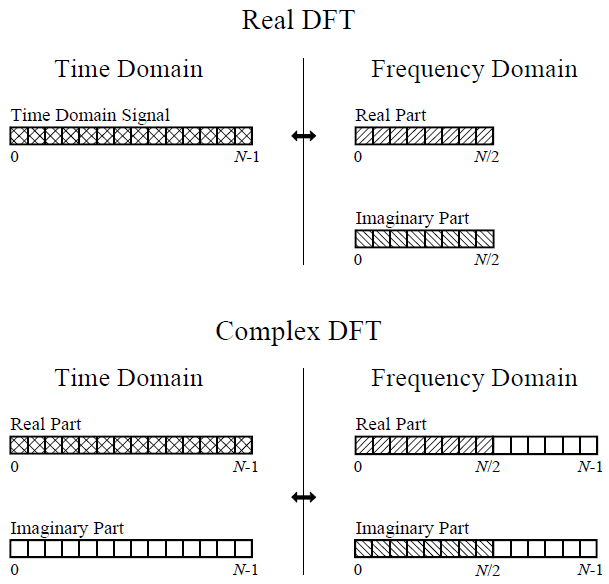
\includegraphics[width = 0.5 \textwidth ]{Graphs/ComplexDFT.png}
    \caption{Complex DFT}
    \label{ComplexDFT}
\end{figure}

En 1822, Jean Joseph Fourier montra que certaines fonctions semi-périodiques peuvent également être formulées comme une somme d'harmoniques. Une fonction semi-périodique est une fonction qui est approximent similaire d'une fonction périodique. Un example d'un fonction périodique est le $\alpha cos(x) + \beta$, etc. En théorie, un signal est représentable par une somme des sinusoïdes :
 
\begin{equation}\footnote{Curtis Roads, \textit{The Computer Music Tutorial}, 1996. [p. 1085] \nocite{Roads1996} }
    x(t) = c_0 + \sum_{n=1} ^ \infty c_n cos( \omega t + \theta_n) 
\end{equation}

Où $ t $ est la période, $ x $ est le signal, $ c_0 $ est l'harmonique fondamentale, $ k $ la fréquence, $ \omega = 2 \pi k $ et $ \theta $ est la phase de chaque harmonique . Dans cette formulation de la transformation de Fourier, il est clair qu’un son $ x $ lié au facteur de temps $ t $ peut être décrit comme une somme de sinusoïdes.

Pour cette raison, la transformation de Fourier pour toute fonction intégrable $ f: \mathbb{R} \to \mathbb{C} $ est la suivante :
 
\begin{equation}\footnote{Hermann L F. Helmholtz, \textit{The Sensations of Tone}, 1895. [p. 215] \nocite{Herm1895}}
     F[x(t)](\omega) = \int_{-\infty}^{+\infty} e ^ {-j \omega t} x(t) \hspace{1mm} dt \hspace{5mm} 
\end{equation}
    
Où $ F[x(t)] (\omega) $ ou simplement $X(\omega)$ est la transformation de Fourier du signal $ x $ bornée par sa  fréquence $ \omega $ correspondante. Dans le domaine sonore numérique, cette fréquence varie entre 0 et la fréquence d'échantillonnage (SR). Le SR est généralement 44100 ou 48000Hz. Le domaine de cette fonction pouvant être intégrée aux signaux sonores numériques varie dans l'intégrale $ [- 1, 1] $. Comme on le voit clairement dans cette formule, le facteur temporel est infini, mais un tel calcul est évidemment impossible. D'autres variations de la transformation de Fourier en temps discret sont en réalité utilisées en informatique.

         \begin{figure}
            \centering
            
\includegraphics[width = 0.5 \textwidth ]{Graphs/Fourier_Circle_1.png}
            \caption{Circle de la transformation Fourier}
            \label{CircleFourier}
        \end{figure}

La transformation de Fourier est basée principalement sur la formule d'Euler où $ e ^ {2 j \pi t} = cos (2 \pi t) + j sin (2 \pi t) $. On peut imaginer cette opération comme dessiner un cercle dans le plan complexe $ \mathbb{C} $. Au cours de la transformation de Fourier, un signal $ x(t) $ est rendu autour d'un cercle avec ($ e ^ {- j \omega t} $), avec une fréquence $ k $. Rappelons que $ \omega = 2 \pi k $. La rotation est donnée par le signe de $ j $ (nombre imaginaire). Une rotation dans le sens des aiguilles d'une montre est donc considérée comme $ -j $. Ce processus nous donne effectivement deux parties, la vraie, $ cos (2 \pi) $, et l’imaginaire, $ j \; sin (2 \pi t) $,  partie de l'équation.

On transforme souvent les données cartésiennes induites par l'exponentielle complexe en une forme polaire plus manipulable. Après la transformation de Fourier, il existe deux facteurs à manipuler, la phase et la magnitude. La phase est déduite par l'angle des deux coordonnées cartésiennes dans le plan complexe, tandis que la magnitude est déduite par le vecteur produit des deux valeurs. De la phase, on peut extraire des informations sur la fréquence du signal sur l'échantillon précise et, comme son nom l’indique, des informations de magnitude sur l’amplitude de l’échantillon exacte. Lorsque le temps est fixé pour l'exécution de l'analyse de Fourier, le signal sonore est divisé en intervalles de fréquence factorisés par la fréquence de l'analyse ($ \omega $). La phase et la magnitude sont calculées pour chaque fraction de temps sur laquelle l'analyse de Fourier est effectuée. La magnitude est égale à: $ m (x) = \sqrt{i (x) ^ 2 + r (x) ^ 2} $ et la phase est $ \theta (x) = tan ^ {- 1} (\frac{i (x)}{r (x)}) $ \ref{MagnitudePhase}. La transformation de Fourier d'un signal $x(t)$ peut etre également exprimé en termes de magnitude et phase pour chaque $k$:
$$\footnote{M.H. Serra, \textit{Musical Signal Processing}, 1996, pp. 35-37. \nocite{Roads97}} \; F[x(t)](k) = m(k) e^{j \theta(k)}.$$
ou $k$ est une fréquence typicament variée entre $(- \infty,+ \infty)$
         \begin{figure}
            \centering
            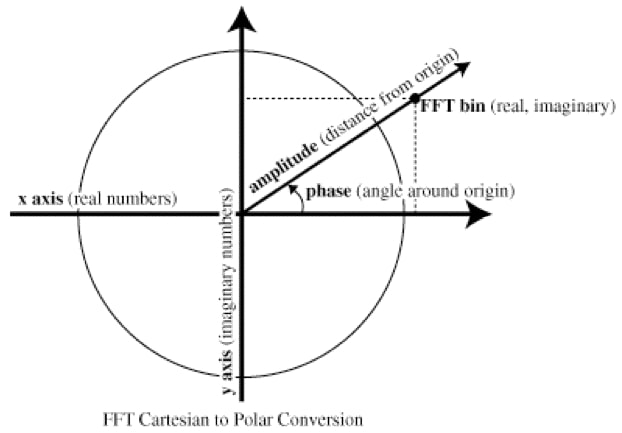
\includegraphics[width = 0.5 \textwidth ]{Graphs/Fourier_Circle_2.jpg}
            \caption{Magnitude et phase}
            \label{MagnitudePhase}
        \end{figure}

Évidemment, dans le domaine numérique, on ne peut pas utiliser une partie de temps infinie. Nous introduisons, donc, la notion de la fenêtre et, ainsi, du fenêtrage. La fenêtre est une période de temps exprimée en images. Les images sont une notion équivalente du SR en le sens que le SR calcule une quantité des trames du son par minute et que les images sont exactement ces trames. Une analyse fenêtrée est généralement exprimée par un algorithme de transformation à court terme de Fourier (STFT) \footnote{Jown Strawn, \textit{STFT : Short Time Fourier Transform}, 1985. [pp. 141– 134] \nocite{Str85} }.

\begin{equation}
\footnote{Tadej Droljc, \textit{STFT Analysis Driven Sonographic Sound Processing in Real-Time using Max/MSP and Jitter}, 2011. \nocite{Dr11} }
    X(k, \tau) = \sum_t ^ \infty x(t) (t-\tau)e ^ {-j \omega t} \hspace{5mm} 
\end{equation}

Où $x$ est le signal, $X$ sa transformation Fourier (une abréviation de la forme $F[x(t)]$), $\omega = 2 \pi k$ , $t$ le temps continue, $\tau$ l’instant temporel, $c_n$ les harmoniques, $\omega(t-\tau)$ le fenêtrage, et $j$ un nombre complexe.

Dans cette recherche, on va utiliser la forme continue TFD et puis FFT, vu que cette formule est premièrement utilisée dans Max et en plus requiert une puissance calculatrice plus efficace que d’autres méthodes :

\begin{equation}
\footnote{Jean-François Charles, \textit{ A tutorial on spectral sound processing using max and jitter}, 2008. [pp. 87–102.] \nocite{Ch08}}
    X(k) = \frac{1}{N} \sum_{n = 0} ^ {N-1} x(n+1) e ^ {-j \frac{2 \pi k n}{N}} \hspace{5mm}
\end{equation}

Où $ N $ est la taille de la fenêtre, qui correspond au nombre total d'images qu'il contient. $ X $ est le signal, $ n $ énumère chaque image dans $ N $ et $k$ varie entre $0$ et $N$. Ce formule indique que le spectre est divisé en $N$ parties. Cette division entraîne la fréquence $f_k$ qui corresponde à :

$$f_k = k \, \frac{SR}{2 N} $$

ou $SR$ est la fréquence d'échantillonnage du signal $x$. Ses points $f_k$ du spectre s’appellent bins de fréquence\footnote{M.H. Serra, \textit{Musical Signal Processing}, 1996, pp. 37-45. \nocite{Roads97}}. Le nombre des bins spectrales est toujours égal à $\frac{1}{2}$ de la taille de la DFT. Ainsi, une DFT à 1024 points produit 512 bins de fréquence. Il faut pour autant signaler la différence entre la taille de la DFT et $N$. $N$ égale toujours la moitié de la taille de une DFT. La taille de une DFT existe pour préciser la taille en échantillons du fenêtrage qui sera discuté amplement dans la section prochaine.

Pour chaque transition vers le domaine fréquentiel, une fonction inverse du domaine fréquentiel vers le domaine temporel est nécessaire. La fonction inverse se caractérise par la transformation de Fourier rapide inverse (IFFT) pour des valeurs de temps discrets.

\begin{equation}
\footnote{Alan V. Oppenheim et Ronald W. Schafer, \textit{Discrete-time signal processing}, 2009. [pp. 822 - 835] \nocite{Sch09} }
    x(n) = \frac{1}{N} \sum_{ k = 0} ^ {N-1} X(k) e ^ {j \frac{2 \pi k n}{N}} \hspace{5mm} 
\end{equation}



    \subsubsection{Transformation Fourier rapide (FFT)}

Or, la formule de Fourier générale n'est pas représentative dans le monde informatique. Pour autant, un point de vue théorique reste essentiel mais l'objectif est de se concentrer sur les formules computationnelles. Par computation, nous entendons une formule qui est facile à exécuter par un ordinateur en temps raisonnable et à produire une sortie. Une solution à cette affirmation est la transformation de Fourier rapide. Ainsi, FFT est un algorithme calculable pour DFT qui utilise un moyen intelligent pour réduire le temps de calcul et la complexité des calculs.

Nous rappelons la DFT standard interprétée dans un code informatique.

\noindent\begin{minipage}{\textwidth}
    \begin{lstlisting}[language=Python, caption= DFT]
    function DFT(x)
        N = length(x)
        # On voit deux vecteurs, un pour l'espace reel (n) et un pour l'espace de frequence (k) 
        n = 0:N-1
        k = n'
        transform_matrix = exp.(-2im*pi*n*k/N)
        return transform_matrix*x
    end.
    \end{lstlisting}
\end{minipage}

La transformation de Fourier est en réalité une matrice de calcul. Cependant, en effectuant autant de calculs, on peut imaginer que le processus est assez cher computationnellement. Les conditions requises pour la DFT sont le traitement en temps réel et des fenêtres d’une taille au puissance de 2 échantillons pour les données sonores. L'amélioration de l'algorithme a été donnée par James Cooley et John Tukey \footnote{James Cooley et John Tukey, \textit{An algorithm for the machine calculation of complex Fourier series}, 1965. \nocite{Fourier_complex}} La FFT par Cooley et Tukey est limitée aux tailles de bloc qui sont des puissances de deux.
 
L'algorithme de Cooley-Tukey utilise la récursivité pour réduire la complexité de calcul. En particulier, la matrice produite par la réduction dans le domaine fréquentiel est réduite en deux parties avant d'effectuer les calculs DFT. Nous séparons les indices impairs des casiers du même, puis la procédure est répétée. Ce processus réduit la complexité à $ \mathcal{O} (n \; log \; n) $ à partir d’une taille polynomiale. Bien sûr, pour effectuer cette action en raison de la division continue par deux, nous demandons que la fenêtre d’analyse soit une puissance de deux.

Le diagrammes au forme de “Papillon” est l'idée principale de la réduction du calcul FFT. En particulier, Cooley et Tukey ont remarqué que les exponentielles complexes sont entièrement répétées dans la seconde moitié de la fenêtre avec un signe opposé. Par conséquent, en divisant constamment la fenêtre, les calculs de l’exponentielle complexe sont considérablement réduits. Nous pouvons visualiser le processus dans la figure \ref{Butterfly} \footnote{Image récupérée de l'article: \href{https://www.researchgate.net/figure/Radix-2-butterfly-diagram-for-8- point-FFT_fig1_312460770}{P. G. Reshma, P. Gopi Varun, Babu V. Suresh, Wahid Khabou, \textit{Analog implementation of FFT using cascade current mirror}, 2017.} \nocite{FFTmirror}}.

    \begin{figure}
        \centering
        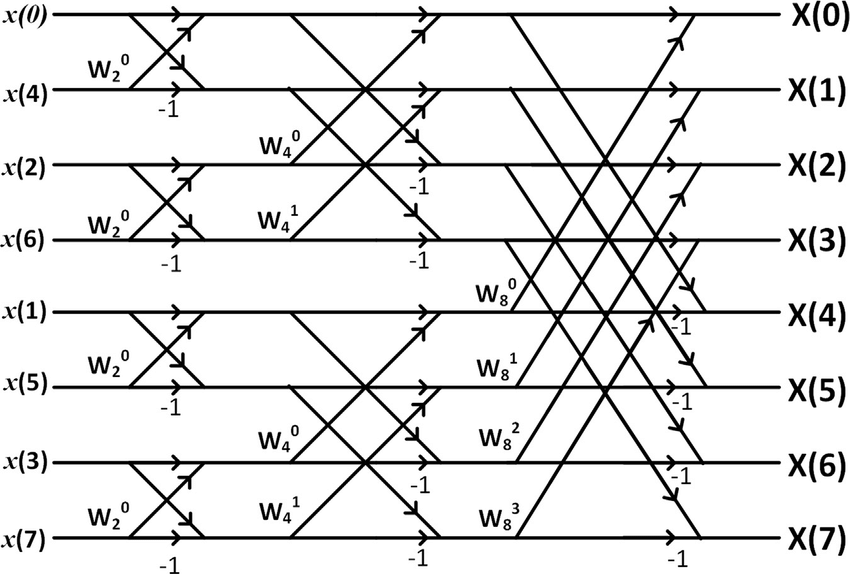
\includegraphics[width = 8cm]{Graphs/Butterfly_8-point-FFT.png}
        \caption{Diagramme papillon pour une FFT à 8 points}
        \label{Butterfly}
    \end{figure}

Une mise en œuvre du code correspondant est en disposition dans l'appendix \ref{Cooley-Tukey_Code}.

\subsection{Fenêtrage}

Pour calculer la STFT, il faut définir la taille de la fenêtre à traiter. La transformation de Fourier dans une fenêtre temporelle discrète peut produire des artefacts contredisant le continuum du signal. Pour éviter cet effet, il est habituel de multiplier la fenêtre du son d'origine par une fenêtre, qui ne contient pas des informations sonores, de la même taille sur laquelle une fonction factorise l'amplitude du son. La transformation de Fourier est reproduite un nombre dénombrable de fois en fonction de la taille du son analysé. La fenêtre est généralement beaucoup plus petite que le son d'origine, ce qui entraîne la répétition à plusieurs reprises de la fenêtre pendant la durée totale du son. Il est important que la fenêtre soit déplacée dans le temps, mais d’être également chevaucher sur lui même par un facteur de décalage. Le processus peut être décrit visuellement dans la figure \ref{overlapping}.

Cette technique, appelée chevauchement où superposition, donne un résultat sonore plus arrondi. En raison du chevauchement et de la multiplication de l'enveloppe, l'auditeur ne peut percevoir aucun des artefacts possibles induits par l'analyse mais on entend un résultat unifié \footnote {Daniel W. Griffin et Jae S. Lim, \textit{Signal estimation from modified short-time fourier transform}, 1984. \nocite{GrL84}}. De plus, le fenêtrage est une méthode pour couper un signal en plusieurs morceaux et appliquer de la transformation de Fourier au chacun de ces morceaux . Cette méthode est particulièrement efficace quand le signal n'est pas périodique. Si un signal n'a pas constamment les mêmes partiels, il est possible de regarder son développement tout au long du temps en le coupant en petites morceaux.
 
         \begin{figure}
            \centering
            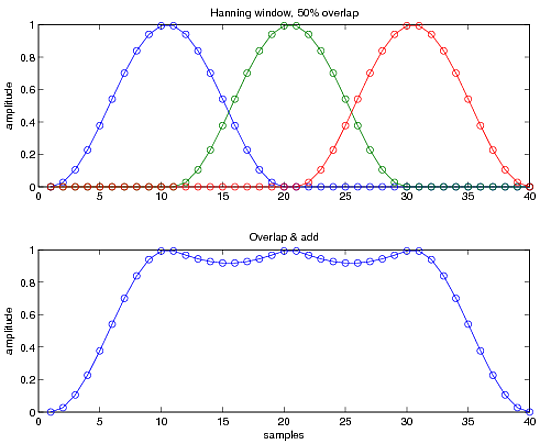
\includegraphics[width = 0.5 \textwidth ]{Graphs/Overlapping.png}
            \caption{Overlapping}
            \label{overlapping}
        \end{figure}

\subsubsection{Filtres Gabor}

Nous examinerons, ici, la possibilité d’utiliser des filtres de Gabor pour appliquer une enveloppe au signale sonore. Les filtres de Gabor sont définis comme la multiplication continue d'une fonction gaussienne par un signal complexe bornée par un facteur temporel. Le filtre gaussien est décrit dans la formule suivante \footnote{Dennis Gabor, \textit{Theory of Communication}, 1994 \nocite{Gab44}}:

\begin{equation}
    G_x(t,k) = k \int_{-\infty}^{+\infty} e ^ {-\pi(\tau-t)^2} e ^ {-j \omega \tau} x(\tau)\hspace{1mm} d\tau  
\end{equation}

Il est possible de considérer un filtre de Gabor comme deux filtres déphasés qui sont un produit direct de la décomposition de l'exponentiel complexe. L'un correspond à la partie imaginaire et l'autre à la partie réelle. Où la partie réelle a le filtre $ g_{real} (t) = \alpha w (t) sin (2 \pi \beta t + \theta) $ et la partie imaginaire $ g_{imag} (t) = w (t) cos (2 \pi f_0 t + \theta) $, oû $w(t) = e^{- \pi t}$ et $\alpha, \; \beta, \; \theta$ sont des paramètres du filtre.

Les deux filtres peuvent être déphasés mais la phase est prise en compte. Par conséquent, leur effet sur une sinusoïde est toujours une sinusoïde.

Pour manipuler la courbe d'un filtre de Gabor, il suffit de changer les paramètres. La formule normalisée se transforme en \footnote{Javier R. Movellan, \textit{A tutorial on gabor filters}, 2008. \nocite{Tut2002}}:

\begin{equation}
    G_x(t,k) = \int_{-\infty}^{+\infty} \frac{1}{\sigma \sqrt{2 \pi}} e ^ {-\frac{1}{2}(\frac{\tau-t}{\sigma})^2} e ^ {-j\omega \tau} x(\tau)\hspace{1mm} d\tau  
\end{equation}

Où $ \sigma $ est le paramètre de la courbe gaussienne. Un filtre de Gabor permettra de créer un résultat sonore plus lisse après l'analyse. La même logique est valable pour tous les types enveloppe de fenêtre tels que le hanning, le hamming, etc.

    \subsection{Le vocodeur de phase}    
    
        \subsubsection{Définition}   

Le vocodeur de phase est un outil d'analyse-synthèse qui utilise la DFT. L'analyse est effectuée de sorte que le signal de sortie théoriquement ne subisse aucune perte de données de la transformation, que ce soit théoriquement ou concrètement. Le signal de sortie est identique à l'entrée avant l'analyse si aucun traitement n'est appliqué. Les utilisations les plus courantes du vocodeur de phase sont le décalage de hauteur de ton et l’alternance de la vitesse de lecture. Le vocodeur de phase n’a pas de restriction évidente et peut également garder une trace des inharmonicités et du vibrato des sons \footnote{Johannes Grünwald, \textit{Theory, implementation and evaluation of the digital phase vocoder in the context of audio effects}, 2010. \nocite{GR10} }.       

Une manière pour décrire le vocodeur de phase consiste à représenter le signal par une séquence d'images successives d’une transformation de Fourier Discrète(TFD) d’une fenêtre de longueur $ N$. Ces images sont d'abord multipliées par une fenêtrage appropriée (telle que Hamming, Hanning, Kaiser, Blackman, etc.) puis transformés dans le domaine fréquentiel. A ce stade, toute modification prudente du spectre peut être faite, avant la transformation inverse au domaine temporel avec la transformation de Fourier discrète inverse (TDFI). Les parties d'overlap et éventuellement un fenêtrage sont additionnées, ce qui donne le résultat final.

\vspace{0.4cm}

La STFT (une transformation caractérisée des successions des TFD) d'un signal fenêtré est défini comme suit:

\begin{equation}
    X(k, \tau) = \frac{1}{N}\sum_{ n = 0 }^{ N-1 } h(n) x(n - \tau) W_N \hspace{0.05cm}^{ n k}, \hspace{1cm} \forall n \in SR 
\end{equation}

ou \hspace{0.1cm} $ W_N = e ^ {\frac{2\pi j}{N}} $ \hspace{0.1cm} et $ h(n) $ est une fenêtre approximativement choisie.

\begin{equation}
    h_k(n) = \frac{1}{N} h(n) W_N \hspace{0.05cm} ^{k \, n},\hspace{1cm}  k = 0, 1, \dots, N - 1 
\end{equation}

Pendant le processus de l'analyse, la succession des images d'une STFT font parties du signal d'entrée $x(n)$, sur la position $n_a^u = uR_a$, ou $R_a$ est nommé \textit{input hop size} et $u$ doit etre un entier. La fenêtre(ou la durée) de la DFT est définie par la taille $N$, ou le \textit{hop size} est forcément une sous-multiplication de $N$. Cet effet permettra de réaliser un \textit{overlap} de 50\%, 75\%, etc.

Le terme $\tilde{x}_u(n)$ propose l'estimation des fenêtres symétriques calculées. Donc si nous supposons un chevauchement du fenêtrage par 50 \%, ou bien $N/2$, on propose une manière d'éviter les asymétries de phase ci-dessus:  

\begin{equation}
    X[n_a^u, k] = \sum_{n=0} ^{N-1} \tilde{x}_u(n) W_N^{kn} \vspace{0.5cm} 
\end{equation}

\hspace{5cm} ou \hspace{1cm} ${x}_u(n) = h_a(n) x(n-n_a^u)$ 

Le terme $\tilde{x}_u(n)$ propose l'estimation des fenêtres symétriques calculées. Donc si nous supposons un overlap de fenêtrage par 50 \%, ou bien $N/2$, puis une manière d’éviter les assymétrages de phase est composée ci-dessus:  

\begin{equation}
    \tilde{x}(n) = x[((n-N/2))_N] 
\end{equation}

ou $((.))_N$ présente l'opération du modulo, et $N$ est la durée de la fenêtre et il devait être un pair.


Par conséquent, la transformation de Fourier du signal liée au fenêtrage devient :f

\begin{equation}
    X(k, rl) = \sum_{n=0}^{N-1} x(n) h(rl-n)  W_N^{\; k n}
\end{equation}

% C'est une fonction de deux variables discrètes, le temps $ t $ et la fréquence $ k $. L'indice $ ir $ est la position de la fenêtre, $r$ étant le numéro de l’échantillon et $l$ la taille du pas de chevauchement de la fenêtre d'analyse. $ S (rl, k) $ peut être vu comme le spectre de la multiplication $ s (m) w (rl-m) $, qui est la séquence en entrée $s (m)$ multipliée par la fenêtre décalée à la position $ rl $. Ce n'est pas le spectre exact, mais sa convolution avec la transformation de Fourier des fenêtres correspondantes.

C’est, donc, une fonction de deux variables discrètes, le temps instantané $\tau$ et la fréquence $k$. L’index $rl$ est la position de la fenêtre, $r$ étant le numéro d’image (frame) et $l$ la taille du décalage de la fenêtre d’analyse.

$ X (k, rl) $ peut être vu comme le spectre de la multiplication $ x (n) h (rl-n) $, qui est le signal d'entrée $ x (n) $ multiplié par la fenêtre décalée à la position $ rl $. Ce n'est pas le spectre exact, mais sa convolution avec la transformation de Fourier de la fenêtre.

La procédure standard de chevauchement (\textit{overlap}) consiste à additionner les buffers et à les diviser par la somme des fenêtres décalés. Le signal de sortie y(n) est exprimé comme:

\begin{equation}
    y(n) = \frac{\sum_r \bar{x}(n, rl)}{\sum_r {h}(rl - n)})
\end{equation}

Pour construire une reproduction du signal d'origine ou du signal transmuté après traitement, un iFFT est nécessaire. Dans le vocodeur de phase, cette procédure accède aux informations de phase et d'amplitude et se forme comme suit:

\begin{equation}
    \bar{y}(n, rl) = \frac{1}{N}\sum_{k=0}^{N-1} |\bar{X}(k, rl)| e^{j (\frac{2 \pi}{N} k n  + \theta(k, rl))}
\end{equation}

Ou $|X(k, rl)|$ signifie la magnitude de chaque index de fréquence $k$ et $\theta(k, rl)$ la phase de chaque index de fréquence $k$ accordinement du fenêtrage bornée par $rl$.

Enfin pour calculer la fréquence de chaque image instantanée il suffit de suivre la formule :

\begin{equation}
    \bar{f}_{k,n} = \frac{\theta(k, rl) - \theta((r - l )l, k)}{l}
\end{equation}

\subsection{Applications du vocodeur de phase} 

    \subsubsection{Time Streching}

Afin de réaliser un étirement du temps d'un son, traditionnellement, il suffit de baisser ou augmenter le rythme de sa lecture, mais cela produit également un changement de la hauteur. Le vocodeur de phase permet d'effectuer un étirement temporel sans pour autant changer la hauteur ou la qualité sonore. Afin de mieux comprendre le fonctionnement du vocodeur, il faut considérer la transformation Fourier à court terme, pour un étirement temporel. Afin de visualiser le résultat, on peut imaginer, pour chaque période de temps de la transformation Fourier appliquée, qu'une série d'harmoniques seront sauvegardées dans une fenêtre, ainsi que son facteur d'overlap. Pour changer le rythme de la lecture sans affecter la hauteur sonore, Il suffit d'éloigner ou de rapprocher les fenêtres.

Le modèle qui correspond à l'étirement temporelle est donnée par la formule suivante :

    \begin{align}
         x(n) &= \sum_{k=1}^{K(n)} A_k(n) \; e^{j \theta_k (n)} \\
         \theta_k(n) &= \theta_k(0) + \int_{0}^{n} f_k (\tau) \; d\tau
    \end{align}

Ou un signal est interprété par une somme des sinusoïdes $K(n)$ avec leur magnitude $A_k(n)$ et phase $\theta_k$ appropriées. Par la suite, la phase instantanée du $k-$ième sinusoïde, $\theta_k(n)$, est calculée par l'addition de la phase de la première échantillon $\theta_k(0)$ avec l'intégrale des fréquences $f_k (n)$. Le dernière est équivalent à $\Sigma_{n=0}^N f_k(n)$ pour une transformation discrète.

La modification temporelle est déterminée par deux paramètres parallèles, c’est à dire la modification de phase instantanée pour chaque échantillon et la modification du fenêtre du décalage (hop window). Plus précisément, le \textit{hop window} du stade de l'analyse est différent du \textit{hop window} de la synthèse.

Pour une modification temporelle par un facteur constant $\alpha$ tel que $n_k^u = \alpha n_\alpha^u$ la phase d'un étirement temporel devient \footnote{Jean Laroche et Mark Dolson, \textit{Improved Phase Vocoder}, 1999. [p. 324] \nocite{DoLa99}}:
    
    \begin{equation}
        \theta_k^u(n_k^u) = \theta_k(0) + \alpha \int_0^{n_k^u}  f_k (\tau) \; d\tau
    \end{equation}

    \subsubsection{Transposition de la hauteur}

Comme le vocodeur de phase peut être utilisé pour réaliser un étirement temporel d'un son sans affecter sa hauteur, il devrait également être possible de faire l'inverse, c’est-à-dire changer la hauteur sans changer le rythme de la lecture. En effet, cette opération est facilement accomplie. La procédure est de changer le rythme de la lecture par le facteur de changement de la hauteur souhaitée, puis de jouer le résultat sonore produit à une fréquence d'échantillonnage \guillemotleft incorrecte \guillemotright. Par exemple, pour augmenter la hauteur d’une octave, le son est d'abord agrandi d'un facteur de deux, et il est ensuite joué à deux fois l'original taux d'échantillonnage. \footnote{Mark Dolson, \textit{ The phase vocoder}, 1986. \nocite{Dol86}}

    \subsubsection{Freeze}

À cet effet, nous prenons une certaine fenêtre d’analyse à partir du son sélectionné et nous «gèlons» ce son dans le temps. Pour achever cet effet il s'agit de rendre le rythme de la lecture de notre vocodeur de phase à zéro. Cela peut se comparer à un étirement sonore infini. On peut ainsi appliquer les mêmes principes d'un étirement sonore normal.

    \subsubsection{Robotisation}

Pour faire une robotisation d'un signal, il faut mettre la phase de chaque échantillon à zéro. Cet effet résulte d'un son robotisé et métallique.

    \subsubsection{Harmonisation - chuchotement}

Pour réaliser cet effet on doit donner une valeur aléatoire soit à la phase, soit à la magnitude de chaque échantillon de la fenêtre de la FFT \footnote{Johannes Grünwald, \textit{ Theory, implementation and evaluation of the digital phase vocoder in the context of audio effects}, 2010. \nocite{GR10}}.

    \subsubsection{Morphing}
    
La définition générale du morphing consiste à combiner deux (ou plusieurs) éléments distincts en une seule entité qui contient les deux éléments. Le processus de morphing dépend généralement d’une seule variable, qui est appelée, un facteur de morphing ou une interpolation. Ce processus dépend, par ailleurs, du facteur temporel puisque le morphing est un phénomène dynamique.

\begin{equation}\footnote{Axel Roebel, \textit{Morphing sound attractors}, 1999. \nocite{Rob99}}
    \begin{split}
        M(\alpha, t) = \alpha(t)\widehat {S_1} + [1 -\alpha(t)]\widehat {S_2}  \\ 
        & \textrm{Ou } \alpha(t) \in [0:1]
    \end{split}
\end{equation}

La manipulation du paramètre $\alpha$ nous permettra de changer la dynamique du morphing. Traditionnellement, la fonction de manipulation agit d'une fonction linéaire. En extension, on peut s’attendre d’un autre type de fonction de manipulation que d’une fonction linéaire. Nous proposons alors d’effectuer une manipulation de $\alpha$ sur une courbe exponentielle ou logarithmique(ex. sur la figure \ref{alpha_interp}).

    \begin{figure}
        \caption{Interpolation du facteur $\alpha $}
        \label{alpha_interp}
        \begin{tikzpicture}
        \begin{axis}[
            axis lines = left,
            xlabel = $x$,
            ylabel = {$f(x)$},
        ]
        
        \addplot [
            domain= 0:1, 
            samples=100, 
            color=blue,
        ]
        {log10(9*x+1)};
        \addlegendentry{$log(9x+1)$}
        \end{axis}
        \end{tikzpicture}
        \begin{tikzpicture}
        \begin{axis}[
            axis lines = left,
            xlabel = $x$,
            ylabel = {$f(x)$},
        ]
        
        \addplot [
            domain= 0:1, 
            samples=100, 
            color=blue,
        ]
        {exp(5*(x-1))};
        \addlegendentry{$e^{5(x-1)}$}
        \end{axis}
        \end{tikzpicture}
    \end{figure}
        

La différence fondamentale entre le morphing d’une image, est le rapport à la variable temporelle. Le son est un phénomène dynamique, donc il ne peut pas être interpolé linéairement. Le terrain du morphing sonore nécessite des fonctions multiples pour atteindre un résultat satisfaisant. Pour obtenir un morphing sonore, il faut calculer l’enveloppe spectrale de notre FFT.

\subsubsection{Noise modeling}

Le vocodeur de phase tel qu'il est présenté jusqu'à présent est un modèle fin mais il ne s'agit toutefois pas du modèle complet. Le modèle présenté ici est celui de Xavier Serra \footnote{Curtis Roads et autres, \textit{Traitement du signal musical}, 1997. [p. 91 - 122] \nocite{Roads97}}. Dans ce modèle, les composantes sonores sont idéalisées comme déterministes. Cela suggère que chaque composant sonore est une sinusoïde ou une sinusoïde à variation lente. La partie non déterministe implique que le son est modélisé avec une composante de bruit supplémentaire, comme le montre la formule ci-dessous.

\begin{equation}\footnote{Curtis Roads, \textit{Musical Signal Processing}, 1997, p. 94}
    s(t) = \sum_{n=0}^N A_n(t) cos(\theta_n(t)) + \epsilon(t) 
\end{equation}

Où $ A_n $ et $ \theta_n $ sont respectivement l'amplitude et la phase de la n-ième fréquence. En supposant que $ \epsilon (t) $ soit un composant stochastique, il peut être considéré comme un bruit blanc filtré.

\begin{equation}
    \epsilon(t) = \int_0^t h(t, \tau) u(\tau) \; d\tau 
\end{equation} 

Où $ u (\tau) $ est un bruit blanc et $ h (t, \tau) $ nous la réponse d'un filtre variant dans le temps qui affiche une valeur au temps $ t $.

    \subsubsection{Stochastic Modeling}

Une autre méthode suggère une approche stochastique simultanée au vocodeur de phase traditionnel. Afin de appliquer une prédiction sur un signal, il est nécessaire de établir une hypothèse. L'hypothèse pour la construction stochastique du vocodeur de phase est fait sur la périodicité de signaux. Les signaux dans cette approche ont toujours une nature semi-périodique. On peut calculer d'après l'hypothèse un facteur d'erreur entre le résultat obtenu et le résultat prédit:

\begin{equation*}
    Err_{p \to q} = \sum_{n=1}^N E_\omega(\Delta f_n, f_n a_n, A_{max})
\end{equation*}

Où $ \Delta f_n $ est la différence entre un pic mesuré et le plus proche mesuré. $ f_n $ est la fréquence du $n-$ième bin et $ a_n $ est la magnitude des pics prédits. $ A_ {max} $ est la magnitude maximale enregistrée.

\begin{equation*}
    Err_{q \to p} = \sum_{k=1}^K E_\omega(\Delta f_k, f_k a_k, A_{max})
\end{equation*}

Maintenant, $ \Delta f_k $ est la différence entre un pic mesuré et son pic prédit le plus proche. $ f_n $ est la fréquence de la corbeille et $ a_n $ est la magnitude des pics enregistrés.

L'erreur totale est:

\begin{equation}\footnote{Curtis Roads, \textit{Musical Signal Processing}, 1997, p. 103 \nocite{Roads97}}
    Err_{total} = Err_{p \to q}/N + Err_{q \to p}/K
\end{equation}
\chapter{Design}

\label{ch:Design}

Dans ce chapitre, nous allons implémenter, dans le langage du logiciel Max, les formules mathématiques présentées précédemment. De plus, nous allons introduire d'autres effets spectraux et des variations dans le contexte du vocodeur de phase.

Par ailleurs, nous allons presenter les objets Max qui encapsulent\footnote{Encapsuler : créer un sub-patch qui contient un ensemble d'objets / fonctions } des fonctions mathématiques telles que FFT, IFFT et d’autres transformations. On peut attendre de ce partie qu'il permet de comprendre la plupart des outils spectraux que Max offre à l’utilisateur. Parallèlement, on va construire une série d’outils efficaces pour structurer un simple vocodeur de phase.

\section{Objets Max}

Dans cette section, nous allons mentionner quelques-uns des objets spectraux de base de Max fournis directement par la librairie standard, et nous analyserons leurs fonctionnalités.

Dans Max, il existe 3 catégories d’objets :
\begin{enumerate}
    \item
    Les objets logiques utilisés pour les expressions et les calculs logiques; 
    \item
    Les objets signaux, pour le traitement du signal, suivis généralement par une indication \guillemotleft$ \thicksim $\guillemotright après leur nom ; 
    \item
    Les objets Jitter qui sont utilisés pour les données multidimensionnelles, tels que images, formes 3D, etc.
\end{enumerate}

La manière dont un objet spectral fonctionne dans Max est quelque peu différente de celle des autres objets signaux. Ils sont déployés dans un environnement spécial appelé \textit{PFFT}$\thicksim $. Le PFFT contient, fréquemment, une FFT et une IFFT. La majorité des objets dans le PFFT traitent des données bidimensionnelles, par conséquent, ils sont traités dans un patch différent.

\subsubsection{FFT$\thicksim$}
    L'objet $ \textit{fft}\thicksim $ appartient à la famille de signaux, comme le précise l'indicateur $ \thicksim $. C'est l'objet qui effectue la transformation rapide de Fourier. Il y a deux entrées correspondantes aux parties réelle et imaginaire. Ordinairement, on utilise l'entrée réelle afin de effectuer une FFT a un signal. Il y a trois sorties a l'objet, une pour la partie réelle de l'exponentielle complexe, une pour la partie imaginaire et un compteur qui garde l’index des harmoniques de la transformation de Fourier.

    Dans la transformation de Fourier fenêtrée habituelle:
    \begin{equation}
        X_k = \sum_{n=0}^{N-1} x_n \; e^{-j \frac{2 \pi k n}{N}}
    \end{equation}

    Où k est l’indice de l'harmonique et les coordonnées complexes correspondantes sont $ \sum_{n = 0}^k x_n + cos (2 \pi t) $ pour la partie réelle et $ \sum_{n = 0}^k x_n + j sin (2 \pi t) $ pour l’imaginaire. Bien entendu, la réduction correspondante de la ramification calculée est appliquée par l’algorithme FFT présenté au chapitre précédent.

\subsubsection{IFFT$\thicksim$}
    
    De manière similaire, la FFT inverse est traitée par la fonction d'objet appropriée avec les entrées et les sorties inverses.

\subsubsection{cartopol$\thicksim$}
    
    Il n’est généralement pas utile d’utiliser ces coordonnées cartésiennes, produites par le \textit{fft}$\thicksim $ correspondant aux parties réels et imaginaires du plan $ \mathbb {C}^2 $. Par conséquent, un objet transformant les coordonnées cartésiennes en une forme polaire appelée \textit{cartopol}$\thicksim $ est fréquemment déployé. Cet objet a donc deux entrées (réelle et imaginaire) et génère une phase et une magnitude pour chaque index.

\subsubsection{poltocar$\thicksim$}
    
    Exactement la fonction inverse de \textit{cartopol}$\thicksim $. L’objet \textit{poltocar}$\thicksim $ transforme des coordonnées polaires (deux entrées) aux coordonnées Cartésiennes (deux sorties).

\subsubsection{FFTinfo$\thicksim$}
    
    \textit{FFTinfo}$\thicksim $ est très fréquemment utilisé et il fournit des informations sur les paramètres de la FFT, tels que la taille de la fenêtre, etc.

\subsubsection{\textit{framedelta}$\thicksim$}
    
    \textit{framedelta}$\thicksim$ est un objet très important car il calcule la dérivation de phase entre des images successives de la FFT. Également l'objet \textit{phaseaccum}$\thicksim$ peut etre utilisé à la place de \textit{framedelta}$\thicksim$. \textit{phaseaccum}$\thicksim$ qui calcule directement la phase après la derivation.

\subsubsection{gen$\thicksim$}
    
    \textit{gen}$\thicksim$ est un objet qui permet de créer une nouvelle fenêtre speciale d’un patch. Dans cette fenêtre, l'utilisateur peut utiliser un nouvel ensemble de fonctions spécialisées sur le traitement d'un seul échantillon. Les fonctions sont relativement plus simples que l'environnement de codage habituel, mais on peut effectuer un travail plus précis sur les détails. L’environment \textit{gen}$ \thicksim $ est fréquemment utilisé pour effectuer un délai à l'échelle d'échantillons en créant un filtre passe-bas ou des effets similaires.

\section{Détection du pitch}\footnote{Pitch signifie un terme équivalent à la hauteur ou bien à la fréquence}

En utilisant certains de ces objets spectraux Max, nous allons commencer par construire un simple patch afin de trouver la hauteur de la fréquence dominante:

     \begin{displayquote}
         \guillemotleft Les méthodes de détection du pitch dans le domaine fréquentiel dissèquent le signal d'entrée en fréquences constituant le spectre global. Le spectre montre la force des différentes composantes des fréquences contenues dans le signal. Le but est d’isoler la fréquence dominante, ou "pitch", hors du spectre \guillemotright. \footnote{Curtis Roads, \textit{A tutorial in musical signal processing}, 1996. [p. 513], \nocite{Roads1996}}
     \end{displayquote}

De même, nous avons implémenté un patch Max pour trouver la fréquence dominante de la fenêtre FFT. Le patch peut être trouvé dans la figure \ref{PitchTracking}.

    \begin{figure}
        \centering
        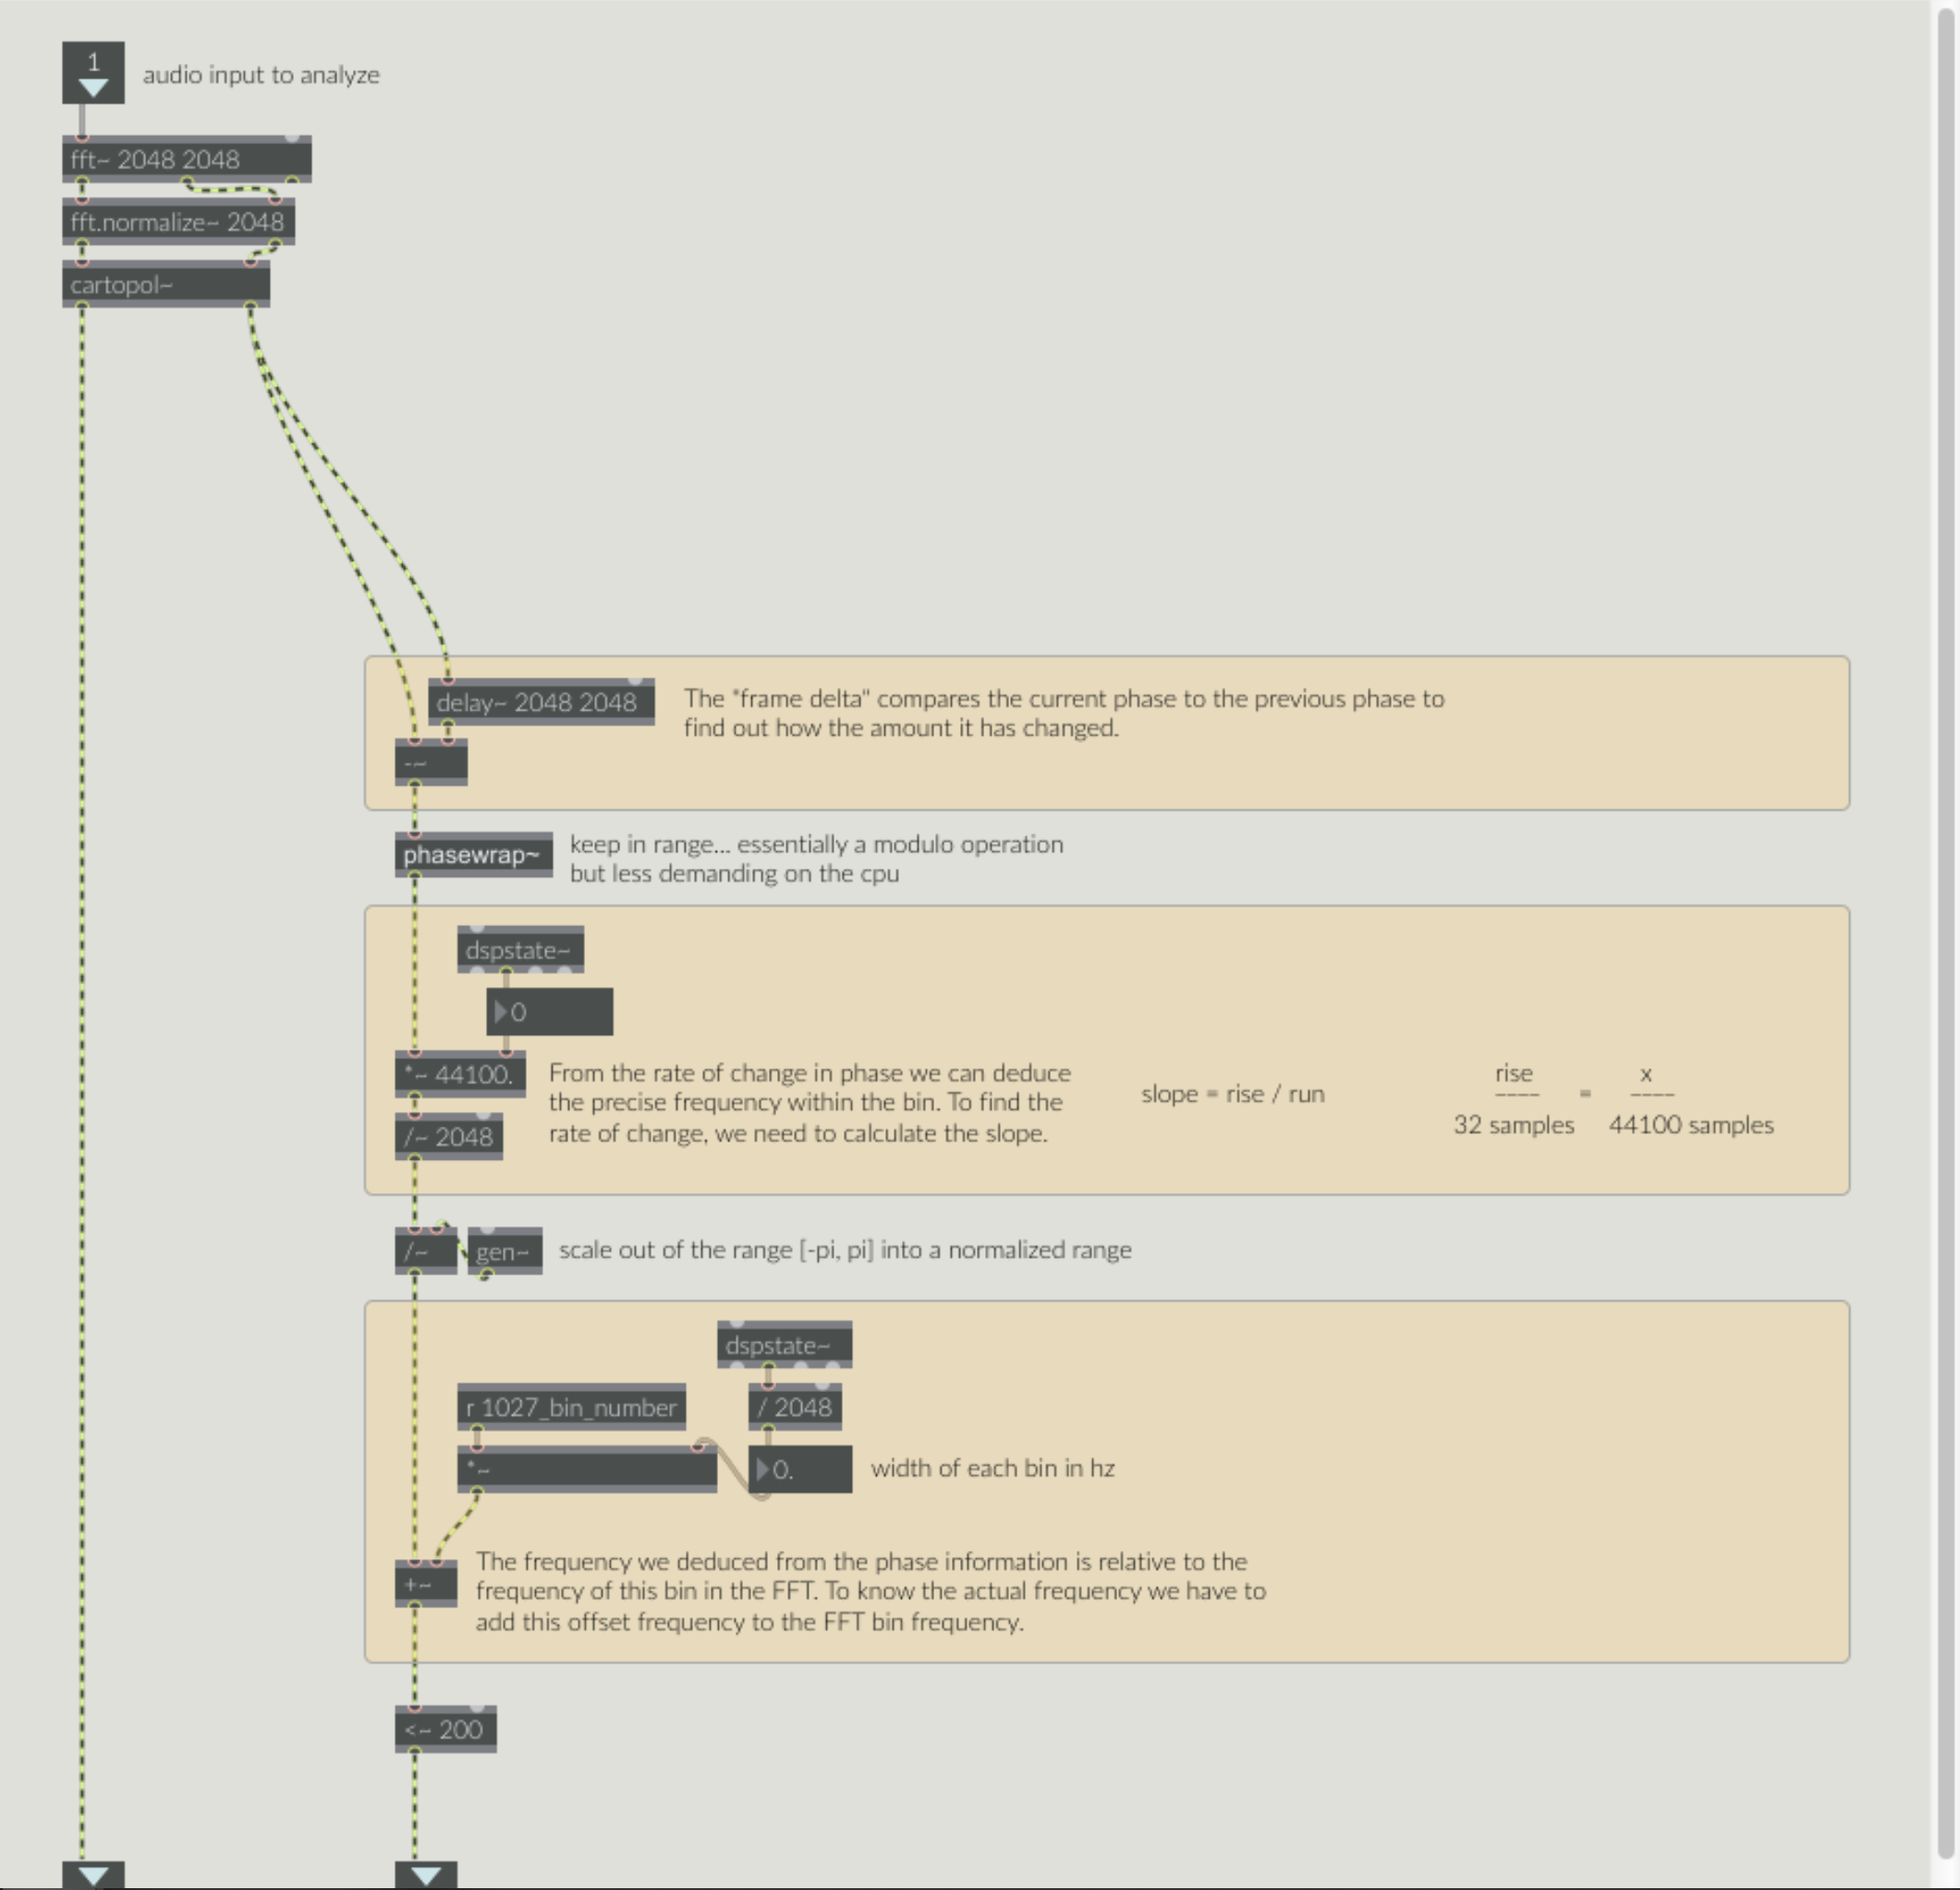
\includegraphics[width = 0.7 \textwidth ]{Graphs/fftTrack.png}
        \caption{Pitch Tracking}
        \label{PitchTracking}
    \end{figure}

Bien entendu, nous utilisons l'objet  \textit{fftin}$\thicksim $ pour transformer le son d’entré dans le domaine fréquentiel. Dans la FFT, nous devons déclarer deux choses. Tout d'abord, le nombre d'images faisant l'objet d'une opposition à la FFT et, deuxièmement, la taille de la fenêtre. Nous rappelons que les deux premières sorties donnent respectivement les composantes réelles et imaginaires. La troisième sortie donne l'harmonique de la fréquence indexée prenant les valeurs correspondantes de $ 0 $ à $ N $, où $ N $ est la taille de la fenêtre FFT.

Pour continuer le patch du simple suivi de la hauteur, nous normalisons les composants réels et imaginaires pour restreindre le flux de données entre des limites calculables. De manière plus détaillée, \textit{fft.normalize}$\thicksim $ est un simple Max externe, créé en code $C++$ à l'aide du Max SDK, qui divise le nombre de chaque sortie par la moitié de la taille de la fenêtre.

Ensuite, nous transformons les coordonnées cartésiennes en coordonnées polaires en utilisant \textit{cartopol}$\thicksim $. Le processus est expliqué à la section 2 sous les termes phase et magnitude. Nous ne sommes intéressés que par la phase de chaque bin. En utilisant la phase de chaque bin, nous pouvons calculer la fréquence exacte de chaque harmonique. Nous rappelons que les termes harmonique, bin et fréquence de Fourier sont les mêmes dans ce contexte.

Tout d'abord, nous retardons la phase de chaque bin d'une fenêtre entière pour calculer le montant de sa dérivation. Ensuite, nous soustrayons la phase en cours de chaque bin par la phase correspondante de la fenêtre précédente. Dans la suite, nous utilisons l’objet \textit{phasewrap}$ \thicksim $ pour découper la valeur comprise entre $ - \pi $ et $ \pi $. Il s'agit essentiellement d'une fonction modulo qui permet de conserver les valeurs dans un intégral computable.

À ce stade, nous devons consulter nos paramètres sonores. Un objet dans Max appelé \textit{dspstate}$ \thicksim $ récupère toutes les données nécessaires que nous pouvons trouver dans $ / Options / Audio \, Status $ dans l'application Max. Nous avons seulement besoin de la fréquence d'échantillonnage. Cette valeur est généralement $ 44100 $Hz donc on la stocké par avance et si elle différente nous la changerions automatiquement. Le signal obtenu à partir de \textit{phasewrap}$ \thicksim $ est multiplié par la fréquence d'échantillonnage et par la suite divisé par la taille de la fenêtre. Ces opérations, qui divisent le SR par la taille de la fenêtre, déduisent des partitions pondérées du spectre. La valeur de la soustraction de la fréquence classe la déviation des partitions fréquentielles. Plus précisément, on divise le spectre audible dans des parties isométriques qui sont déterminées par la division du SR par la taille de la fenêtre. Ensuite, nous normalisons en multipliant par $ 2 \pi $ stocké dans un objet \textit{gen}$\thicksim $, pour manipuler la précision sur le nombre $\pi$. Nous trouvons la position de la partition en multipliant la valeur de la division du spectre par l'indice de l’harmonique correspondante et en l'ajoutant à la déviation pour obtenir la fréquence de cette harmonique.

La division du spectre ou la partition est donnée par:
    \begin{equation*}
        x = \frac{SR}{\text{window size}}
    \end{equation*}

Ensuite, la fréquence est simplement: $ index * x + $ la déviation de phase.

Cette procédure génère toutes les fréquences de toutes les bins de la fenêtre FFT.

L'étape suivante consiste à conserver la fréquence avec la magnitude la plus forte. Nous allons utiliser un objet $ gen \thicksim $. Nous déclarons d'abord les entrées. Nous n'avons besoin que de trois variables. La magnitude de chaque bin, l’index de chaque bin et la taille de la fenêtre FFT. Nous déclarons une seule sortie pour le bin dominant de chaque fenêtre. Le patch est montré dans la figure ci-dessous.
        
    \begin{wrapfigure}{r}{0.5\textwidth}
      \vspace{-20pt}
      \begin{center}
        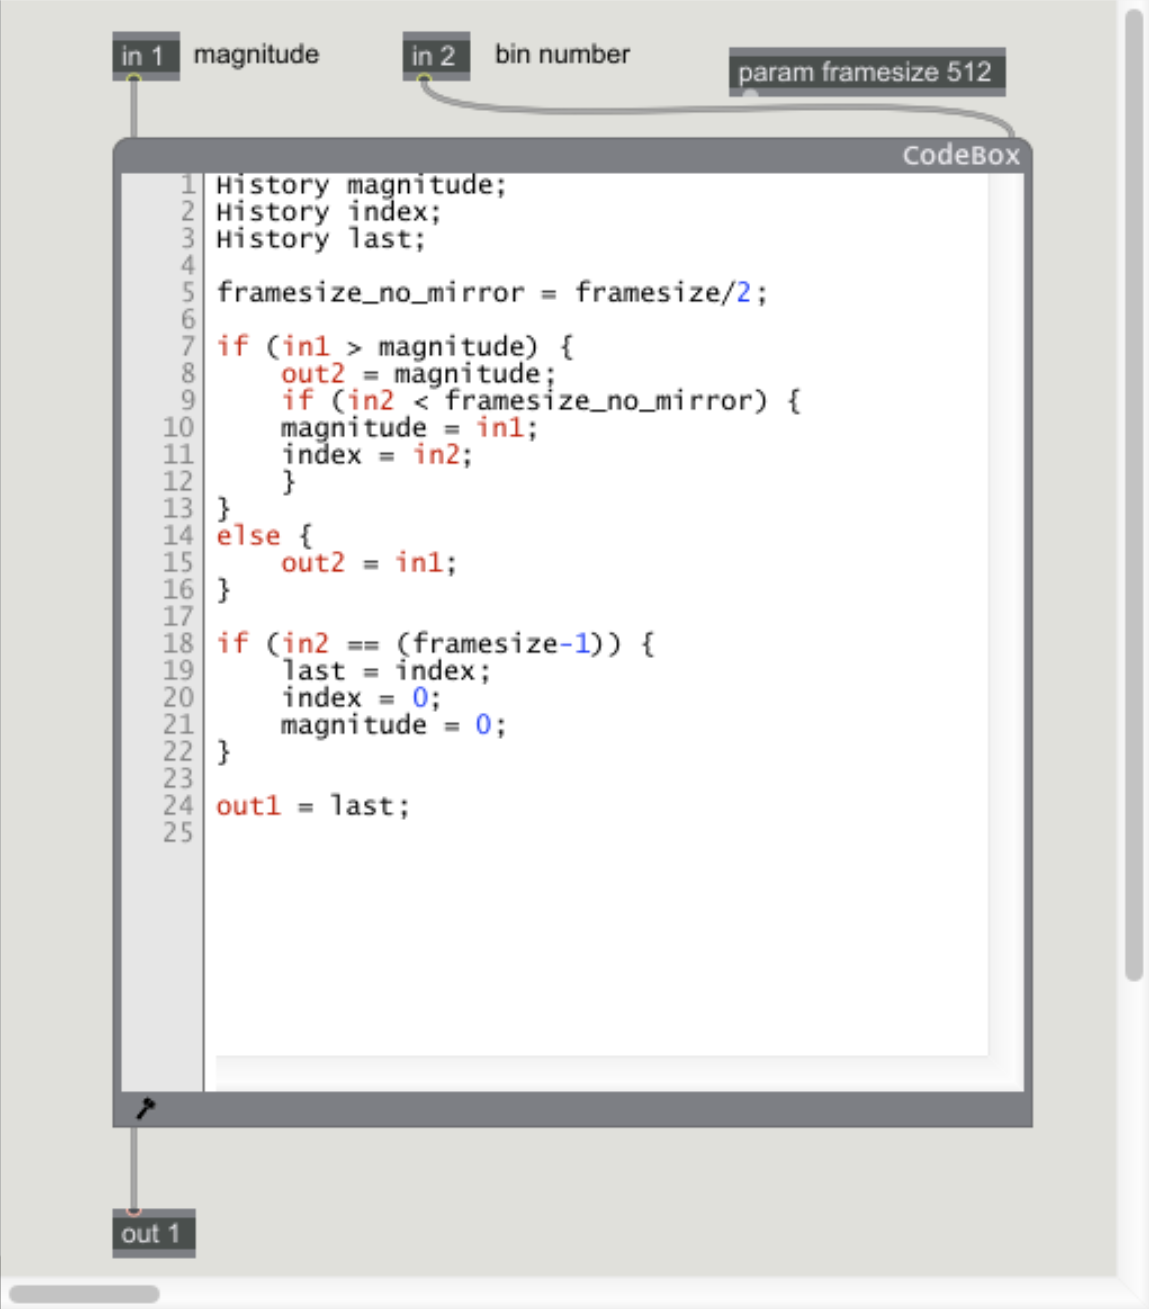
\includegraphics[width=0.48\textwidth]{Graphs/GenfftTrack.png}
      \end{center}
      \vspace{-20pt}
      \caption{Codebox$\thicksim$}
      \vspace{-10pt}
    \end{wrapfigure}

    % \begin{figure}
    %     \centering
    %     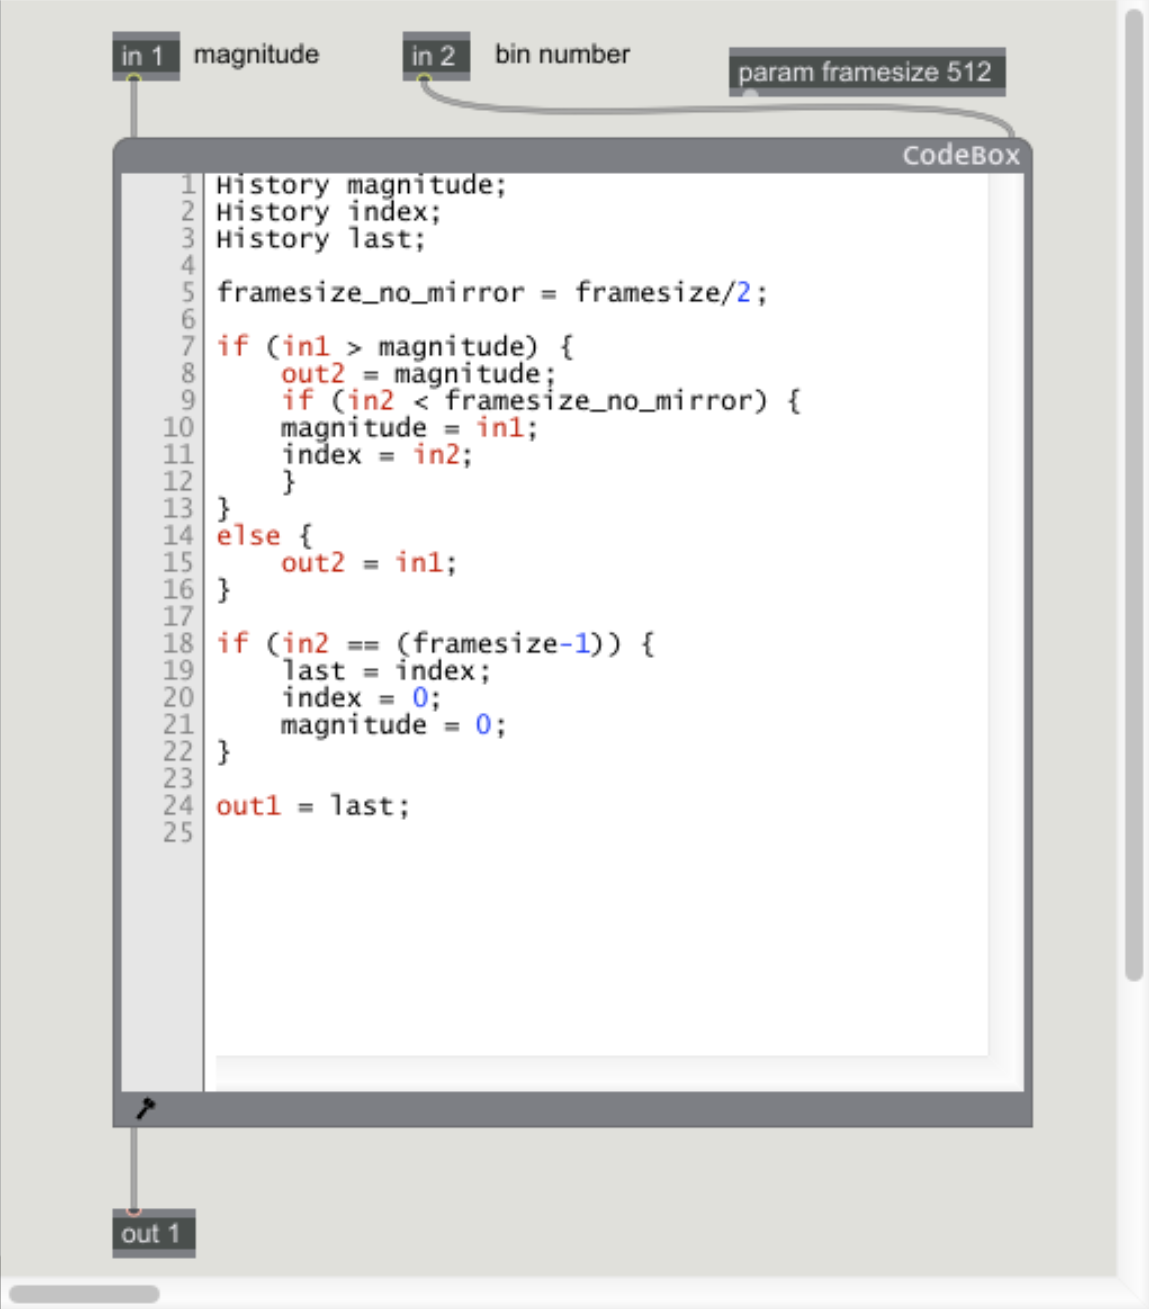
\includegraphics[width = 0.4 \textwidth ]{Graphs/GenfftTrack.png}
    %     \caption{Codebox$\thicksim$}
    %     \label{GenSingle}
    % \end{figure}

Pour calculer le bin le plus fort, nous allons utiliser un objet appelé $ codebox $. $ Codebox $ est un objet qui permet à l'utilisateur de saisir un code sous la forme \guillemotleft traditionnelle \guillemotright. Tout comme le code javascript, nous devons déclarer les variables que nous allons utiliser, qui sont suivant aussi les entrées de cet objet. Les variables dans ce cas sont: magnitude, index, frameSize et last. Où frameSize est la taille de la fenêtre FFT et last est juste une variable qui stocke l'index du bin le plus fort pour la fenêtre précédente.

Le processus de définition du bin le plus fort est mis en œuvre par deux fonctions $if$ imbriquées. Ce processus sera répété pour chaque fenêtre et il déterminera éventuellement les fréquences des cellules les plus puissantes dans toutes les fenêtres. Dans la boucle $if$ imbriquée, nous déterminons si l'index actuel est plus fort que le précédent et nous retournons le résultat. Cela signifie que si la magnitude du $ n-$ième bin est supérieure à celle du ($n-1)-$ième bin, nous stockons sa valeur d'index. La dernière étape consiste à limiter le nombre d'index dans la limite de la taille de la fenêtre afin de terminer la boucle et de réinitialiser les variables.


    \begin{figure}
        \centering
        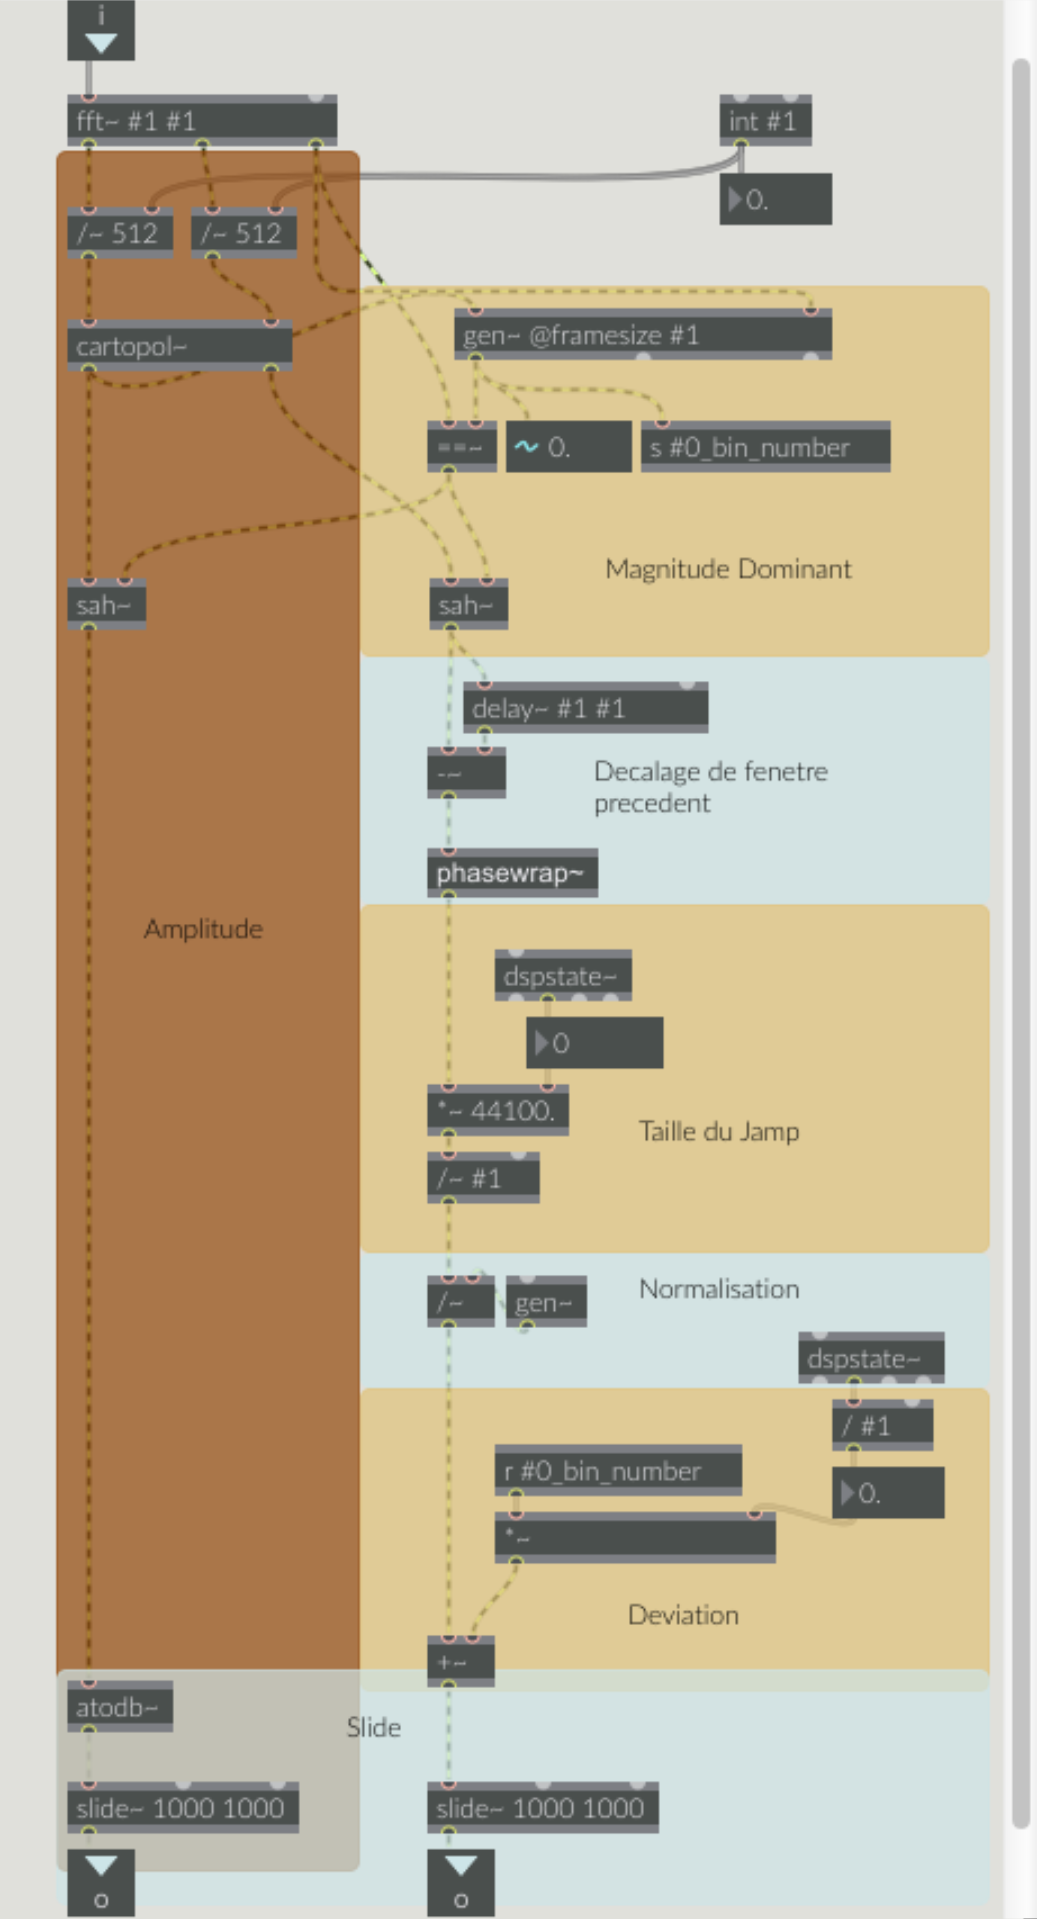
\includegraphics[width = 0.8 \textwidth ]{Graphs/ffttracker.png}
        \caption{Pitch Tracker}
        \label{PitchTracker}
    \end{figure}

Pour localiser l’harmonique le plus fort en précisant la fréquence, quelques fonctions supplémentaires sont nécessaires. La sortie de l'objet \textit{gen}$\thicksim $ est filtrée par un objet \textit{sah}$ \thicksim $. \textit{Sah}$\thicksim $ signifie  \guillemotleft sample holder \guillemotright (stockage d'un échantillon). Avant cela, l'index actuel est comparé à la valeur d'index générée par l'objet \textit{gen}$\thicksim $.  Cette fonction filtre la première entrée de l'objet par un facteur similaire à l'objet \textit{gate}$\thicksim $. Chaque fois que la valeur du facteur change, elle permet à la première entrée d'aller de l'avant et de sortir sa valeur. Nous l'utilisons deux fois, une fois pour la magnitude et une fois pour la phase. De cette façon, seul l’indice de l'harmonique avec la plus grande magnitude va de paire avec la magnitude et la phase correspondante. Nous utilisons le système fourni précédemment pour trouver la fréquence exacte et nous traduisons les coordonnées polaires de l'amplitude en dB. Enfin, nous utilisons un objet \textit{slide}$\thicksim $ pour lisser le résultat. Le patch final est montré dans la figure \ref{PitchTracker}. Cette méthode évite de calculer chaque fois la fréquence si le son est périodique et donc la fréquence dominante ne change pas.

\subsection{Détection des pitchs multiples}

Pour créer un patch de suivi des hauteurs multiples, nous utilisons la méthode du suivi de la hauteur simple unique avec quelques modifications. La majorité des calculs ont lieu dans l'objet $ gen \thicksim $ car l'implémentation de $ codebox $ est copiée en fonction du nombre de hauteurs que l'on souhaite calculer.

    \begin{figure}
        \centering
        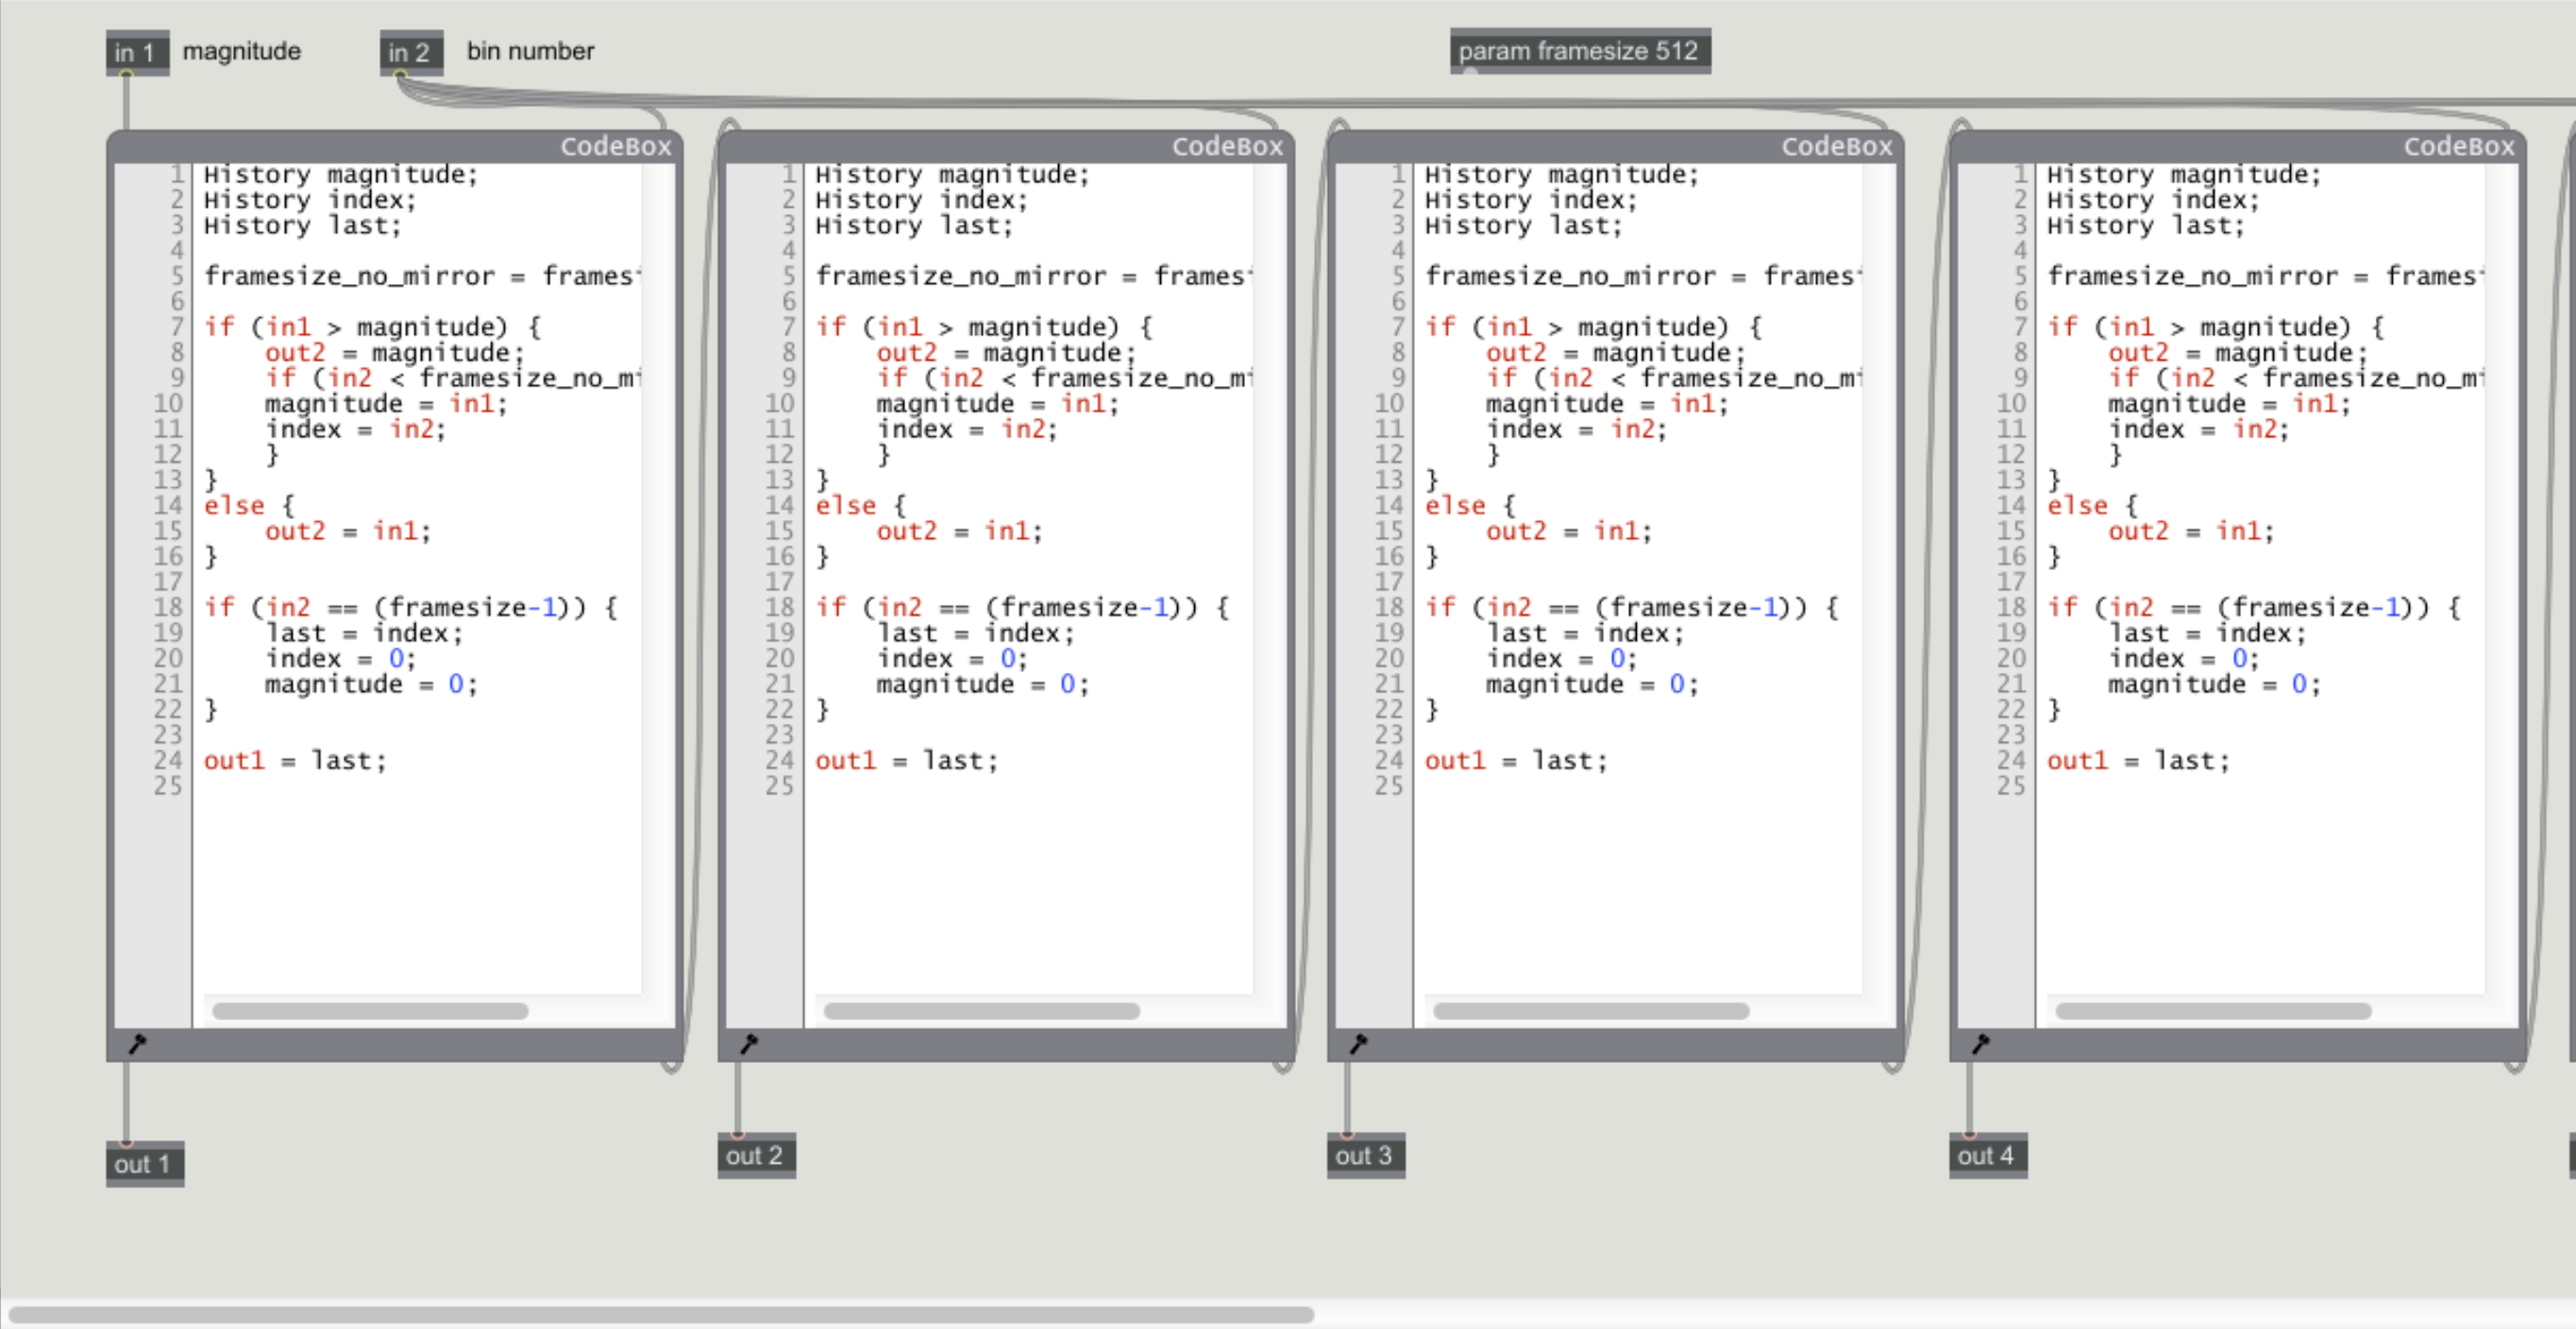
\includegraphics[width = \textwidth]{Graphs/GenMultiple.png}
        \caption{Gen multiple}
        \label{GenMultiple}
    \end{figure}

La figure \ref{GenMultiple} permet de visualiser comment on peut calculer une série des harmoniques les plus fortes de chaque fenêtre. L'objectif est de fournir une quantité suffisante d'informations sur les composantes spectrales de base du son.

Comme le suggère la figure \ref{GenMultiple}, la sortie de chaque \textit{codebox} correspond à l'entrée de la suivante, calculant ainsi le prochain indice le plus fort de la fenêtre. La quantité d’objets \textit{codebox} utilisée correspond au nombre des harmoniques que nous allons afficher.

La mise en œuvre de la méthode de la localisation des plusieurs hauteurs peut être montrée à la figure \ref{Analysis}. Nous reproduisons essentiellement le calcul de fréquence pour chaque indice. Le résultat peut être affiché sous forme de liste ou dans différents sorties. Ensuite, on peut utiliser l’objet \textit{mc.cycle$\thicksim $} dans la version Max8, de simples oscillateurs ou résonateurs dans les autres cas.

    \begin{figure}
        \centering
        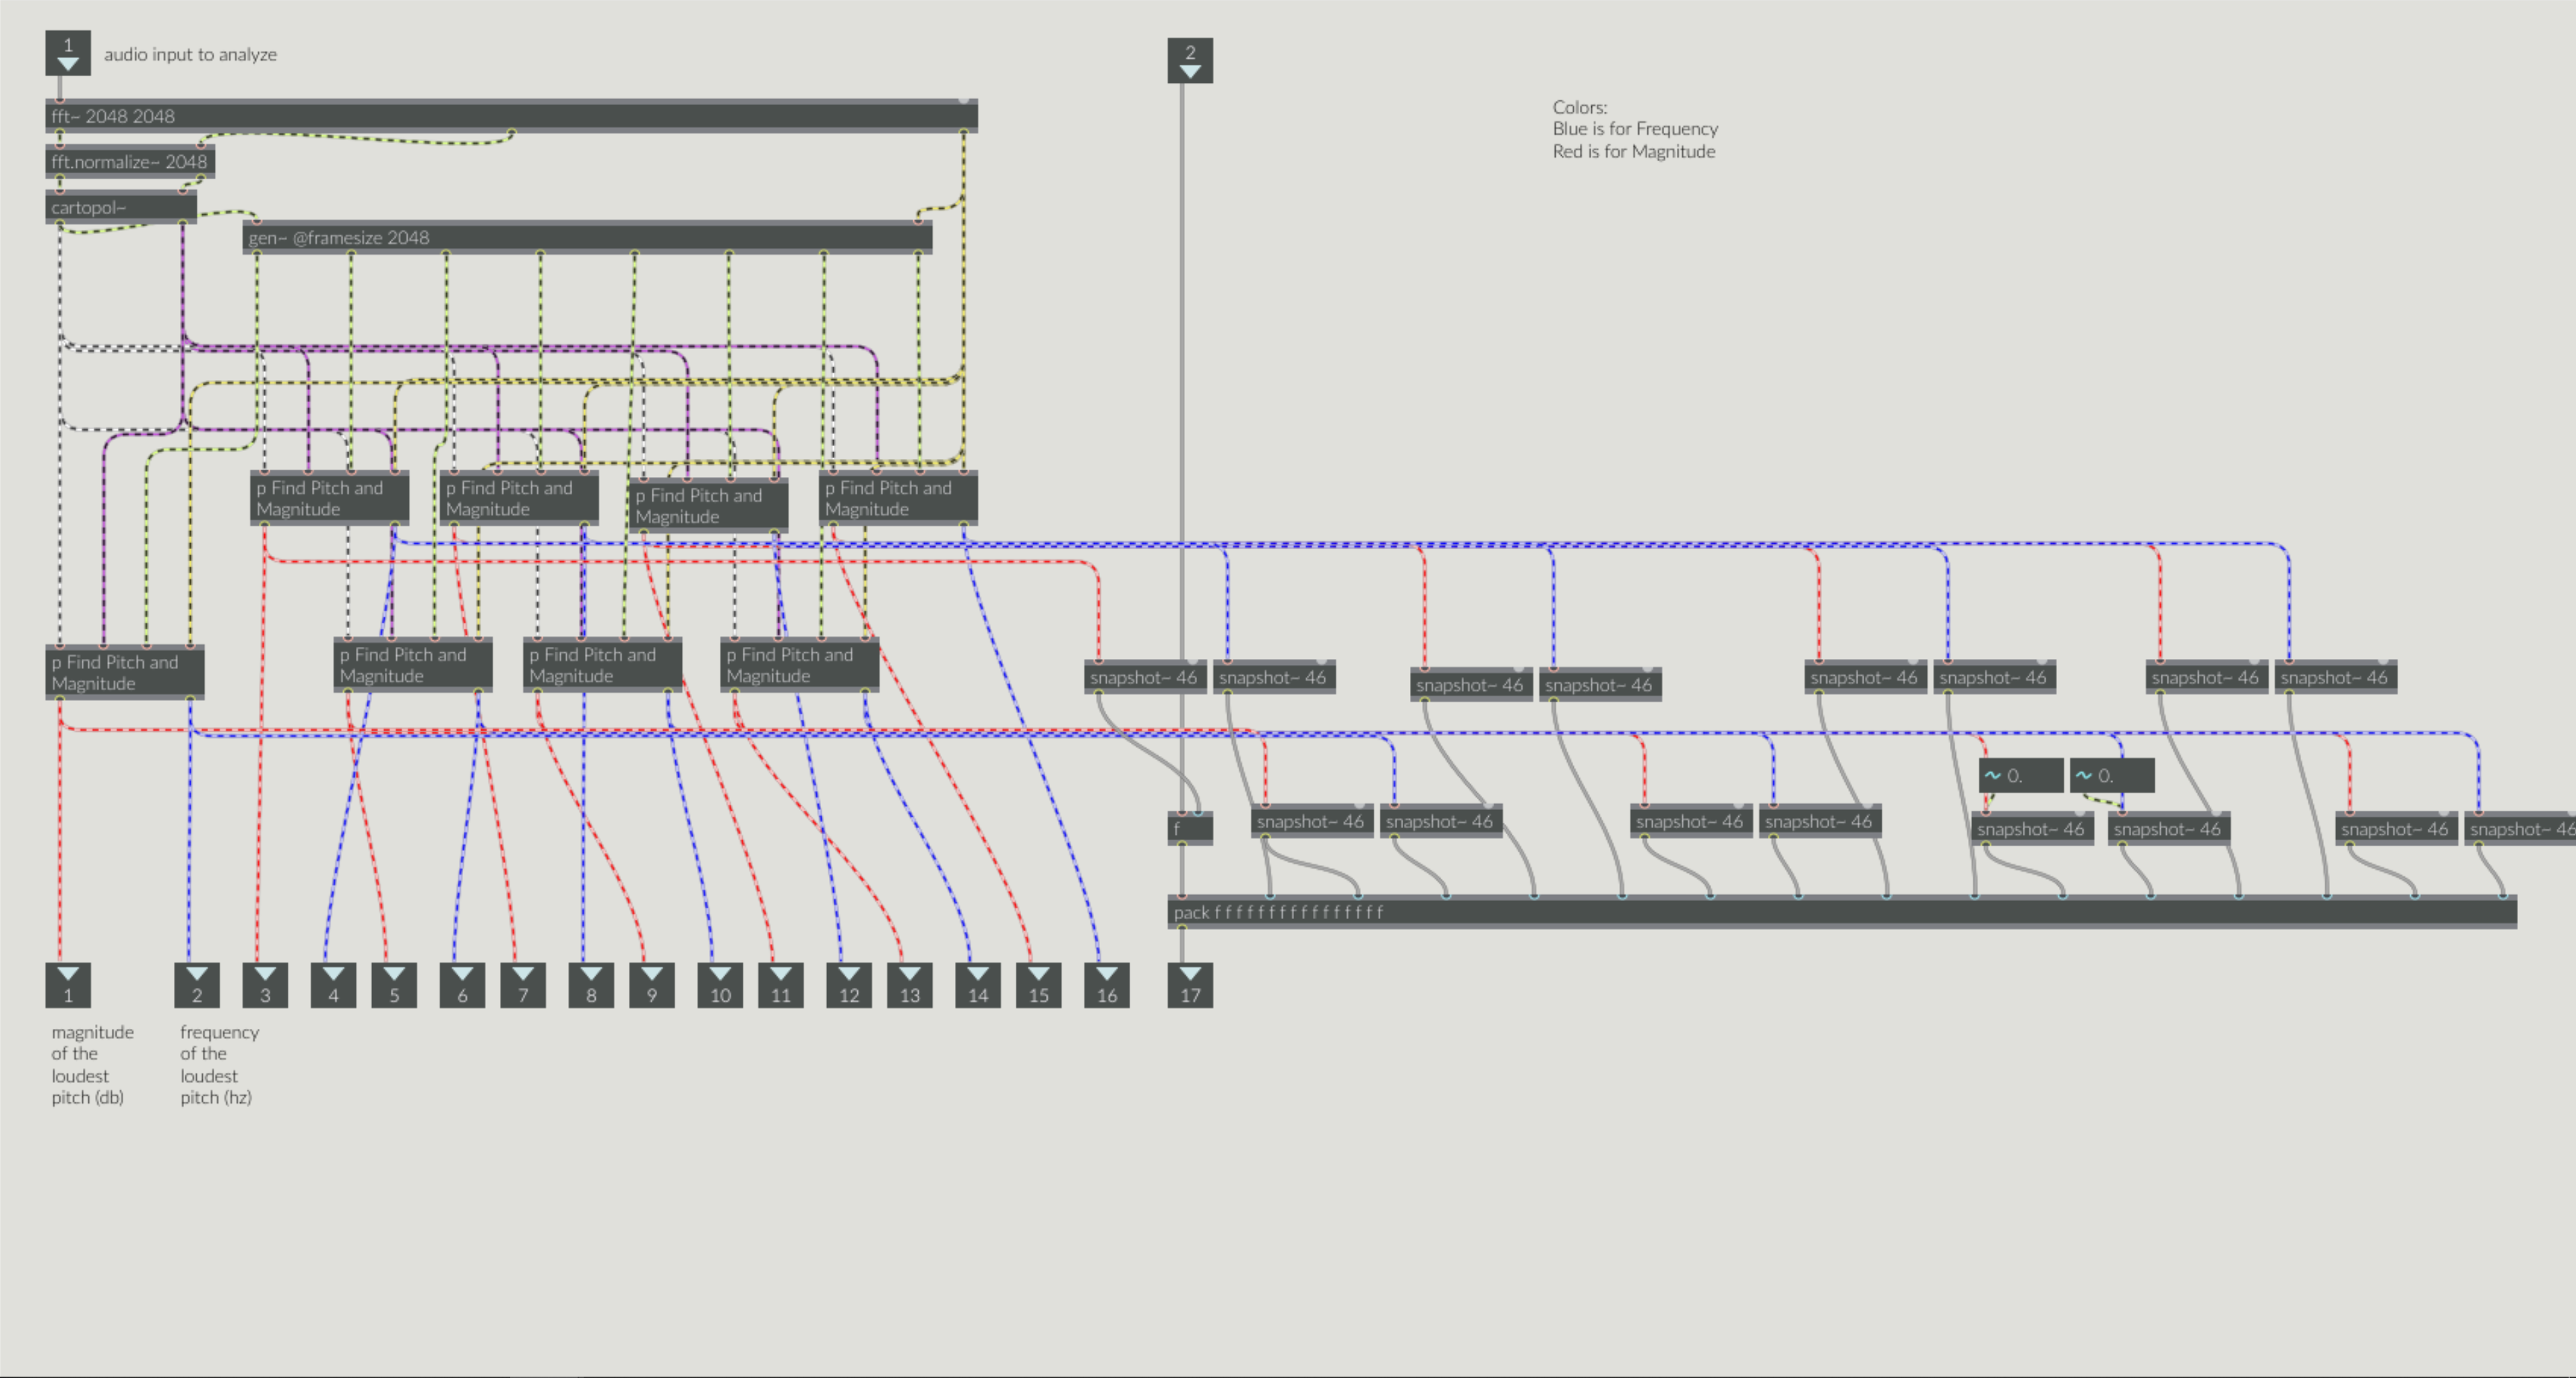
\includegraphics[width = \textwidth]{Graphs/MultipleTrack.png}
        \caption{Multiple Pitch tracking}
        \label{Analysis}
    \end{figure}

Afin de construire au mieux le patch, il est important de noter que la taille de la fenêtre affecte la qualité de la détection de la fréquence. La taille de la fenêtre influence la résolution temporelle ou fréquentielle de la représentation du signal. La résolution de fréquence peut être augmentée en modifiant la taille de la FFT, c'est-à-dire le nombre de segments de la fenêtre d'analyse. En particulier, la taille des bins correspond simplement à la moitié de la fenêtre d’analyse. La dispersion des fréquences est définie comme la division du SR par la taille de la fenêtre\footnote{Coralie Diatkine, \textit{AudioSculpt 3.0 User Manual}, 2011. \nocite{Audiosculpt}}.

    \begin{equation*}
        Frequency \; Range = \frac{SR}{Window \; Size}
    \end{equation*}

\section{Le vocodeur de phase}

Le vocodeur de phase est utilisé à l'origine pour la transposition de la hauteur et la modification de la vitesse de lecture. Pareillement, nous allons construire notre vocodeur de phase sur le modèle de base, puis nous proposerons quelques modifications. Le vocodeur de phase est étiqueté sous traitement spectral et va donc être stocké dans un objet \textit{pfft}$\thicksim $. Notre modèle est basé sur le vocodeur de phase par Dudas et Lippe\footnote{Richard Dudas et Cort Lippe, \textit{The Phase Vocoder}, 2006. \nocite{DL07} \nocite{DL06}}.

Pour accéder à un son directement dans l’objet \textit{pfft}$\thicksim$, il faut éviter d'utiliser les préréglages du  \textit{pfft}$\thicksim $. Par conséquent, nous allons éviter d'utiliser l'objet \textit{fftin}$ \thicksim $ à la place, nous allons utiliser un objet \textit{fft}$\thicksim $ dans un sous-patch. La seule différence est que les paramètres des objets \textit{fftin}$\thicksim $ et \textit{fftout}$\thicksim$ sont contrôlés directement à partir de l'objet  \textit{pfft}$\thicksim $ et que les entrées et sorties sont les premier et dernier objets. Pour construire un vocodeur de phase, nous devons traiter le son avant d'appliquer la transformation de Fourier. Pour comprendre la procédure on pourrait suivre le patch fourni dans la figure \ref{Phasevocoder}.

Le raisonnement derrière cette logique se repose sur le cœur du vocodeur de phase pour l'étirement sonore et le changement de la hauteur. Le vocodeur de phase nécessite une lecture indépendante du son à transformer pour chaque superposition de la FFT. Chaque image sonore de la lecture doit être synchronisée avec son image sonore respective de la FFT. Par conséquent, une seule copie du son ne peut pas être lancée dans un objet \textit{fftin}$\thicksim$, mais plutôt dans un objet \textit{fft}$\thicksim$. L'objet \textit{fft}$\thicksim$ exécute une FFT à spectre complet (c'est-à-dire en miroir), donc \textit{fft}$\thicksim$ peut fonctionner en synchronisation avec les images consécutives de la FFT traitées dans l'objet \textit{pfft}$\thicksim$ mais il est nécessaire de faire quelques modifications sur l'objet \textit{pfft}$\thicksim$ pour qu'il se comporte de la même manière.

Tout d'abord, l'objet \textit{pfft}$\thicksim$ doit traiter des images sonore de la FFT à spectre complet, au lieu de l'image spectrale par défaut qui correspond à la moitié de la taille de la FFT (jusqu'à la moitié de la fréquence de Nyquist). Cela peut être réalisé en ajoutant un cinquième argument non nul à l'objet \textit{pfft}$\thicksim$. Comme l'argument du spectre complet est le cinquième argument, nous devons fournir tous les autres arguments avant lui, y compris le quatrième argument (la position ou la FFT s’exécute) qui sera défini par défaut par zéro.

Ensuite, puisque les objets \textit{fftin}$\thicksim$ et \textit{fftout}$\thicksim$ effectuent le calcul de la FFT à la phase zéro par rapport à la FFT (le premier échantillon de la fenêtre envoyée au FFT est le milieu de la fenêtre), et les \textit{fft}$\thicksim$ et \textit{ifft}$\thicksim$ objets exécutent la FFT déphasée de 180 degrés, il faut assurer que tous les objets \textit{fftin}$\thicksim$ et \textit{fftout}$\thicksim$ du patch ont le même décalage de phase FFT utilisé dans les objets \textit{fft}$\thicksim$.

Cela peut être accomplie en spécifiant un déphasage par rapport aux objets \textit{fftin}$\thicksim$ et \textit{fftout}$\thicksim$. Une valeur de phase de $0.5$ signifie un déphasage de $180$ degrés, donc c'est la valeur préférable dans ce cas. Bien que, l'objet \textit{fftin}$\thicksim$ ne soit pas voulu, l'objet \textit{fftout}$\thicksim$ peut pratiquement être utilisé comme sortie pour l'objet \textit{pfft}$\thicksim$. Le fenêtrage automatique dans l'objet \textit{fftout}$\thicksim$ devrait se comporter comme le fenêtrage manuel avec les objets \textit{fft}$\thicksim$.

Dans cette version du vocodeur de phase, on va utiliser un son pré-déterminé. Cela veut dire qu'on utilisera un enregistrement et on le stockera dans un objet \textit{buffer}$\thicksim$. Le \textit{buffer}$\thicksim$ doit être accessible à deux endroits. Premièrement, à l'emplacement de l'image sonore de la FFT actuelle et, en deuxième lieu, à l'emplacement de l'image FFT précédente du \textit{buffer}$\thicksim$. Il est possible d'utiliser soit l'objet \textit{index}$\thicksim$ ou l'objet \textit{play}$\thicksim$\footnote{L'objet \textit{play}$\thicksim$ est utilisé comme interface de lecture de l'objet \textit{buffer}$\thicksim$. \textit{play}$\thicksim$ joue des samples en accord d'un offset parmi le buffer.} pour accéder au \textit{buffer}$\thicksim$. Lorsqu'on précise la position de la transformation Fourier en durée courte manuellement, on doit trouver un système pour préciser le décalage de la fenêtre dans notre \textit{buffer}$\thicksim$.

La solution dans cette problématique est d'utiliser deux objets \textit{fft}$\thicksim$ parallèles avec un décalage d'un quart, pour un chevauchement de $25 \%$. Un tel système permettra de calculer l'image actuelle de chaque index de la fenêtre en comparaison de l'index correspondant de la fenêtre précédente, comme cela a pu être fait dans le patch du pitch tracking. Le décalage est calculé pour une distance d'un quart puisqu'on prend en compte le paramètre du chevauchement. L'objet \textit{frameaccum}$\thicksim$ dans ce cas remplace la séquence des objets \textit{phasewrap}$\thicksim$, et normalisation entre $\pi$ et $-\pi$ qu'on a construit dans le patch du pitch tracking.

Pour la synchronisation du buffer on utilise un objet \textit{count}$\thicksim$ au paramètre $0$, la taille du fenêtrage, $1$ et $1$. On peut ainsi stocker la valeurs de l'échantillon exact au quelle la fenêtre de la FFT commence à la fois, ainsi que la position actuelle en durée totale du son. Chaque fois que le compteur se réinitialise à zéro, un objet \textit{sah}$\thicksim$ permet à la valeur de passer, dont on en déduit le premier sample de la FFT. En ajoutant les valeurs du compteur, on peut en déduire la position actuelle sur le fichier sonore. La valeur de la position sur le fichier nous permet de jouer le fichier à partir d'un objet \textit{play}$\thicksim$. 

On rappelle la formule du vocodeur de phase : 

    \begin{equation*}
    Phase \; Vocoder \; = \; \sum_{n=0} ^{N-1} h_a(n) \; x(n + uR_a) \; e^{-j \omega \frac{n}{N}} \vspace{0.5cm} 
    \end{equation*}
Dans la formule ci-dessus, on peut voir qu'il y a un fenêtrage correspondant, marqué $h_a(n)$. Pour simplifier, on va substituer avec quelques paramètres réels. On remplace $N$ par une taille de la fenêtre à $1024$ échantillons. On établit un décalage de 4 fois par fenêtre, donc $uR_a = (\frac{1}{4} * 1024)_a$ pour l'index $a$ de la fenêtre précédente.  
    \begin{equation*}
    Phase \; Vocoder \; = \; \sum_{n=0} ^{1023} h_a(n) \; x(n + 256_a) \; e^{-j \omega \frac{n}{1024}} \vspace{0.5cm} 
    \end{equation*}
À partir de cette formule, on peut identifier les éléments qui la reproduise dans le patch Max. La fonction, correspondant à la phase de l'analyse, contient la somme des échantillons du signal qui appartiennent à la taille de la fenêtre de la FFT, plus des échantillons qui appartiennent $\Sigma_n (x_n) $ à la fenêtre décalée par la taille du \textit{hop}, $uR_a$. Les échantillons sont multipliées, par une fenêtrage $h_a(n)$ et ensuite par la formule d'Euler qui équivaut à la transformation de Fourier.

    \begin{figure}
        \centering
        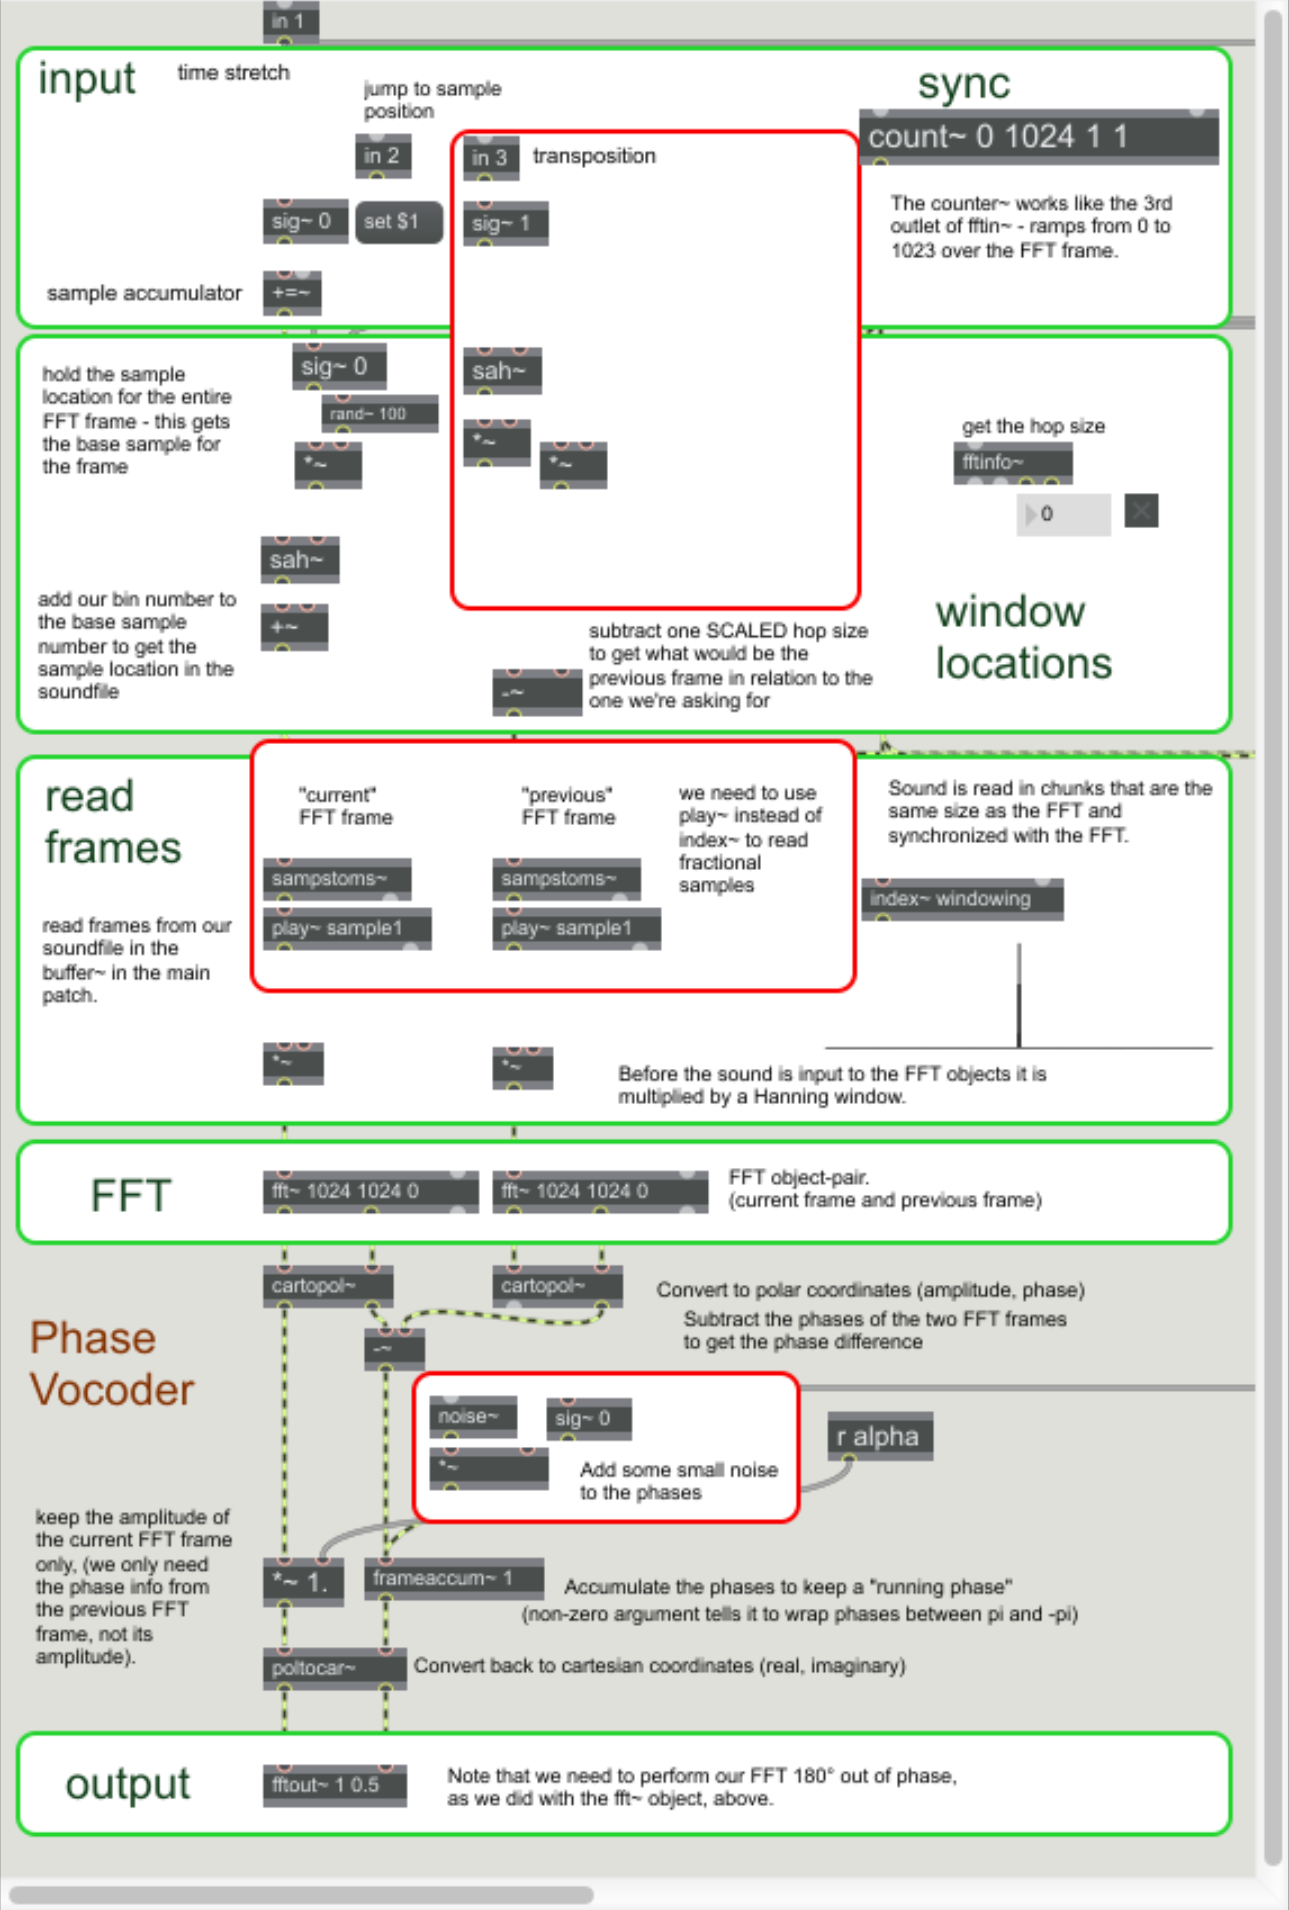
\includegraphics[width = \textwidth]{Graphs/PhaseVocoder.png}
        \caption{Le vocodeur de phase}
        \label{Phasevocoder}
    \end{figure}
    
Nous pouvons voir qu'une fonctionnalité de fenêtrage est inclu à la fois dans la formule et dans le patch présenté. Au lieu d'utiliser une fenêtre par défaut de l'objet \textit{fft}$\thicksim $, nous allons utiliser un buffer fixé de taille $ N $. En utilisant l'objet \textit{count}$\thicksim $ avec l'aide de l'objet \textit{index}$\thicksim$ \footnote{L'objet \textit{index}$\thicksim $ est utilisé pour lire un objet $ buffer \thicksim $ dans un exemple d'index piloté par signal sans interpolation sur la sortie.}, pour accéder à chaque échantillon, on multiplie le son de l'entre par les valeurs du fenêtrage avant d'effectuer de la FFT.

\subsubsection{Filtre Gabor}

Dans la section 2, nous avons présenté le filtrage de Gabor. Dans cette section, nous allons créer un filtre Gabor personnalisé. La formule de Gabor normalisée permet de modifier la courbe de la fonction gaussienne tout en conservant les constantes de valeurs maximales et minimales. Cette fenêtre gaussienne faite sur mesure est présentée en figure \ref{windowing}.

Nous utilisons un objet \textit{uzi}\footnote{Envoyer instantanément le nombre de \guillemotleft bangs \guillemotright qui ont été définies dans la position de l'argument de l'objet.} avec argument la taille de la fenêtre FFT, suivie de l'expression effectuant une courbe gaussienne normalisée. Ensuite, nous l'envoyons dans le buffer nommé \guillemotleft windowing \guillemotright à l'aide de l'objet \textit{peek}$ \thicksim $ \footnote{L'objet \textit{peek}$ \thicksim $ est utilisé pour lire et écrire des de valeurs des échantillons dans un \textit{buffer}$ \thicksim $ }. Bien sûr, dans ce cas, le filtre de Gabor n’est pas directement exécuté pendant la FFT, mais juste avant. En utilisant ce filtrage, nous pouvons librement chevaucher des fenêtres et éviter des artefacts.
    
    \begin{figure}
        \centering
        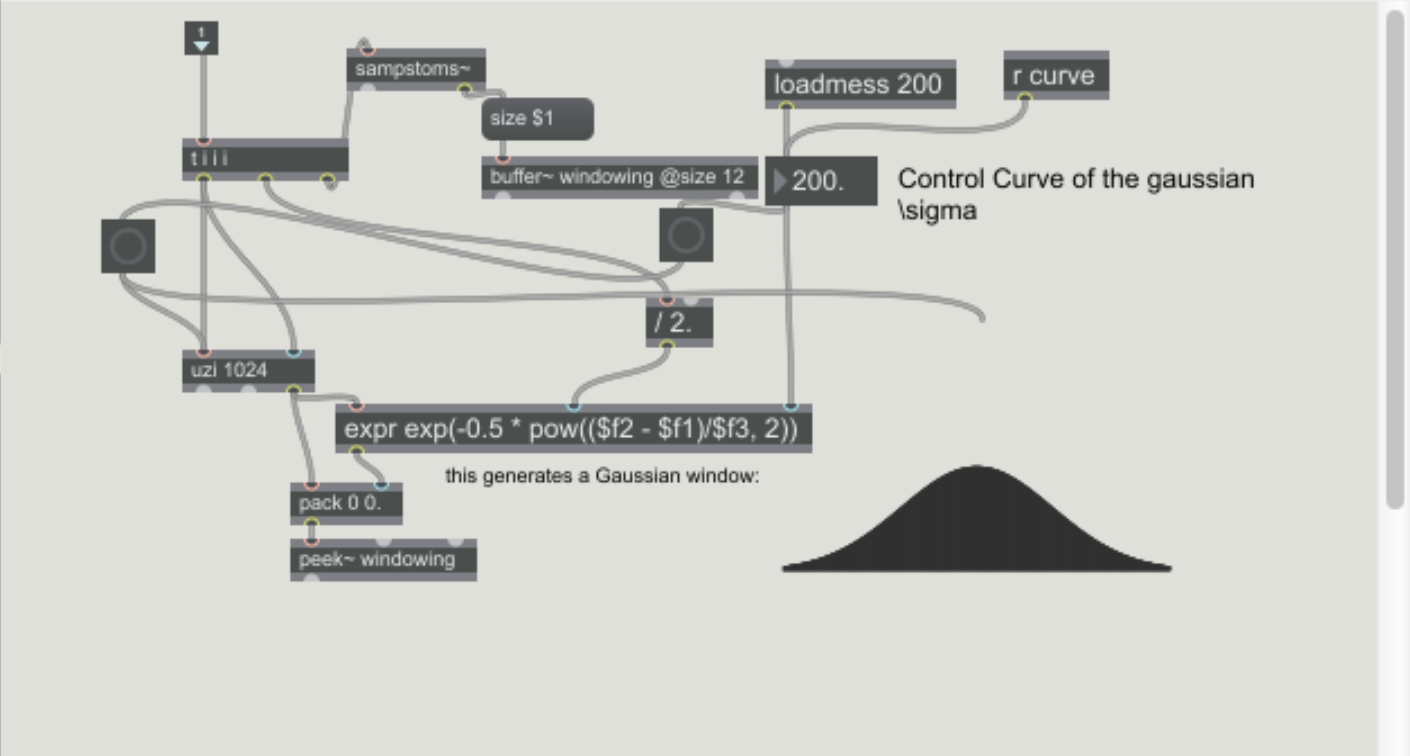
\includegraphics[width = \textwidth]{Graphs/windowing.png}
        \caption{Fenêtrage gaussien}
        \label{windowing}
    \end{figure}

\subsubsection{Transposition de la hauteur}

    Pour appliquer la transposition de la hauteur avec le vocodeur de phase, il convient de modifier le facteur de la hauteur tout en modifiant simultanément la fréquence d'échantillonnage. Par exemple, afin de transposer un son d'une octave plus basse, nous devons reproduire le son à une vitesse deux fois moins rapide, tout en doublant le SR. En utilisant cette méthode, il est possible de changer la hauteur en modifiant la vitesse de lecture.

    Pour utiliser cette méthode, nous utilisons des valeurs MIDI standard traduites en fréquence et adaptées au chevauchement des fenêtres. L'utilisateur peut ensuite saisir la valeur dans un piano midi virtuel, facilitant ainsi la manipulation. Par défaut, la note midi Do avec la valeur 60 est la hauteur standard. Ensuite, la hauteur change en fonction de l'intervalle en fonction de la valeur par défaut. Par conséquent, la valeur Do une octave inférieure dans le piano midi virtuel correspond à une octave de transposition inférieure à la hauteur originale du son.

    À l'intérieur du vocodeur de phase, le décalage de hauteur est traduit par le saut d'échantillons ou le sur-échantillonnage de l'objet  \textit{count}$\thicksim $. Bien sûr, augmenter le SR n'est pas une solution valable, nous avons donc choisi de prendre une portion plus petite ou plus grande du \textit{buffer}$\thicksim $ correspondant à la taille de la fenêtre. Une transposition vers le haut correspond au fait de prendre une fenêtre plus grande dans \textit{buffer}$\thicksim $ et de la lire à une vitesse plus rapide, tandis qu'un décalage de hauteur correspond à couper une plus petite partie de la variable \textit{buffer}$\thicksim $ et à la lire plus lentement.

    Pour cet exemple, nous utilisons un objet \textit{sah}$\thicksim $ pour nous assurer que la valeur de transposition est maintenue constante pour tous les bins pendant la FFT. Ensuite, nous multiplions par la valeur actuelle du compteur et nous ajoutons la valeur de sortie au nombre d'échantillons déjà lus pour obtenir l'emplacement souhaité du fichier. En ce qui concerne la fréquence initiale $ \omega $, le décalage individuel s’élève à:

    \begin{equation*}
        \Delta \omega(\omega) = \omega (\alpha - 1)
    \end{equation*}

    Où $ \alpha $ est le facteur de transposition et $ \Delta \omega $ la différence de fréquence. Cette technique impose une transposition de fréquence constante $ \Delta \omega $ à toutes les fréquences détectées de la FFT.

    L'implémentation Pitch Shifting peut être vue dans la figure. Quelques objets suffisent pour implémenter un décalage de hauteur sur le corps de base du vocodeur de phase.


\subsubsection{Modulation Temporelle}

    Comme il a été étudié à la section 2, modifier la vitesse de lecture tout en gardant la hauteur du pitch stable est l’opération inverse de la transposition de la hauteur. La lecture peut être contrôlée en prenant en compte le facteur de chevauchement des fenêtres FFT. On peut diviser par le facteur du chevauchement et ajouter le pourcentage de la lecture souhaitée. À l'intérieur du vocodeur, la valeur factorisée est ajoutée à l'accumulateur d'échantillons. Dans ce cas, la valeur de la vitesse de lecture est ajoutée sur la position de l'interprétation de chaque échantillon. Une lecture plus rapide peut enjamber des échantillons où une vitesse de lecture plus lente lit plusieurs fois chaque échantillon. La soustraction de la position précédente de chaque échantillon (la fenêtre de la FFT), fixe les déviations de fréquence. 

\section{Morphing spectrale}

La démonstration finale de ce chapitre est une implémentation du morphing spectral ou de la synthèse croisée spectrale. Pour accomplir cette technique, nous utilisons deux vocodeurs en phase parallèles et nous interpolons la phase et l’amplitude entre toute indice du bin. Pour comprendre la complexité computationnelle du morphing spectral, rappelons-nous qu'un vocodeur à phase simple utilise deux FFT parallèles décalées du facteur de fenêtre de recouvrement. Donc, si nous utilisons une fenêtre de 1024 échantillons et un facteur de chevauchement de 4, la première FFT commence en position $ 0 $ et la fenêtre parallèle en position d’échantillon $256$. Nous utilisons maintenant 4 FFT parallèles pour le morphing spectral. Cela fait une prix computationnelle relativement haute, mais il reste possible de le calculer avec les ordinateurs actuels.

Dans ce double vocodeur de phase, les sorties de l'objet \textit{cartopol}$ \thicksim $, la magnitude et la phase après l'analyse de Fourier, sont multipliées par le facteur d'interpolation de morphing. La phase est préalablement corrigée par une accumulation avec l'harmonique précédente et une petite quantité de bruit est ajoutée pour la naturalisation du résultât sonore. Nous séparons les canaux d’interpolation de magnitude et de phase. Ainsi, on peut préférer émettre, par exemple, l’amplitude du son source mais la phase du son cible.

La sortie de chaque son après l’interpolation est transformée en forme cartésienne et une FFT inverse est appliquée. Ainsi, nous obtenons un résultat sonore homogène. À ce stade, un certain nombre d'opérations d'édition peuvent être ajoutées, telles que la modélisation du bruit ou une interpolation variable par image, etc. Mais avant de plonger dans des modifications avancées, examinons d'abord les techniques d'interpolation.

L'interpolation est définie par défaut sur linéaire. Un simple code Javascript que nous avons implémenté crée une courbe linéaire. Les valeurs d'interpolation varient entre $ [0, 1] $. La valeur $ 0 $ correspond à une interpolation nulle, et par conséquent la magnitude ou la phase du son source est sortie. Une valeur de $ 1 $ restitue entièrement les caractéristiques du son target et omet le son source. Une courbe linéaire définit une méthode linéaire pour interpoler les sons. En allons plus loin, nous implémentons un certain nombre de courbes telles que exponentielle, logarithmique et, bien entendu, linéaire. Par conséquent, il existe différentes manières d'interpoler des sons en fonction de leurs composantes de fréquence ou de la magnitude de leurs composantes de fréquence. Toutes les interpolations varient entre la même intégrale $ [0, 1] $. Le code Javascript peut être consulté dans le bout de code ci-dessous.

La version du vocodeur de phase pour le morphing spectral est montrée dans la figure \ref{Morphing}. Il existe deux buffers, un pour la source et un pour le son target. Le fenêtrage gaussien pour du filtrage Gabor, avec une courbe normalisée à distance, est aussi paramétrable dans la plateforme. Un bouton d’interpolation pour la phase et un bouton pour l’interpolation de la magnitude contrôlent les facteurs d’interpolation pour le morphing et une factorisation du bruit pour la naturalisation de la phase sont mis en œuvre.

    \begin{figure}
        \centering
        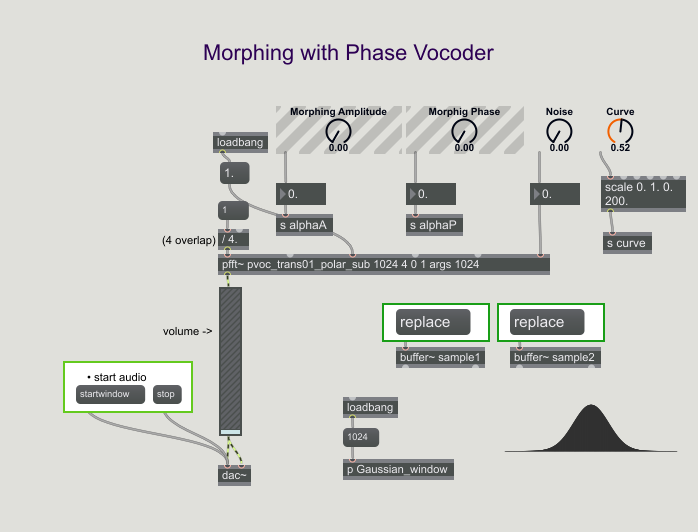
\includegraphics[width = \textwidth]{Graphs/SoundMorphing.png}
        \caption{Morphing en temps réel}
        \label{Morphing}
    \end{figure}


\noindent\begin{minipage}{\textwidth}
\lstinputlisting[language=Java]{Expondential.js}
\end{minipage}
\chapter{Implémentations artistiques}

\label{ch:Implémentations aristiques}

\section{Introduction}

Cette section conclut un point de vue artistique sur les aspects abordés dans les chapitres précédents. À partir de la transformation de Fourier en vocodeur de phase et en passant au morphing par des interprétations artistiques des patchs techniques mis en œuvre.

L'objectif de ce chapitre est de soutenir l'idée que l'analyse et la re-synthèse spectrales, et donc en expansion, le développement du signal musical  sont utiles aux scientifiques et aux artistes. En effet, les détails techniques antérieurs sont utilisés à des fins artistiques et esthétiques. Les exemples suivants consistent en une expérimentation personnelle et une interprétation du matériel technique déjà présenté.

\section{Le vocodeur de phase - \textit{Une capacité sans fin}}

\subsection{Super Phase Vocoder}

Dans le but de combiner plusieurs techniques du vocodeur de phase, nous avons implémenté un \guillemotleft \textit{super} vocodeur de phase\guillemotright . Cet outil spectral comprend l'étirement temporel, le freeze temporel, le décalage de hauteur, le morphing et d'autres effets bénéficiant de la fonction élémentaire du vocodeur de phase.

Le graphe \ref{FirstMorphingTry} presente le patch de contrôle de tous les paramètres du vocodeur de phase. Cette version du vocodeur de phase contient tous les effets étudiés dans les sections précédentes. Il n'y a pas quelque chose de particulièrement différent du vocodeur de phase de base pour le morphing apart quelques fonctionnalités de plus. Il est naturel de rechercher une fonctionnalité plus large pour le même outil. En suivant cette raisonement, nous avons implémenté tous les effets de base dans un seul patch. Les maths ici ne sont pas intéressants à analyser car ils ont tous été vus auparavant. Les détails les plus cruciaux se trouvent dans la séquence de tous les effets visibles dans figure \ref{SuperPhaseVoc}.

Dans le patch principal, vous pouvez voir deux pianos virtuels de contrôle permettant de modifier la hauteur de chaque son séparément. Idéalement, ce système devrait être automatique. Il faut estimer la fréquence de chaque son et corriger à mi-chemin la hauteur du son pour qu'il en soit de même. Une correction de hauteur intervient avant tout effet de morphing et n'affecte donc pas le résultat. Dans le patch principal, nous pouvons également trouver des commandes permettant de manipuler le filtre de Gabor, en ajustant les composantes de bruit de la phase qui, dans ce patch, sont identiques pour les deux sons. On peut également trouver des facteurs d’interpolation de magnitude et de phase pour le morphing, ainsi que la factorisation de la courbe, comme indiqué dans la section précédente. La dernière modification présentée dans ce patch est l'effet de \textit{freeze} qui contient les valeurs spectrales d'une seule fenêtre. Pour cet effet, deux types de filtrage sont également ajoutés pour modifier le timbre des spectres gelés.


\begin{figure}
\centering
\begin{subfigure}{\textwidth}
  \centering
  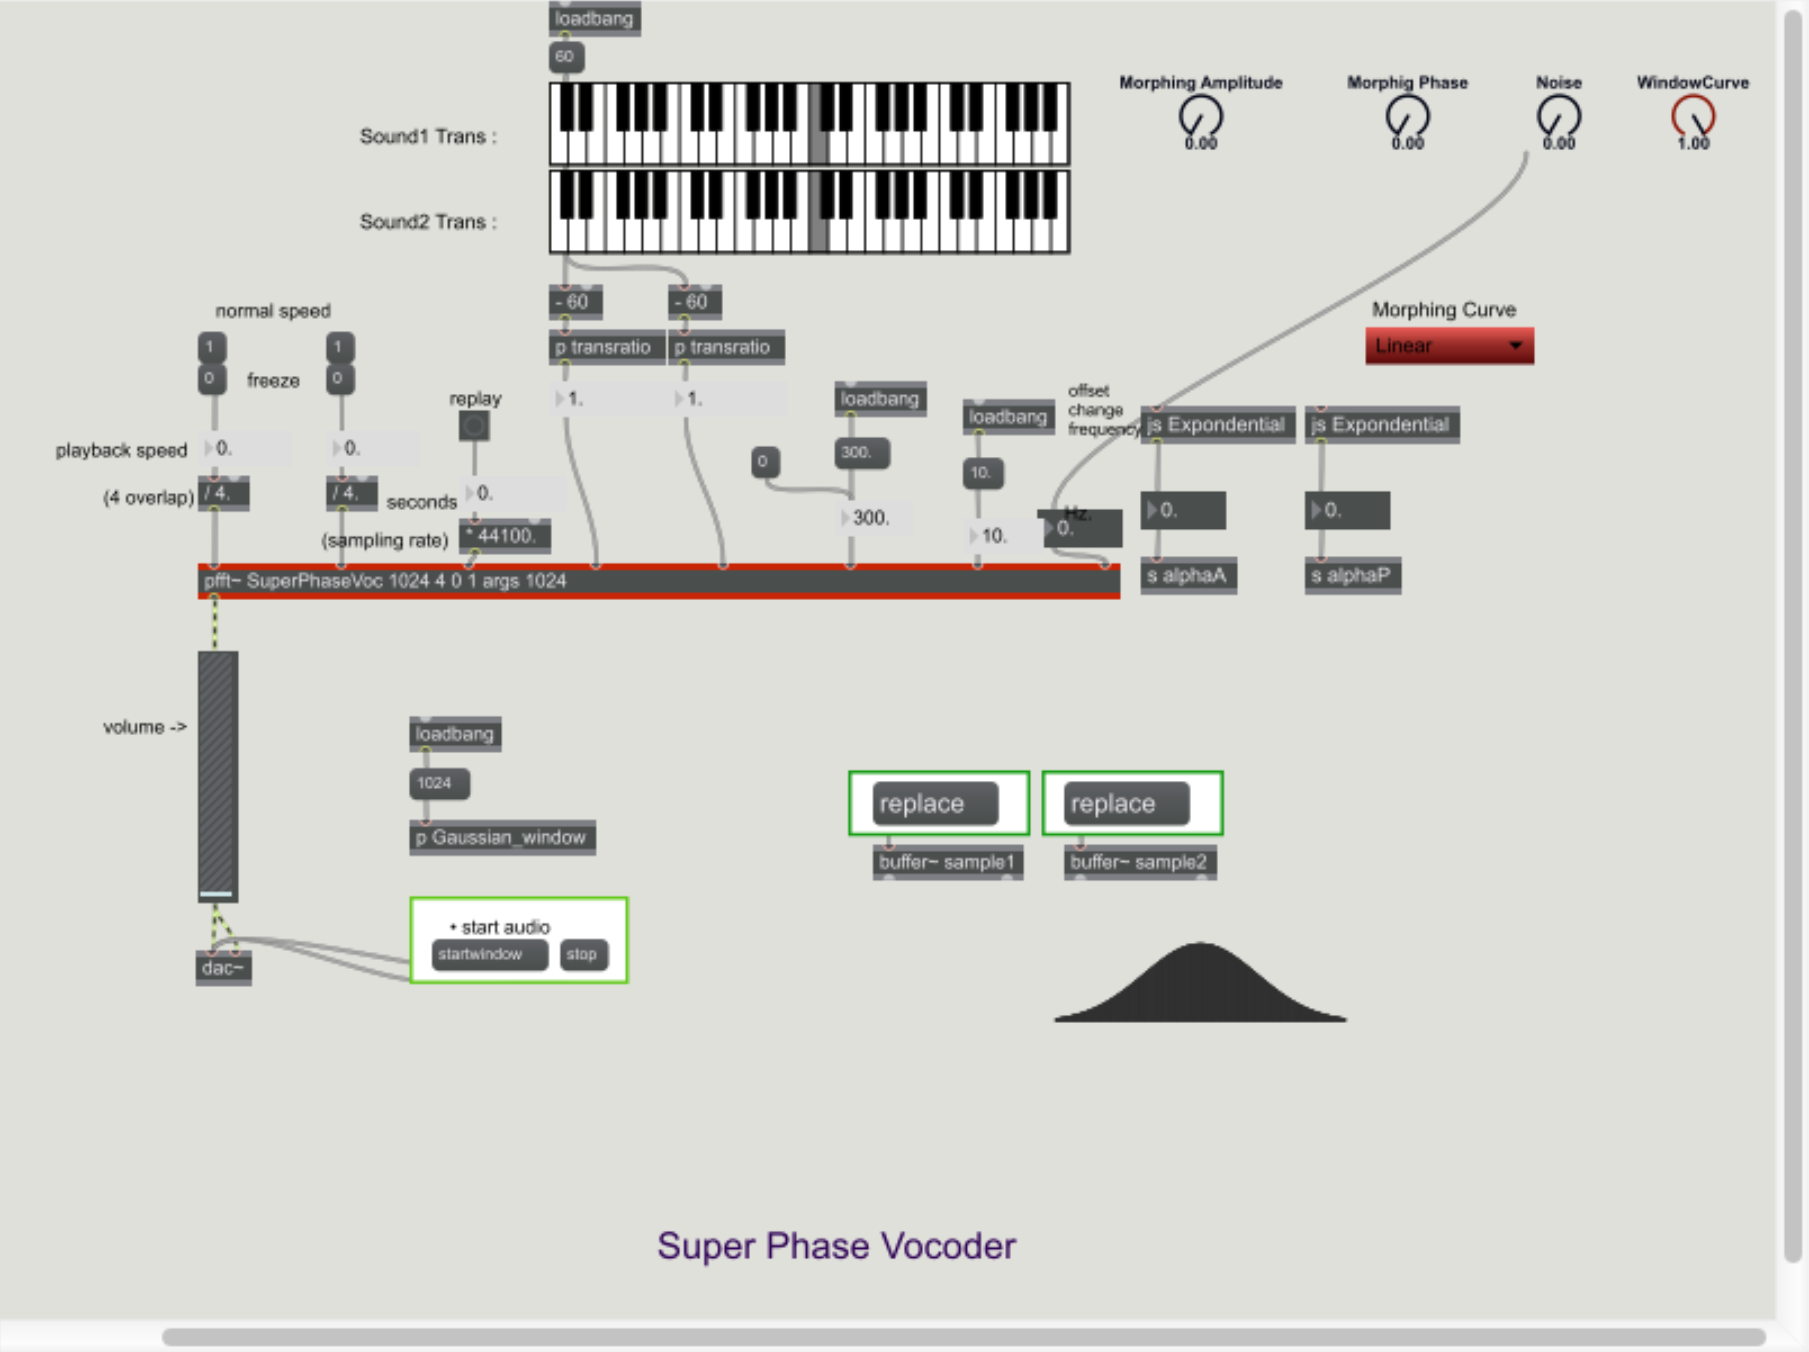
\includegraphics[width=.8\linewidth]{Graphs/FirstMorphingTry.png}
  \caption{Super Phase Vocoder I}
  \label{FirstMorphingTry}
\end{subfigure}

\begin{subfigure}{\textwidth}
  \centering
  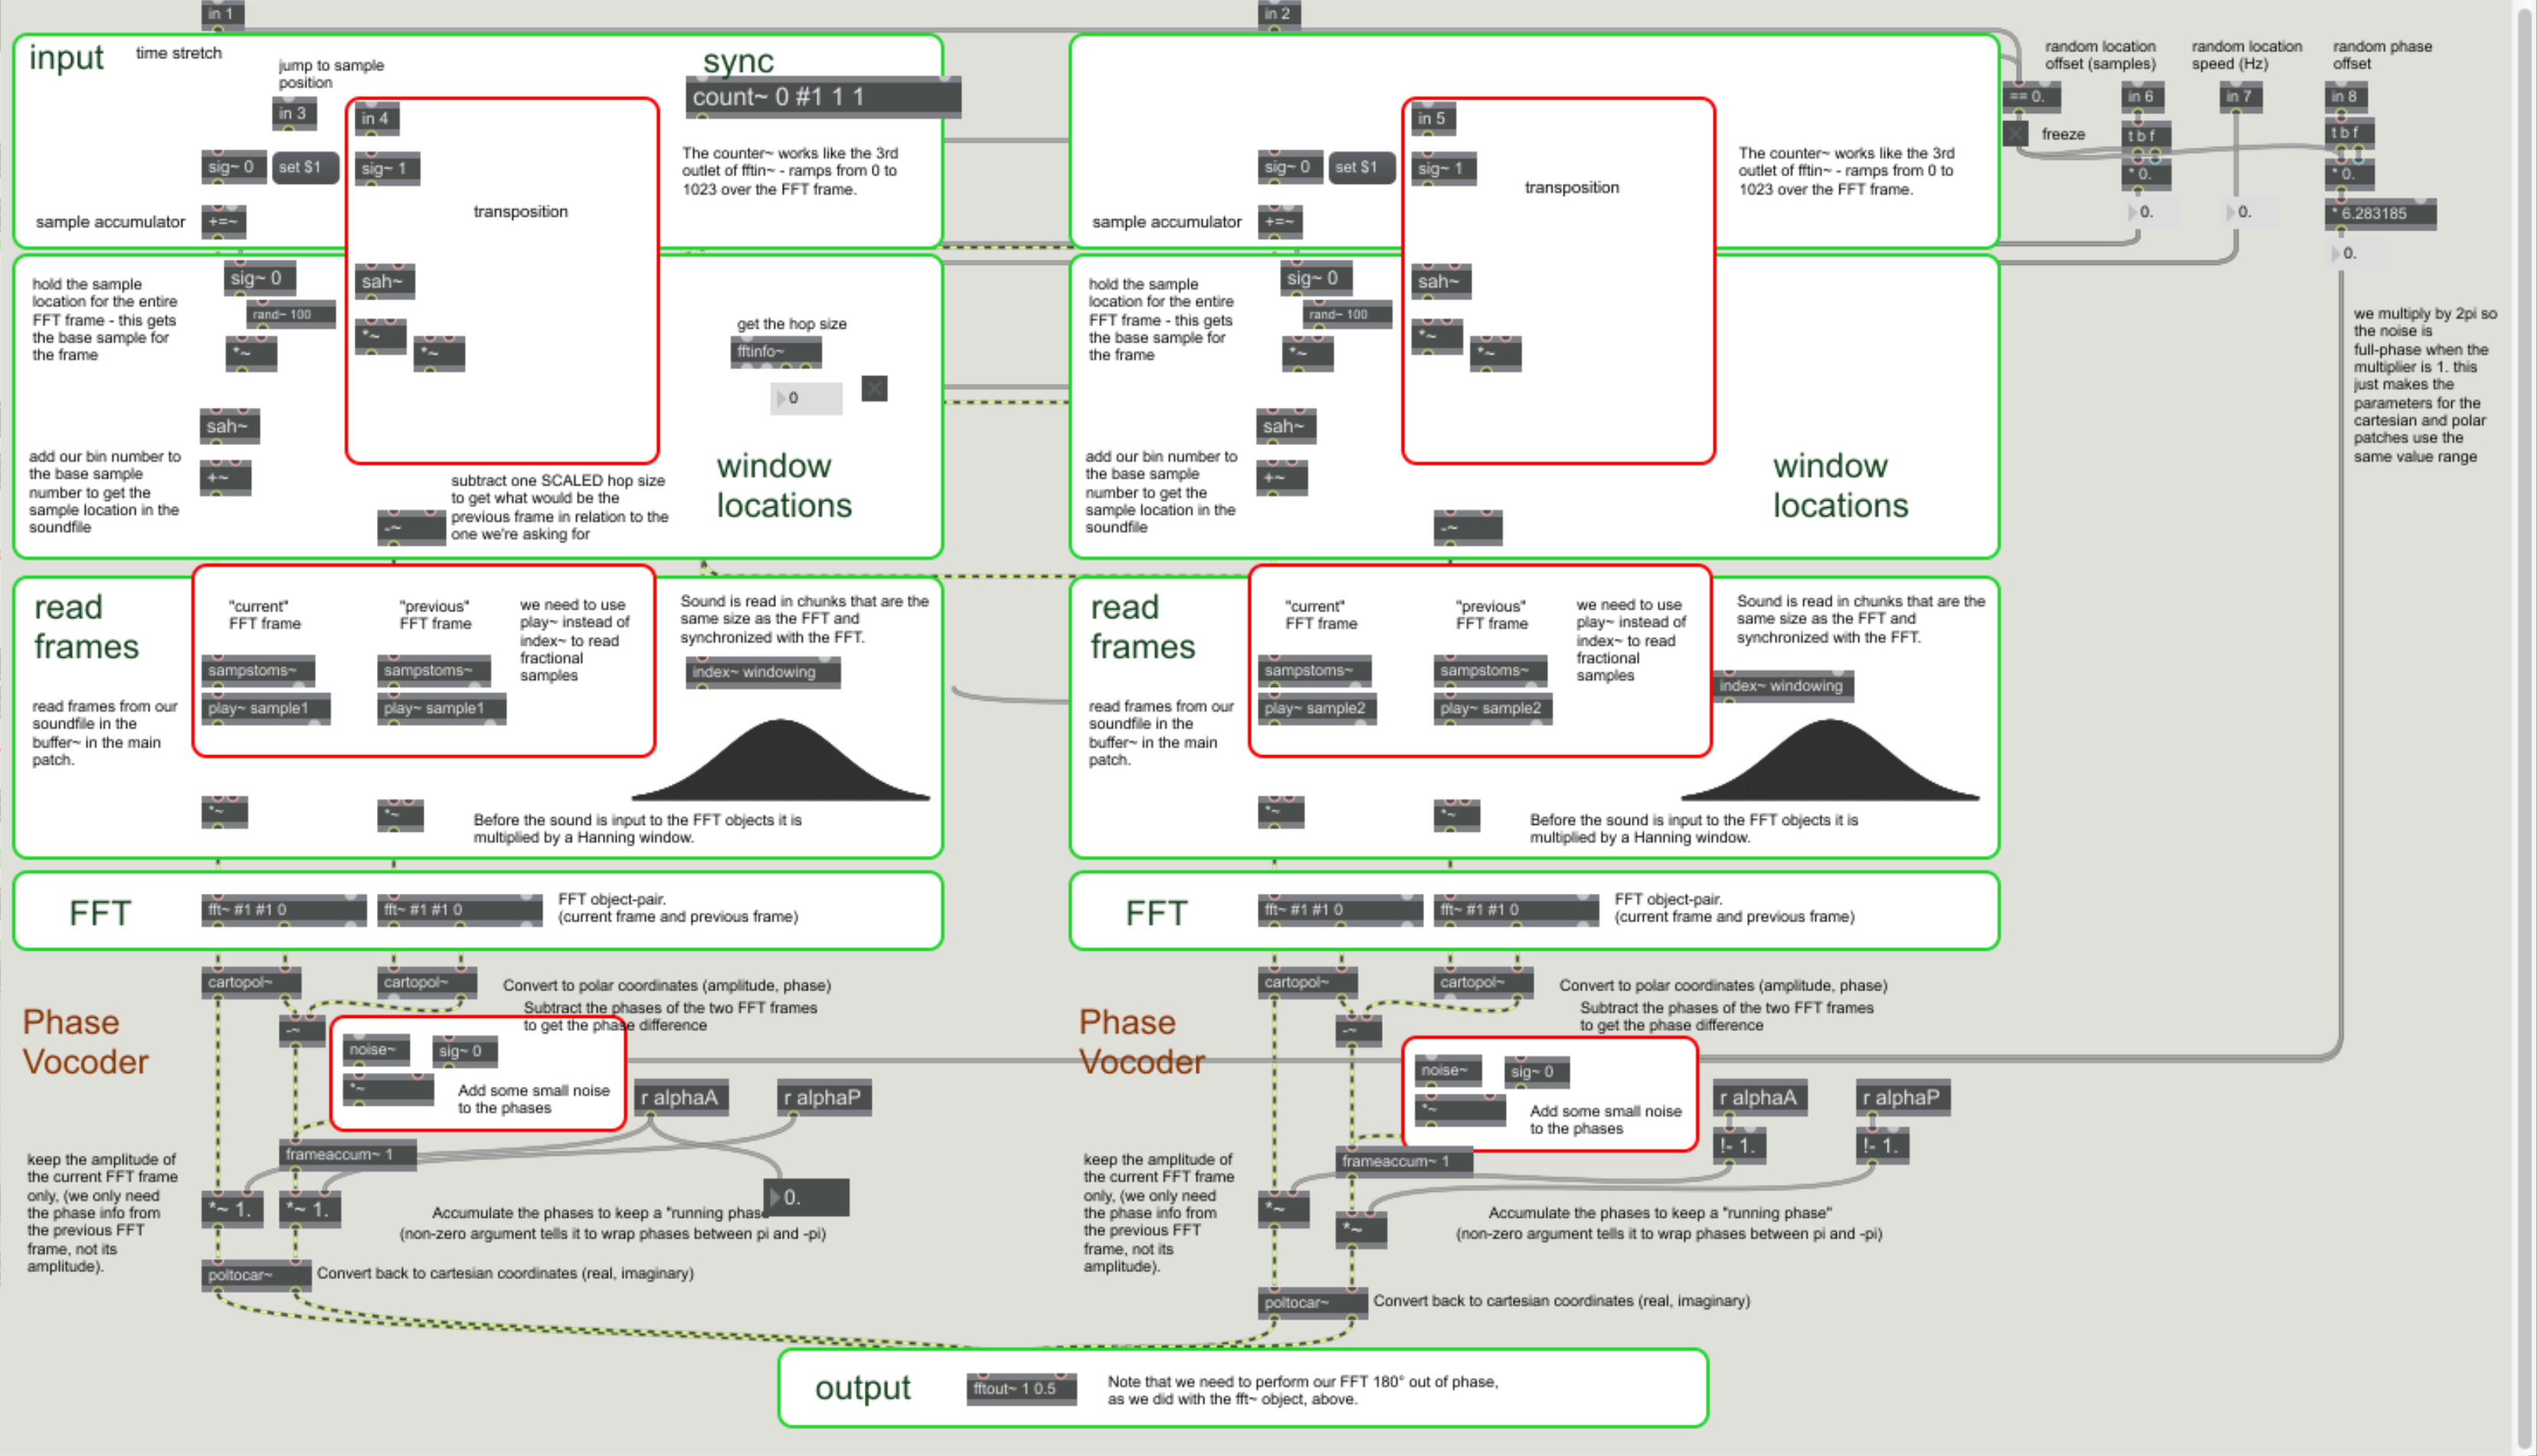
\includegraphics[width=.8\linewidth]{Graphs/SuperPhaseVoc.png}
  \caption{Super Phase Vocoder II}
  \label{SuperPhaseVoc}
\end{subfigure}
\caption{Super Phase Vocoder}
\label{PhaseVocoder}
\end{figure}

\subsection{Phase interference}
    Dans ce patch MaxMSP, nous étudions une modification des coordonnées polaires après l’étape de l’analyse. Nous ajoutons simplement un oscillateur de phaseur après la FFT et l’appliquons à chaque amplitude et phase corrigée de la fenêtre. De cette façon, l'identité du signal n'est pas modifiée, mais une fréquence oscillante interfère avec chaque index de la fenêtre FFT. La formule de cette modification est présentée ci-dessous par l'équation de synthèse.

\begin{figure}
  \centering
  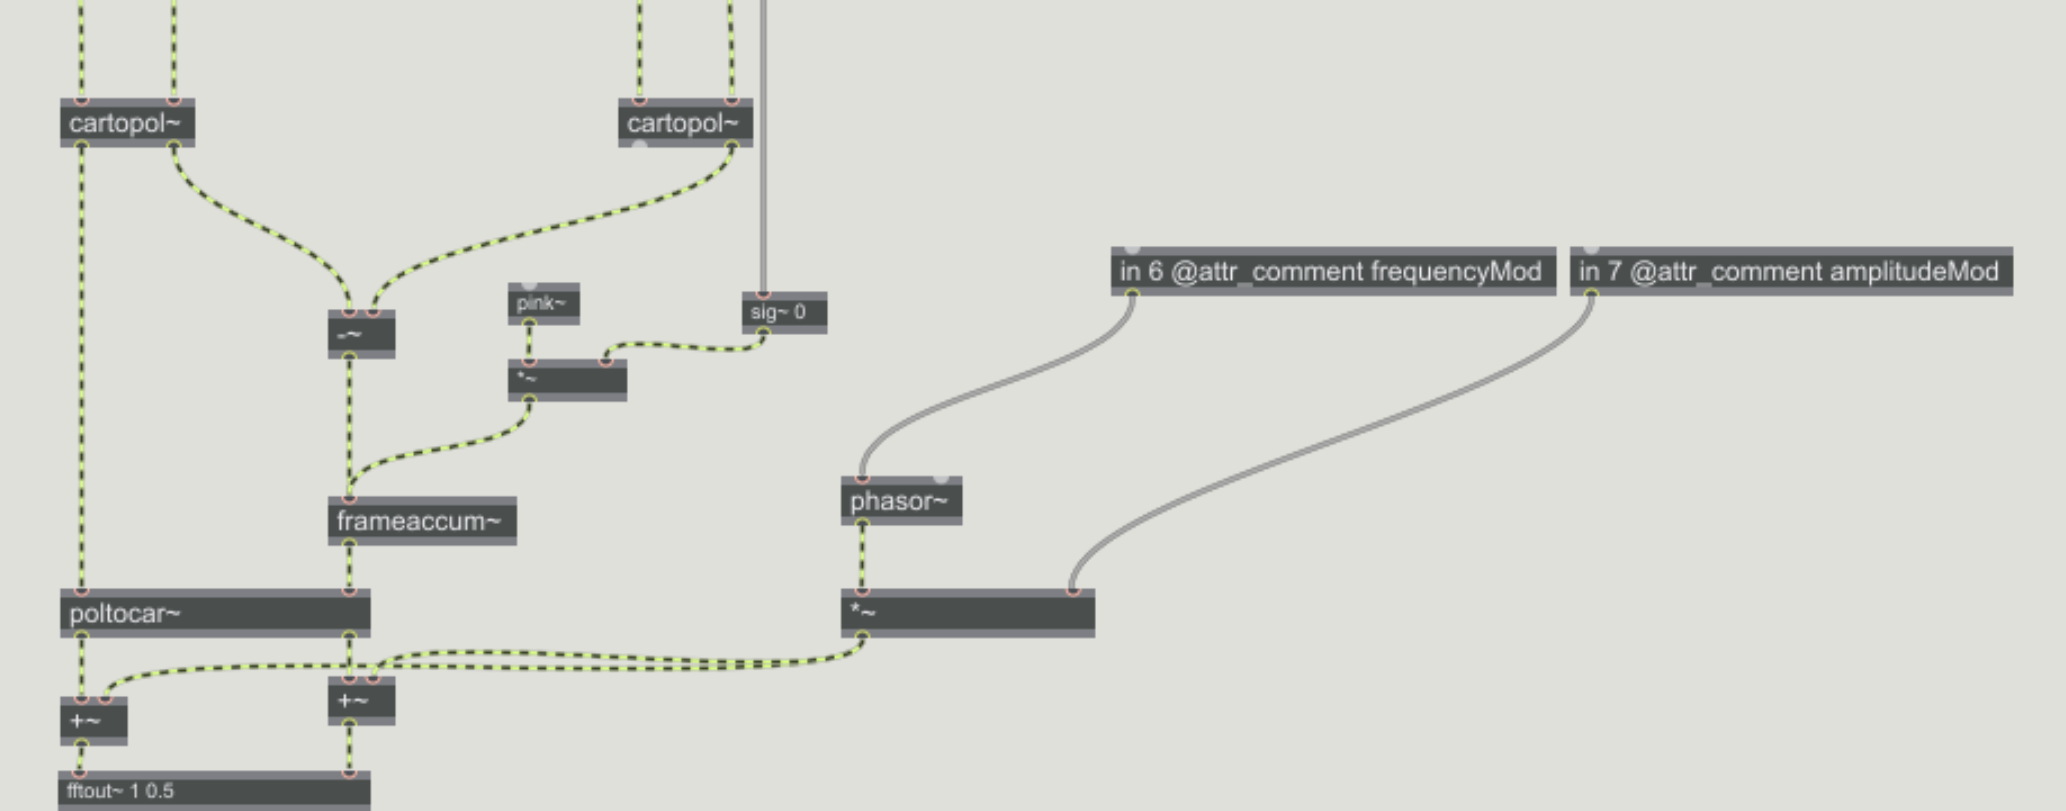
\includegraphics[width= 0.5 \textwidth]{Graphs/phasorInt.png}
  \caption{modulation \\ des coordonées polaires}
  \label{phasorInt}
\end{figure}

    \begin{equation}
      y(n, k) = \sum_{k=1}^K (A[n]+phi(n)) \; e^{j (\theta_k(n) +\phi(n)}
    \end{equation}
    
    Où $y (n, k)$ est le signal fenêtré après l'analyse. K est le nombre de sinisoides, $ A [n] $ est la magnitude instantanée, $ \theta $ est la phase instantanée et $ \phi (n) $ est le phaseur instantané donné par la formule:

    \begin{equation*}
        \phi(n) = n - floor(n)
    \end{equation*}

    Nous pouvons voir que le modèle sous-jacent de la FFT est utilisé pour représenter cette modification. D'autres modèles pourraient parfaitement décrire cet effet, mais dans cette version, il est plus direct. Dans la figure correspondante \ref{phasorInt}, nous pouvons voir le phaseur moduler la magnitude et la phase. La fréquence et l'amplitude du phaseur sont contrôlées dans le patch principal contenant l'objet pfft $ \thicksim $.

\subsection{Modulation au bruit}

\begin{wrapfigure}{r}{0.5\textwidth}
  \vspace{-20pt}
  \begin{center}
    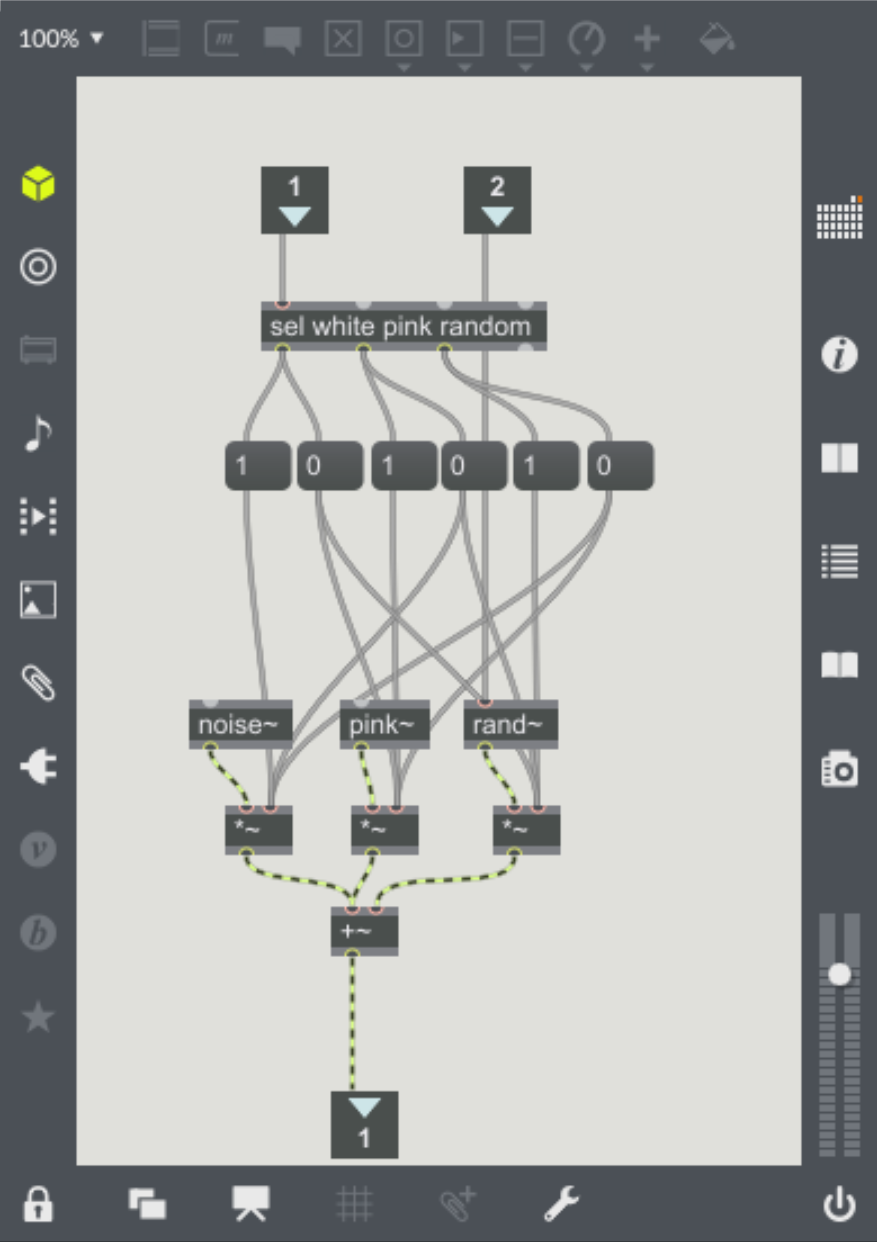
\includegraphics[width=0.48\textwidth]{Graphs/Noise_Select.png}
  \end{center}
  \vspace{-20pt}
  \caption{Selection du bruit}
  \vspace{-10pt}
\end{wrapfigure}

    Dans ce vocodeur de phase, nous étudions une modulation de bruit sur la composante de fréquence. Nous avons ajouté la composante de bruit et essayé différents générateurs de bruit tels que $ rand \thicksim $, pink-noise, white-noise et en même temps nous avons contrôlé le facteur d'amplitude de cette composante. Le sous-patch pour la sélection du bruit est visible dans la figure \ref{Noise_Select}. Un objet umenu fonctionne comme un stade de sélection pour l'utilisateur du maître transmettant ses valeurs au sous-patch pfft.

    La phase corrigée, par la fenêtre FFT de chevauchement, est multipliée par le facteur du bruit. Dans les dossiers sonores de cette thèse, on entend les différentes modulations de bruit, mais le résultat sonore n’est pas évident. Le facteur de bruit est utilisé pour la naturalisation du son car les fréquences continues pures ne sont pas produites dans les sons réels. Par conséquent, une petite correction de l'oscillateur de bruit ne donne pas un résultat strictement différent.

\subsection{Filtre aletoire sur la position du buffer$\thicksim$}

    Dans ce patch, nous modulons la position du tampon via un générateur de signaux aléatoires qui transmet ses valeurs au lecteur de la position du fichier. Pour être plus précis, nous filtrons les harmoniques de la FFT en produisant des nombres aléatoires pour chaque harmonique et en ne calculant l'harmonique $ k-$\ième que si le nombre aléatoire correspondant est inférieur à sa valeur d'index.

\begin{wrapfigure}{r}{0.5\textwidth}
  \vspace{-20pt}
  \begin{center}
    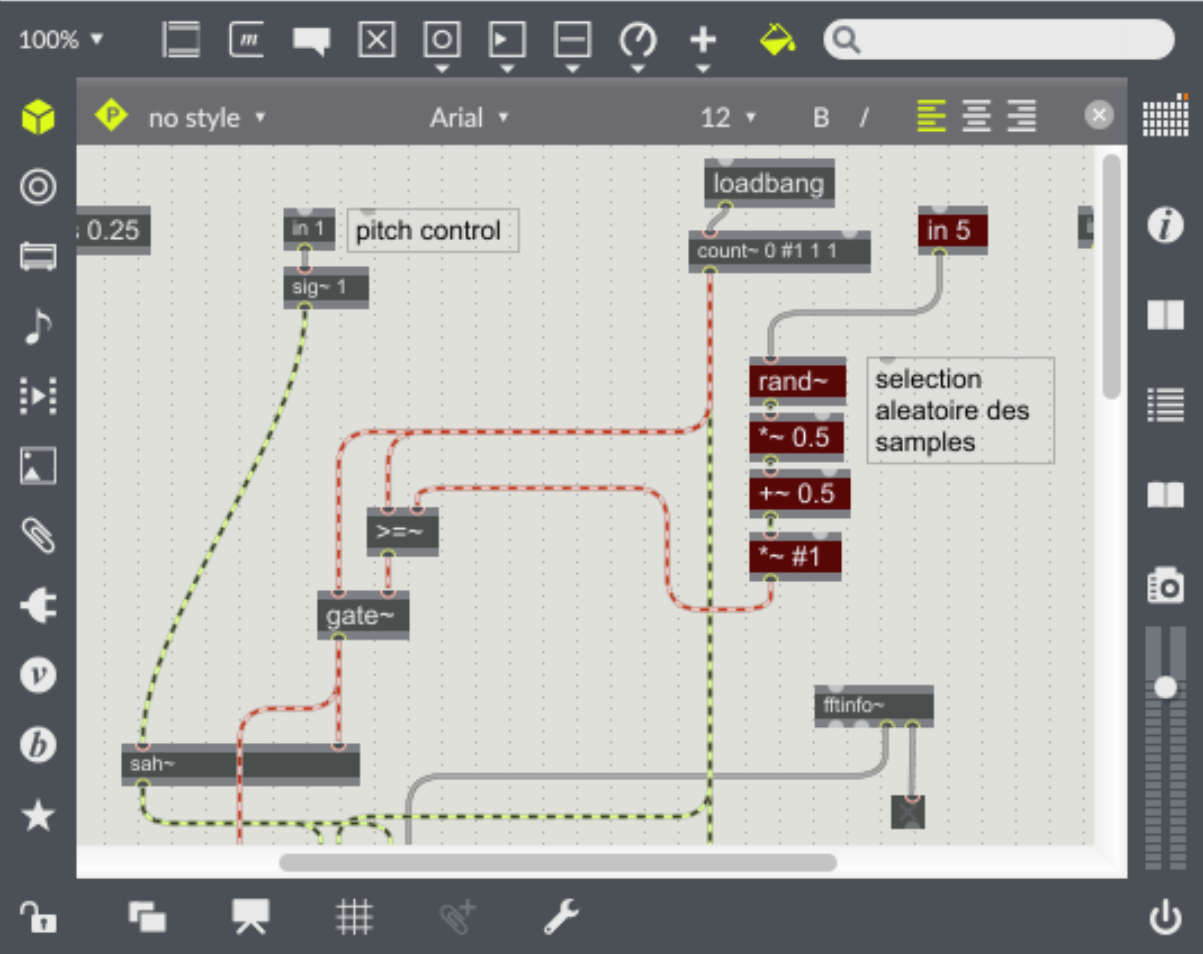
\includegraphics[width=0.48\textwidth]{Graphs/random_sampling.png}
  \end{center}
  \vspace{-20pt}
  \caption{Filtre aletoire}
  \vspace{-10pt}
\end{wrapfigure}

    Le générateur aléatoire est créé par l'objet $ random \thicksim $ avec un filtre modulant la fréquence de la génération de valeur aléatoire. La valeur transmise au lecteur de l'objet $ play \thicksim $ est modulée par un détenteur d'échantillon qui prend en entrée la sortie d'un compteur et la valeur générée de manière aléatoire. Le porte-échantillon est créé manuellement par un objet supérieur à un objet et une porte. De cette manière, nous conservons et publions de manière abstraite des valeurs dans la fenêtre FFT, créant ainsi un système hybride de modulation de la hauteur et de la lecture. La modulation peut être trouvée dans la figure.
    

\section{Morphing visuel}

En avançant sur le morphing visuel, nous avons implémenté le patch suivant avec l’aide du Jitter, pour une interpolation linéaire entre deux dessins.

    \begin{figure}
        \centering
        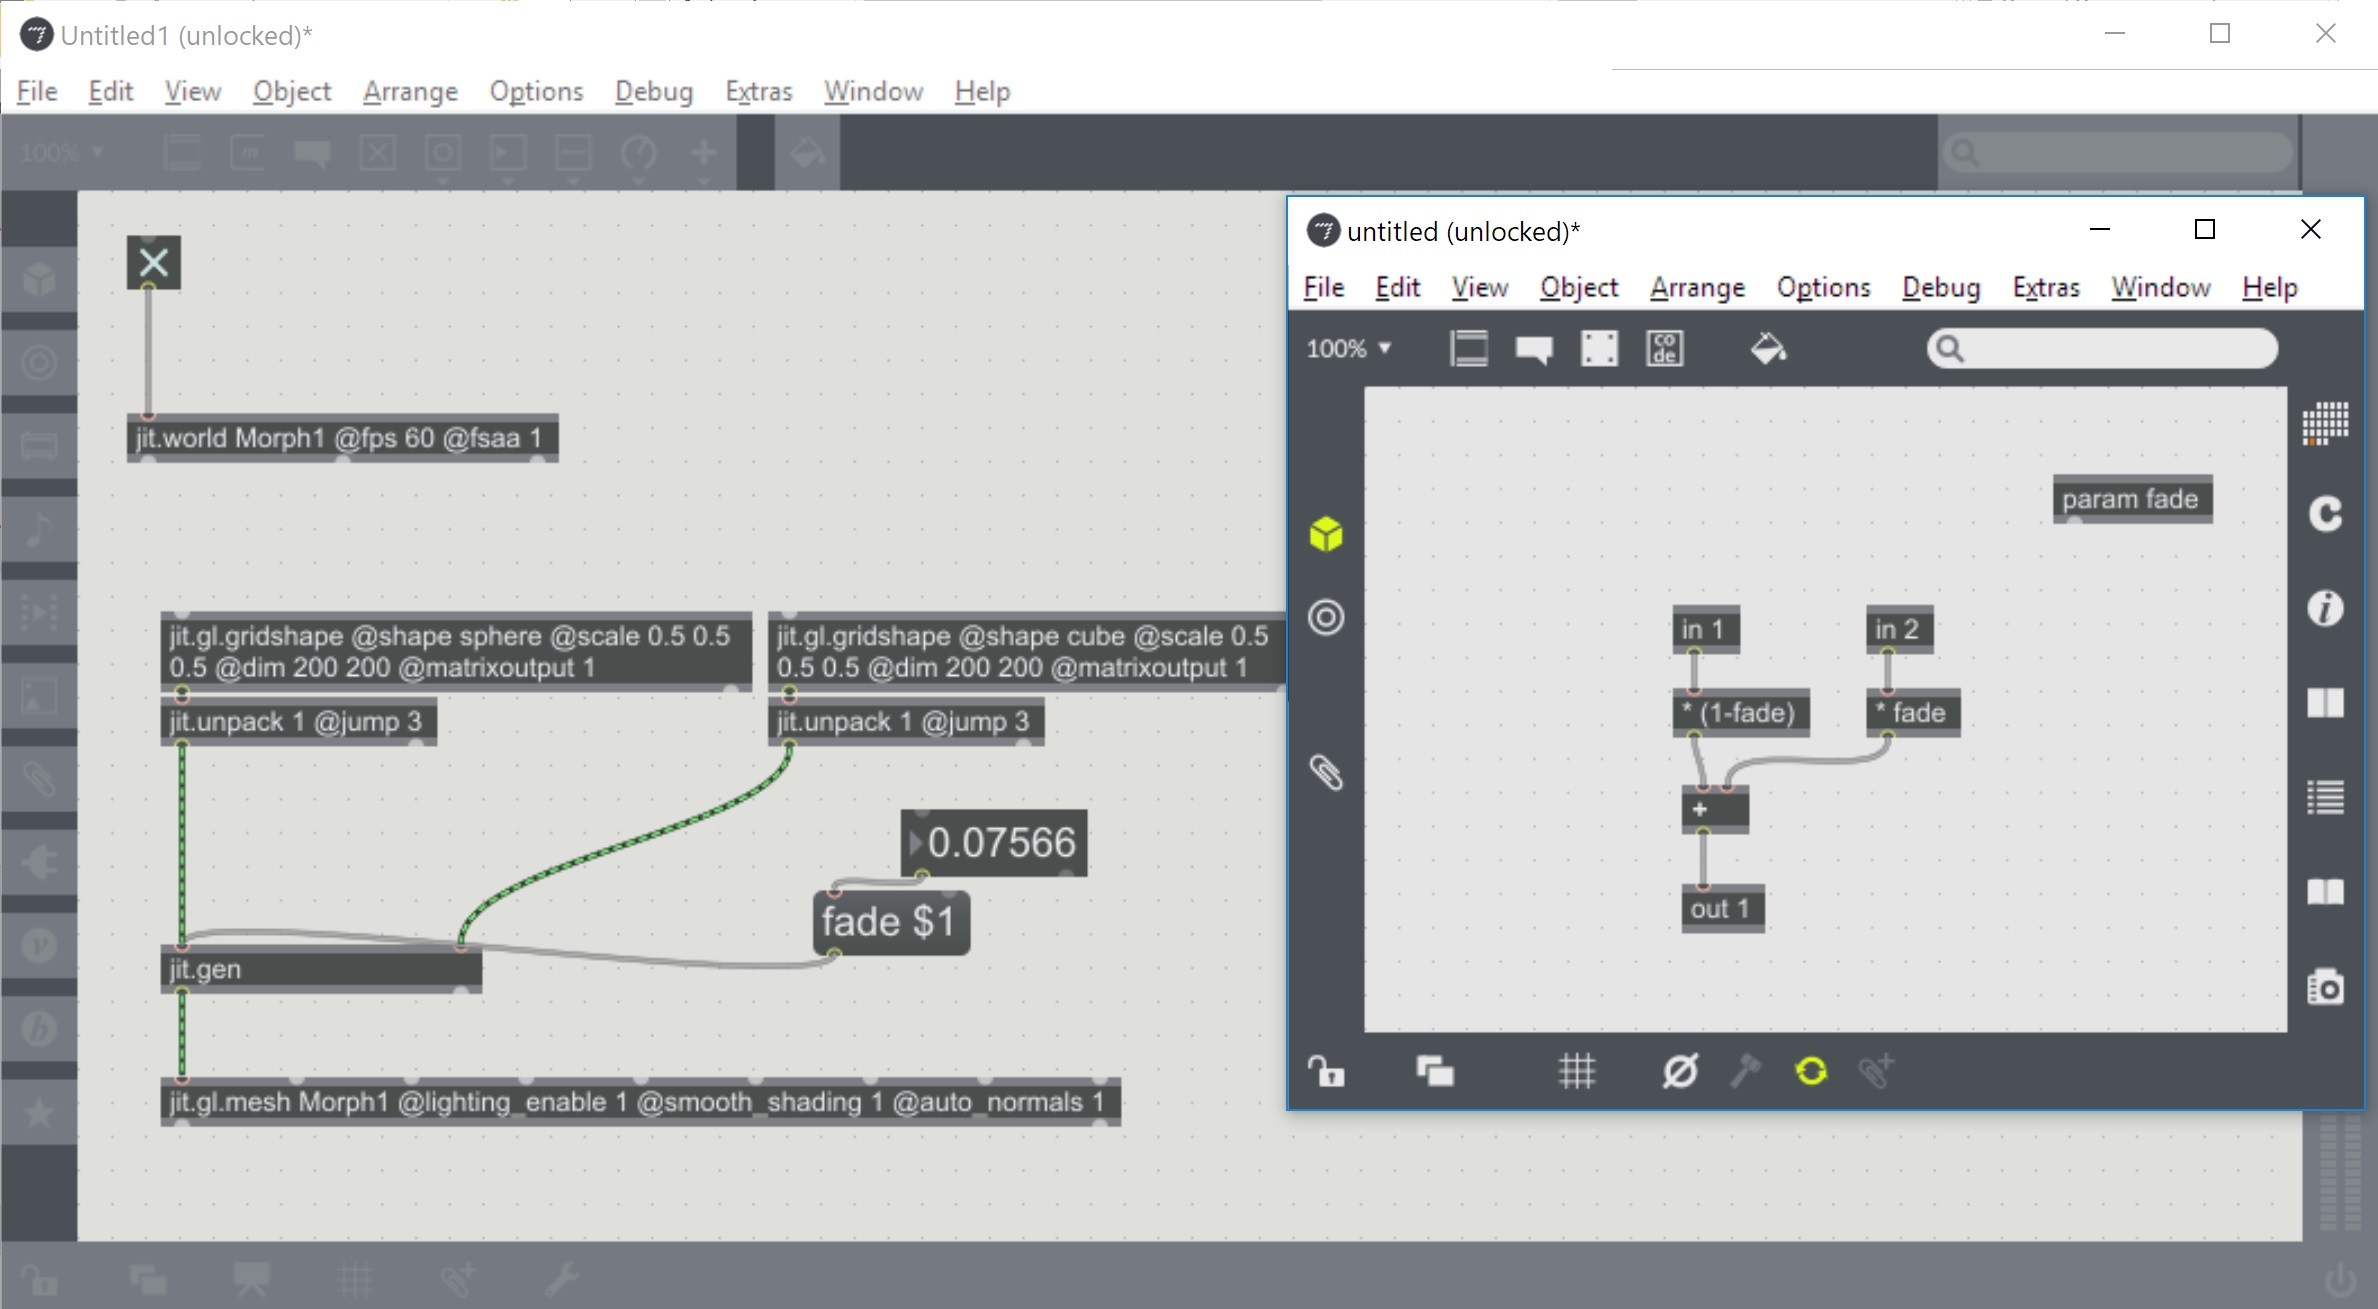
\includegraphics[width = \textwidth ]{Graphs/Morphing_patch.jpg}
        \caption{Visual Morphing}
        \label{VisualMorph}
    \end{figure}


En répétant la formule de base de morphing $M(\alpha) = \alpha\widehat {S_1} + [1 -\alpha]\widehat {S_2} $ une patch sur le morphing en 3D était implémenté avec l'aide de l'objet jit.gen (figure \ref{VisualMorph}).

Donc, fondamentalement, un morphing visuel est facile à faire avec les fonctions 3D primordiaux de Jitter telles que jit.gl.gridshape et jit.gen pour une personnalisation de la procédure de morphing. L'objet jit.gl.mesh est utilisé pour combiner le résultat du morphing alors que l'objet gen est contrôlé par un facteur de fondu.

À l'intérieur de gen, une procédure assez simple se produit. Les données multidimensionnelles provenant des matrices de localisation sont utilisées séparément pour chaque forme et leur amplitude est multipliée par le facteur $\alpha$ comme dans le morphing audio.

Bien entendu, nous pourrions également implémenter le script expondential.js pour une courbe de morphing différente sur le visuel.

Dans le patch suivant nous sommes allés un etape plus loin en separent tout composant d'un modèle tri-dimensionel dans jitter. Nous distinguons les valeurs des matrices, des normals et de la texture. Nous avons ajoutés egalement une interpolation du couleur. Le patch est en disposition en figure \ref{VisualMorph2}.

    \begin{figure}
        \centering
        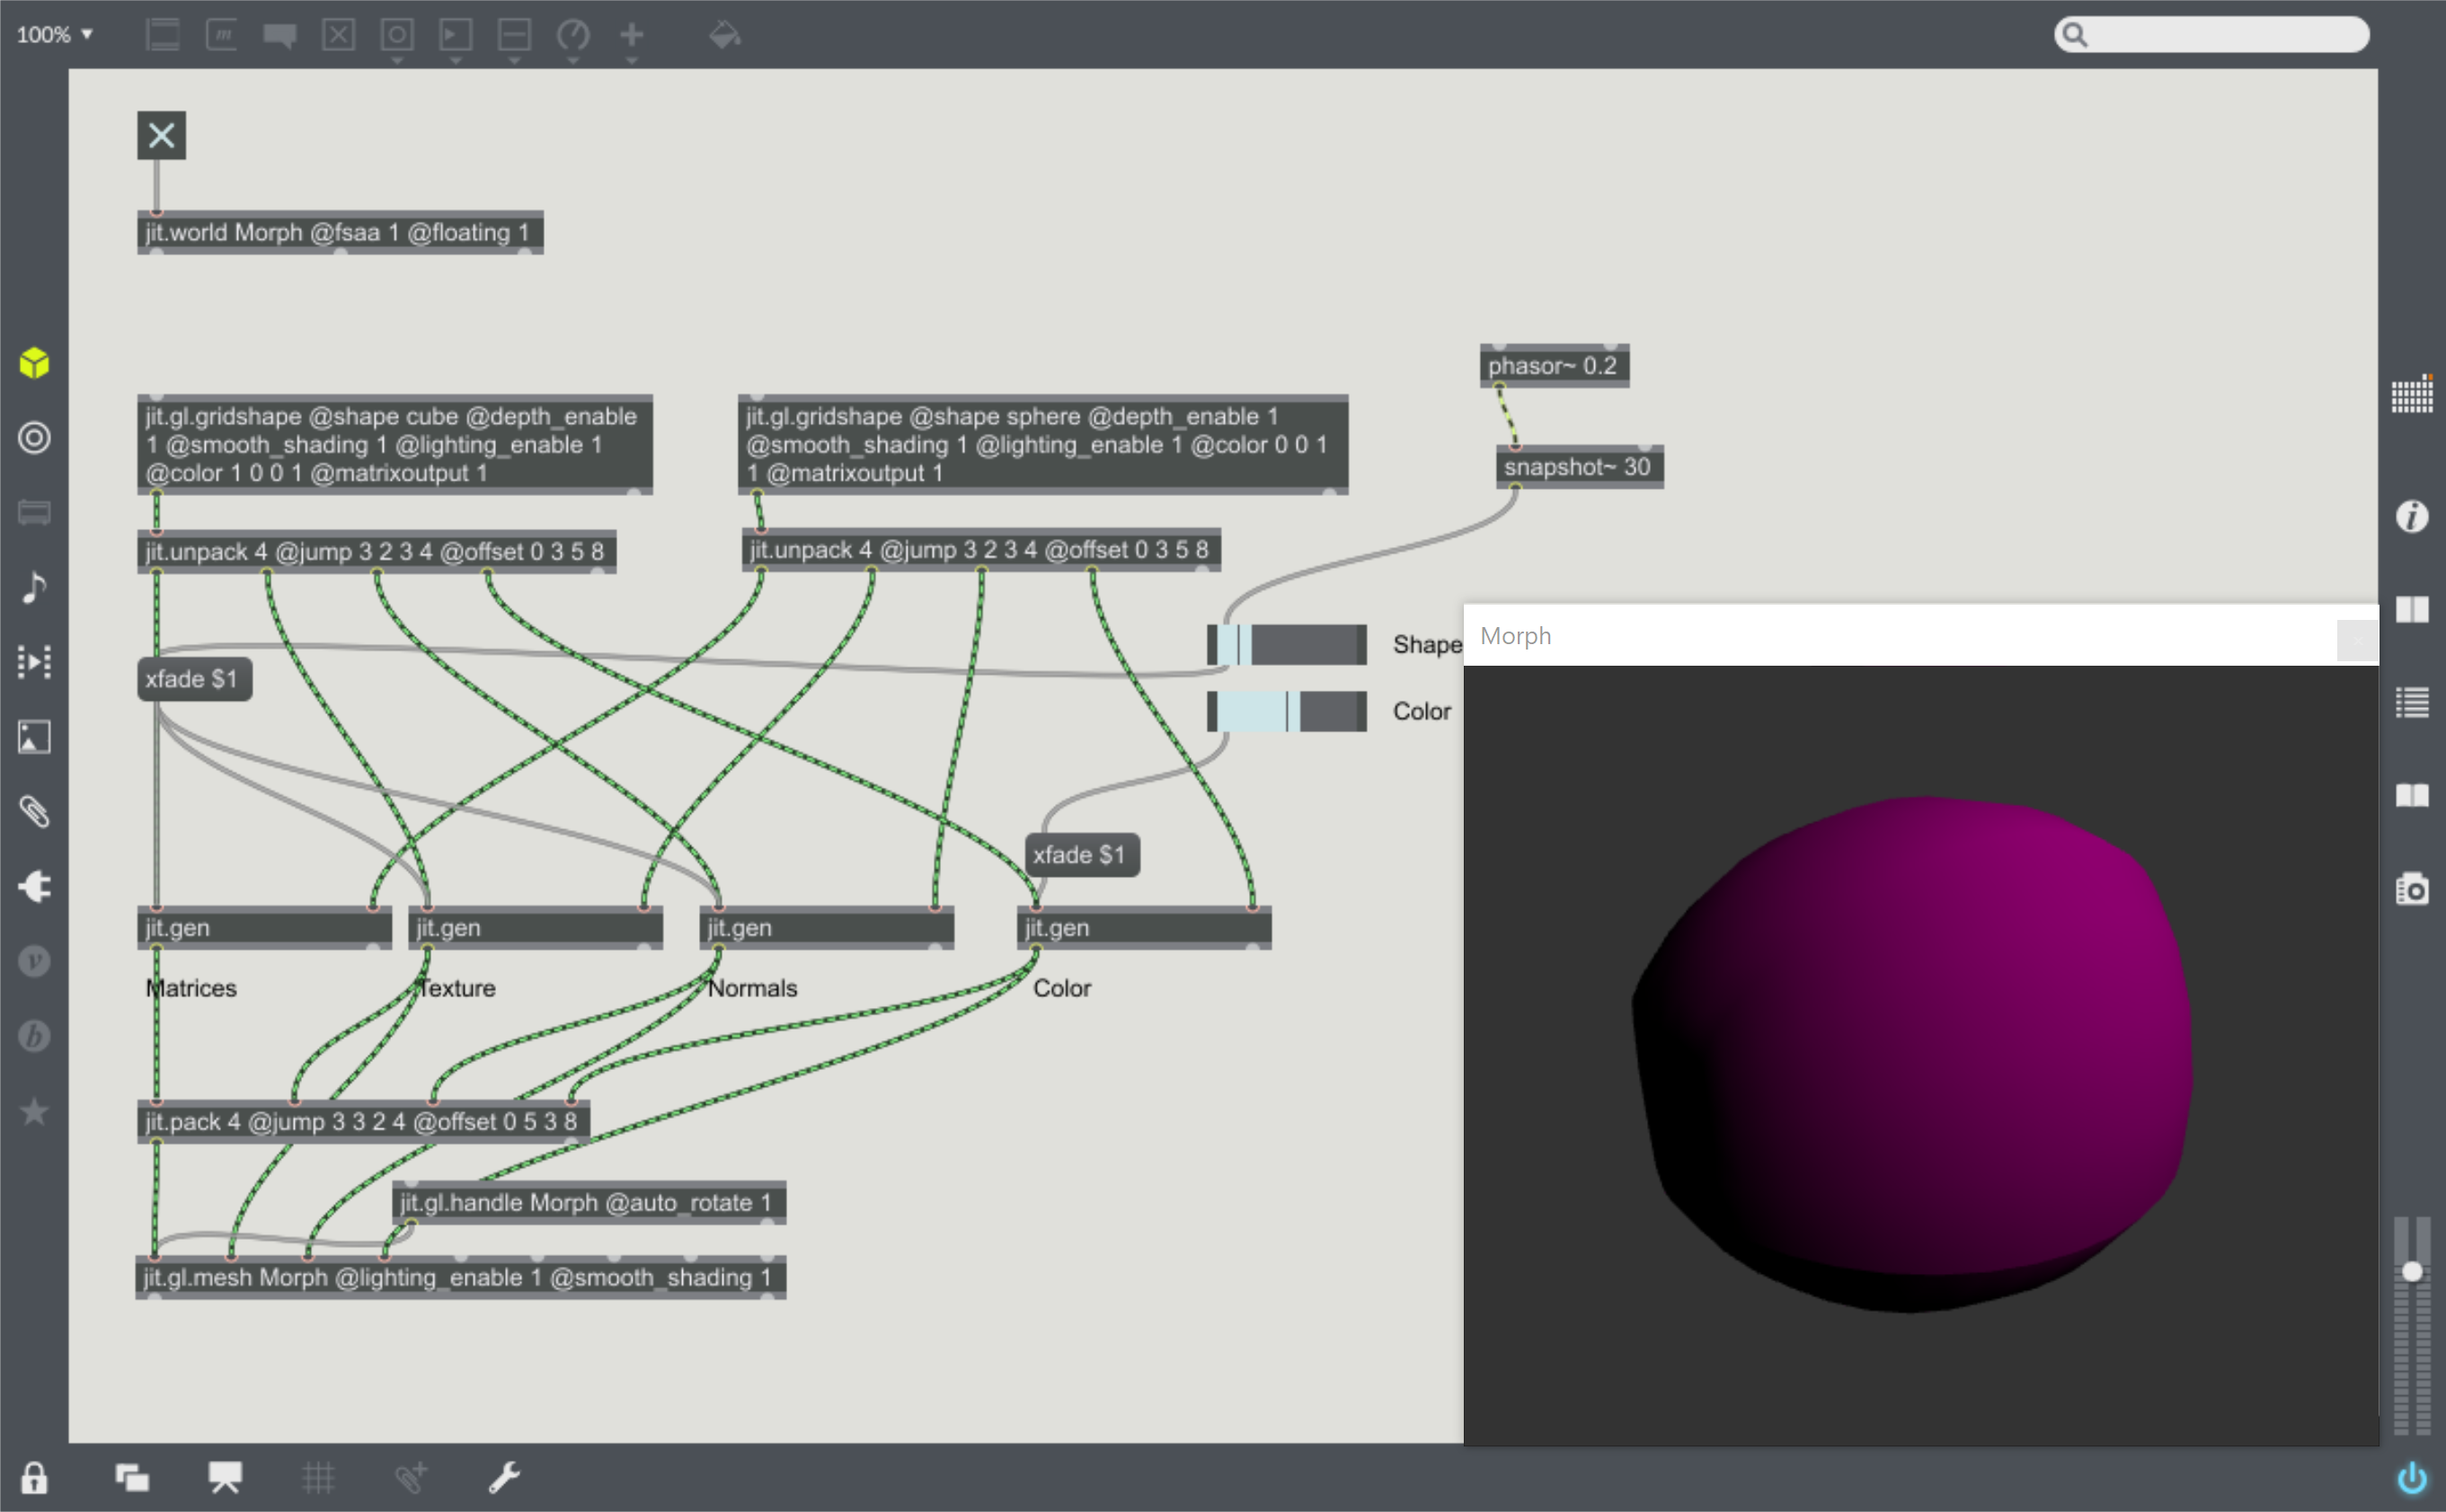
\includegraphics[width = \textwidth ]{Graphs/ShapeMorphing1.png}
        \caption{Visual Morphing $2^{ème}$ version}
        \label{VisualMorph2}
    \end{figure} 

\begin{figure}
\begin{subfigure}{.5\textwidth}
  \centering
  \caption{Interpolation de la forme : $0.0$ \\ Interpolation couleur : $0.0$}
  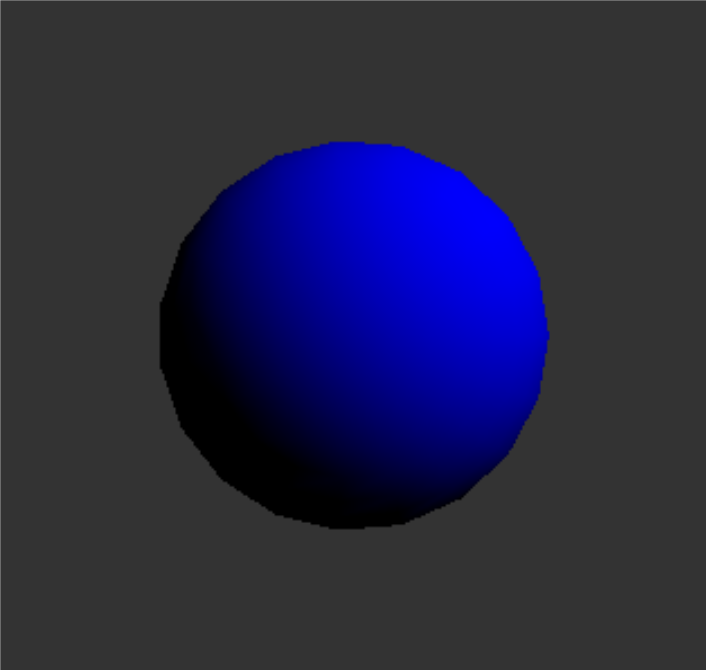
\includegraphics[width=1\linewidth]{Graphs/morph1.png}  
  \label{fig:sub-first}
\end{subfigure}
\begin{subfigure}{.5\textwidth}
  \centering
  \caption{Interpolation de la forme : $0.4$ \\ Interpolation couleur : $0.8$}
  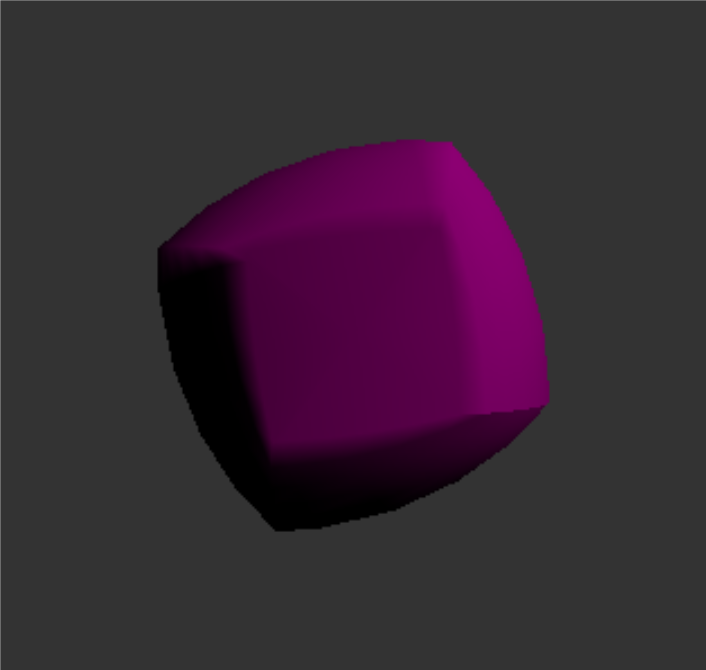
\includegraphics[width=1\linewidth]{Graphs/morph2.png}  
  \label{fig:sub-second}
\end{subfigure}

\begin{subfigure}{.5\textwidth}
  \centering
  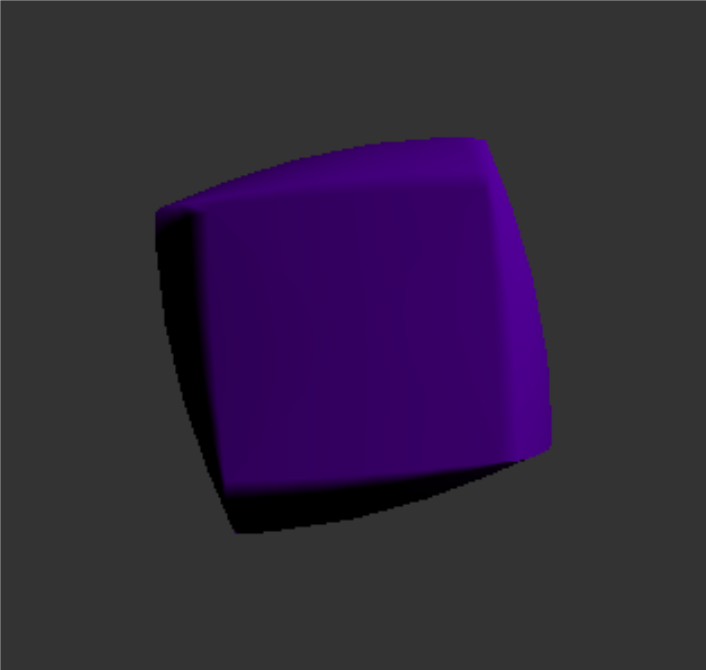
\includegraphics[width=1\linewidth]{Graphs/morph3.png}  
  \caption{Interpolation de la forme : $0.8$ \\ Interpolation couleur : $0.4$}
  \label{fig:sub-third}
\end{subfigure}
\begin{subfigure}{.5\textwidth}
  \centering
  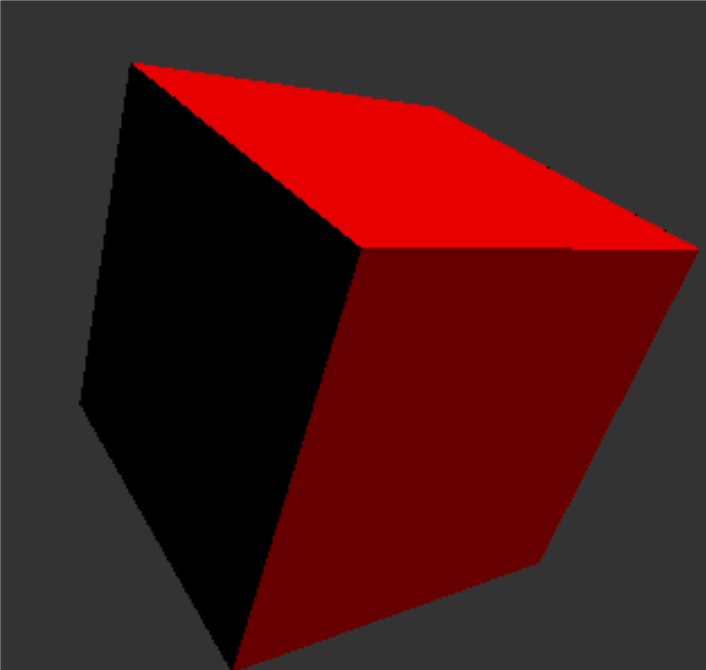
\includegraphics[width=1\linewidth]{Graphs/morph4.png}  
  \caption{Interpolation de la forme : $1.0$ \\ Interpolation couleur : $1.0$}
  \label{fig:sub-fourth}
\end{subfigure}
\caption{Stades du morphing visuel}
\label{fig:fig}
\end{figure}

\subsection{Visualization du spectre}
    
    Dans ce patch, beaucoup de travail sur la gigue a été implémenté avec un vocodeur de phase. Ce code permet de visualiser les informations spectrales d’un son sous la forme d’un paquet de lignes bidimensionnelles imitant les harmoniques trouvées lors d’une analyse de Fourier.

    Ce patch utilisé à l'unisson avec un vocodeur de phase pour le morphing ou même le simple décalage de pitch permet de visualiser l'évolution du spectre dans un environnement de rendu en temps réel. Dans ce code, nous utilisons une bibliothèque de gigue supplémentaire pour produire plusieurs objets de gigue rendus dans un espace tridimensionnel virtuel. L'objectif de cette thèse n'étant pas orienté image, nous ne dévoilerons pas beaucoup d'informations sur le traitement.

    Nous allons attribuer ici brièvement les objets les plus emblématiques de la gigue utilisés dans ce patch. L'objet \textit{jit.world} crée une nouvelle fenêtre et un espace de rendu virtuel tridimensionnel pouvant également contenir de la physique, des plans, des objets tridimensionnels, contrôler la position de la caméra, la couleur d'arrière-plan, etc. Le \textit{jit.gridshape} rend un objet tridimensionnel dans une fenêtre. La bibliothèque \textit{jit.mo} réplique de manière fluide les copies d’objets de gigue. Et le \textit{jit.catch} prend un signal et le traduit en matrice de gigue pour la visualisation potentielle.

    Pour transformer les informations spectrales en données tridimensionnelles, nous utilisons bien sûr une transformation FFT et un tampon qui lit les composantes polaires de la FFT (magnitude et phase) avec un objet $ peek \thicksim $ les envoie dans un tampon. Un objet $ lookup \thicksim $ récupère le contenu du tampon et les entre dans l'objet \textit{jit.catch}.

    Nous pouvons régler la dimension de \textit{jit.mo} pour générer plus d'harmoniques. Le son de sortie du vocodeur est envoyé à ce patch de visualisation harmonique pour saisir le résultat dans un espace 3D.


    \begin{figure}
        \centering
        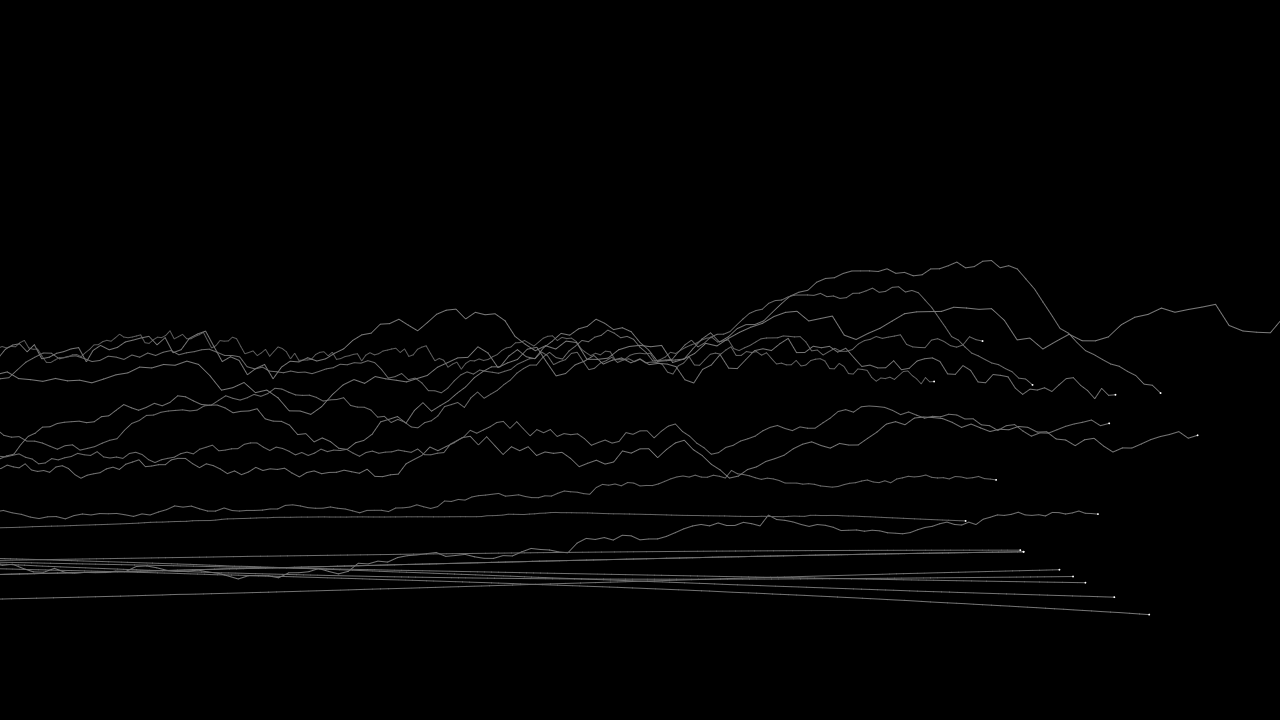
\includegraphics[width = \textwidth ]{Graphs/SpectralWindow.png}
        \caption{Harmoniques dans l'espace}
        \label{SpectralWindow}
    \end{figure} 

    \begin{figure}
        \centering
        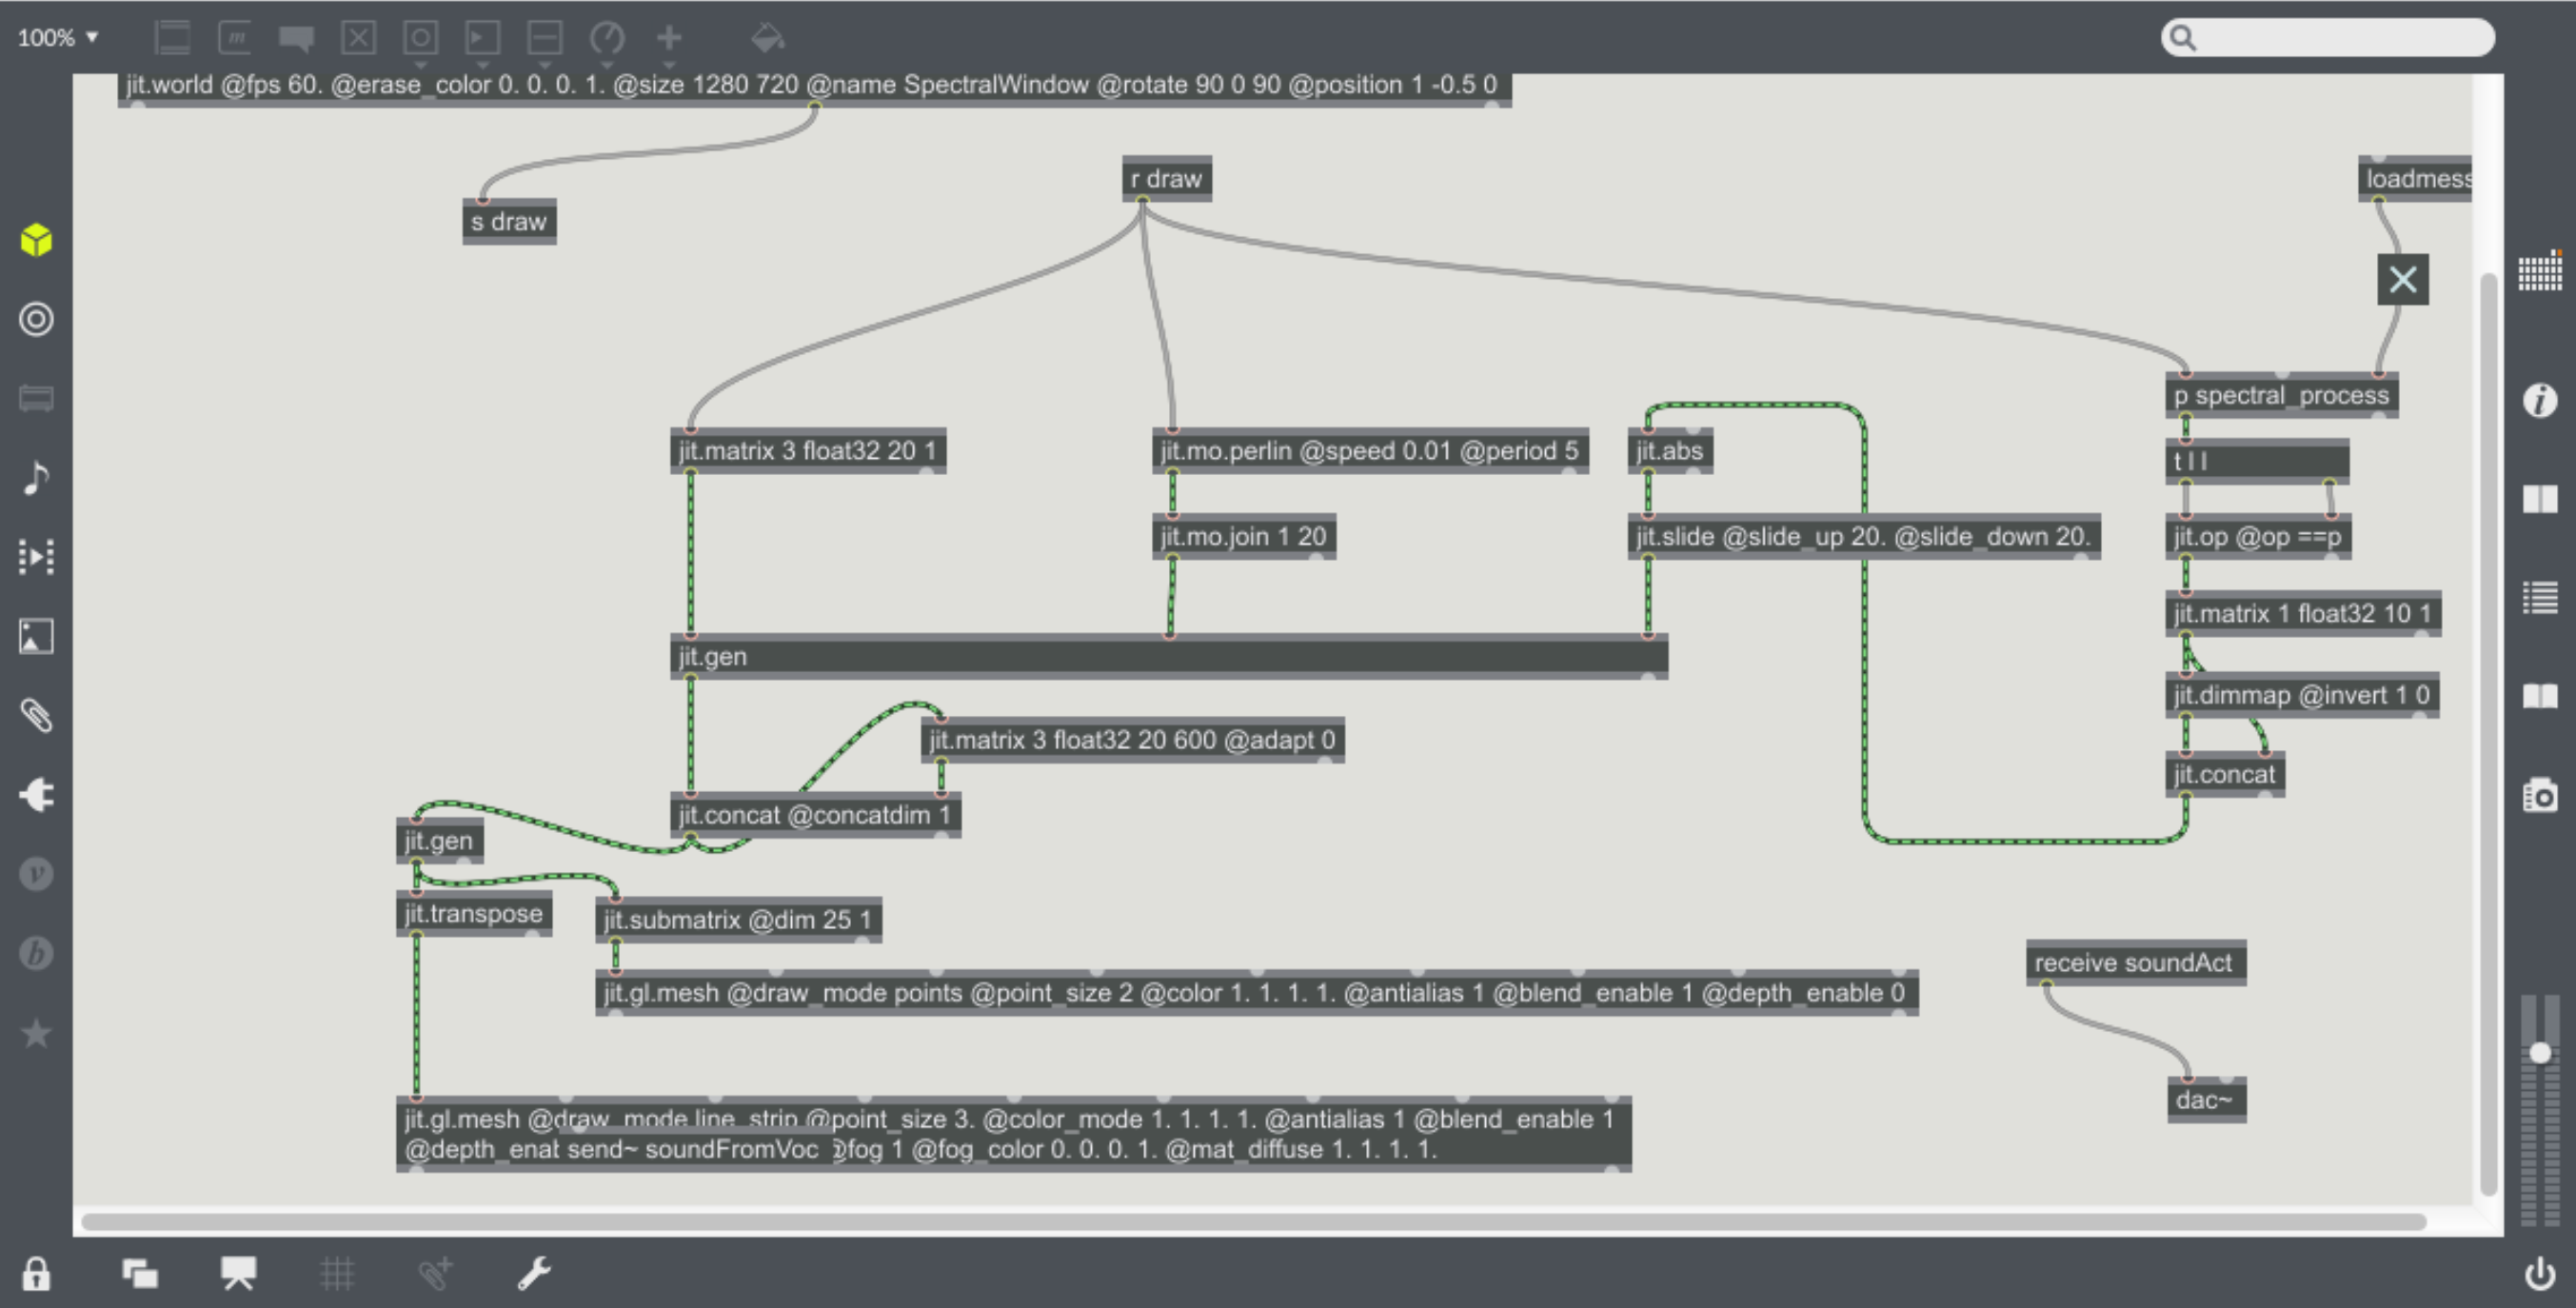
\includegraphics[width = \textwidth ]{Graphs/SpectralDraw.png}
        \caption{Le patch qui control les objets jitter}
        \label{SpectralDraw}
    \end{figure} 


\chapter{Conclusion}
\label{ch:conclusions}

\section{Résumé de la recherche}

%Resumer tout qui était fait.
Dans ce mémoire, nous avons parcouru des notions mathématiques de l'analyse spectrale en se focalisant sur le vocodeur de phase. Nous avons cité toute information nécessaire pour qu'un amateur se plonge dans le domaine du processus spectral du signal. De plus, nous avons détaillé le processus pour créer un vocodeur de phase sur MaxMSP permettant une connaissance plus profonde parmi l'application. En outre, nous avons proposé plusieurs modifications du code dans un contexte artistique et nous avons composé une pièce acousmatique en utilisant ces modifications.

En d'autres termes, cette recherche sert à des fins documentaires ainsi qu'épistémologique. Notre but est d'informer les musiciens et les compositeurs des notions complexes. Ce travail me sera aussi enrichissant, car il m'a permis d'approfondir mes connaissances dans ce domaine. Le spectre est une terminologie difficile à comprendre pour les musiciens et un point de vue plus musical va faciliter sa compréhension. En approfondissant sur le terrain du morphing, on découvre de nouvelles manières pour manipuler cet effet et on applique notre critique. Cette problématique, constitue le but final de la recherche.

\section{Applications}

Dans le second chapitre, nous avons parcouru plusieurs applications du vocodeur de phase mais les capacités de cet outil sont quasiment infinies. Pour donner une idée de ces capacités, le vocodeur de phase peut être utilisé pour analyser la voix et la transformer en texte. Les sélections et les fréquences peuvent être déduites de certaines voyelles et consonnes, ce qui permet de prédire les lettres exactes utilisées et de produire la forme écrite du son\footnote{Axel Roebel, \textit{Shape-invariant speech transformation with the phase vocoder}, 2010.\nocite{roebel2010shape}}.

Le vocodeur de phase qui est appliqué exclusivement sur la voix humaine peut être également modifié pour transformer un certain type de voix. Par exemple une voix d'homme peut être transformée en une voix féminine ou bien tout autre type de voix humaine. Cette opération est construite sur une base des profils spectraux de différents types des voix qui permette d'interpoler entre ces profils spectrales comme un morphing sous paramètres \footnote{Axel Roebel, \textit{A new approach to transient processing in the phase vocoder}, 2003. \nocite{roebel:hal-01161124}}

Une amélioration du vocodeur de phase consiste à appliquer des ondelettes. En lieu d'appliquer la transformation simple de Fourier, on peut remplacer l'exponentiel complexe de Fourier par une fonction d'ondelette. Cette fonction est équivalente de l'application de plusieurs transformées de Fourier à différentes tailles de fenêtres permettant de capter simultanément plus de détail fréquentiel et ponctuel (attaque)\footnote{{Beltr{\'a}n, Jos{\'e} R and Beltr{\'a}n, Fernando}, \textit{Additive synthesis based on the continuous wavelet transform}, 2003.\nocite{beltran2003additive}}. 

Les outils spectraux et spécialement ceux d'analyse-synthèse sont fréquemment utilisés par les compositeurs parmi les logiciels DAW tels que Ableton Live, Cubase, Reaper, etc. Une des  bibliothèques fréquemment utilisée est TRAX fait par \textit{IRCAM Tools} \footnote{\href{https://www.flux.audio/project/ircam-trax-v3/}{https://www.flux.audio/project/ircam-trax-v3/}}.

\section{Discussion}

Le vocodeur de phase est aujourd'hui plus qu'un simple outil d'analyse spectrale. Des méthodes ont été développées pour la prévision de manière stochastique sur une resynthèse optimale des ondes sonores.

Ces méthodes considèrent des formules probabilistes pour reconstruire des signaux afin d’obtenir une meilleure technique de prédiction de la fréquence. Pour plus d'informations à ce sujet, le livre de Roads and al. \footnote{Curtis Roads, Stephen Travis Pope, Aldo Piccialli, Giovanni De Poli, \textit{Musical Signal Processing}, 1997 \nocite{Roads97}} était plutôt éclairant.

\section{Recherche pour l'avenir}

On peut étendre cette recherche sur les processus spectraux en utilisant les principes tels que Deep Learning. Spécifiquement, j'envisage une approche sur le Morphing spectrale en temps réel avec de l'apprentissage pour automatiser la paramétrisation du vocodeur de phase correspondant \footnote{Jesse Engel. Making a neural synthesizer instrument, 2008.}. 

Je suis particulièrement intéressé par le fait qu’un vocoder de phase puisse détecter les fréquences dominantes d'un son. Ce fait pourrait essentiellement servir afin de développer une méthode intelligente pour préciser les différentes notes contenue dans un son polyphonique \footnote{Polyphonie : Assemblage de voix ou d'instruments, sans préjuger de leur nature}. L'extraction des fréquences dominantes de chaque voix en forme de notes pourrait assister à l'analyse automatique de la musique à partir des fichiers sonores et, par suite, transformer le son à une forme symbolique. Dans une prochaine recherche, je souhaiterais aborder le domaine de l'analyse Topologique de la musique. C’est une interprétation de la musique symbolique comme des structures topologiques bidimensionnelles, c'est-à-dire des graphes orientés. À partir de ces graphes on pourra extraire des informations du style musical ou de la structure harmonique d”une pièce musicale. La théorie de graphes contient plusieurs méthodes spectrales telles que la transformation Fourier des graphes et toute une infrastructure mathématique basée sur les concepts investigués dans ce mémoire.

Une  des pistes alternatives, également intéressante à étudier pour ma part,, serait l’utilisation des VAE (Variational Autoencoders) pour identifier la distribution de probabilité d’un ensemble de pièces musicales. Les VAE sont des auto-encodeurs qui paramètrent la distribution de probabilité des variables latentes à l'aide d'un réseau neuronal et maximisent la probabilité que la distribution de données soit soumise à des contraintes de la distribution de variables latentes. Des expériences numériques montrent qu’il est capable d’identifier cette distribution de données dans la mesure où l’échantillonnage à partir de la distribution de variables latentes génère des points de données réalistes. J'aspire à utiliser cette représentation pour produire une nouvelle musique en combinant d'autres pièces musicales dans l'intégration VAE.

Je crois que le processus d'analyse musicale sur l'harmonie et la mélodie, associé à un apprentissage non supervisé, permet de passer à de meilleurs modèles de prédiction musicale, de variation et de créativité. Pour atteindre cet objectif, je visualise la première formalisation de modélisation algébrique sur des données verticales (accords) et linéaires (mélodies) telles que les approches de la théorie de la musique transformationnelle. Avant de construire une base de données de styles et d’appliquer un algorithme de prédiction, j’estime que, grâce à VAE, cela peut être avancé et produire des résultats révolutionnaires.
Jusqu'à présent, VAE présentait une application limitée aux données séquentielles et les modèles existants de VAE récurrents rencontraient des difficultés pour modéliser des séquences avec une structure à long terme. Pour résoudre ce problème, je propose l’utilisation d’un décodeur hiérarchique, qui génère d’abord des intégrations pour les sous-séquences de l’entrée, puis utilise ces intégrations pour générer chaque sous-séquence de manière indépendante. Il est également possible de modéliser de la musique polyphonique multipiste en tant que vecteurs dans un espace latent via le conditionnement d'accords. En effet celui-ci permet une compréhension plus profonde de la mélodie tout en maintenant une harmonie fixe, et permet en outre de modifier les accords tout en maintenant le style musical. Cette approche a été présentée pour la première fois dans le projet Magenta de Google AI et présente, à mon avis, un potentiel important et pourrait progresser dans la génération simultanée d'accords et de mélodies.

\appendix
\chapter{Appendix}

\label{ch:Appendix}

	\section{FFT Cooley - Tukey algorithm}
	\label{Cooley-Tukey_Code} 

	\begin{lstlisting}[language=C, caption= Cooley-Tukey with Butterfly Diagrams ]
		using FFTW
		#simple DFT function
		function DFT(x)s
		    N = length(x)
		    # We want two vectors here for real space (n) and frequency space (k)
		    n = 0:N-1
		    k = n'
		    transform_matrix = exp.(-2im*pi*n*k/N)
		    return transform_matrix*x
		end
		# Implementing the Cooley-Tukey Algorithm
		function cooley_tukey(x)
		    N = length(x)
		    if (N > 2)
		        x_odd = cooley_tukey(x[1:2:N])
		        x_even = cooley_tukey(x[2:2:N])
		    else
		        x_odd = x[1]
		        x_even = x[2]
		    end
		    n = 0:N-1
		    half = div(N,2)
		    factor = exp.(-2im*pi*n/N)
		    return vcat(x_odd .+ x_even .* factor[1:half],
		                x_odd .- x_even .* factor[1:half])
		end
		function bitreverse(a::Array)
		    # First, we need to find the necessary number of bits
		    digits = convert(Int,ceil(log2(length(a))))

		    indices = [i for i = 0:length(a)-1]

		    bit_indices = []
		    for i = 1:length(indices)
		        push!(bit_indices, bitstring(indices[i]))
		    end
		    # Now stripping the unnecessary numbers
		    for i = 1:length(bit_indices)
		        bit_indices[i] = bit_indices[i][end-digits:end]
		    end
		    # Flipping the bits
		    for i =1:length(bit_indices)
		        bit_indices[i] = reverse(bit_indices[i])
		    end
		    # Replacing indices
		    for i = 1:length(indices)
		        indices[i] = 0
		        for j = 1:digits
		            indices[i] += 2^(j-1) * parse(Int, string(bit_indices[i][end-j]))
		        end
		       indices[i] += 1
		    end
		    b = [float(i) for i = 1:length(a)]
		    for i = 1:length(indices)
		        b[i] = a[indices[i]]
		    end
		    return b
		end
		function iterative_cooley_tukey(x)
		    N = length(x)
		    logN = convert(Int,ceil(log2(length(x))))
		    bnum = div(N,2)
		    stride = 0;
		    x = bitreverse(x)
		    z = [Complex(x[i]) for i = 1:length(x)]
		    for i = 1:logN
		       stride = div(N, bnum)
		       for j = 0:bnum-1
		           start_index = j*stride + 1
		           y = butterfly(z[start_index:start_index + stride - 1])
		           for k = 1:length(y)
		               z[start_index+k-1] = y[k]
		           end
		       end
		       bnum = div(bnum,2)
		    end
		    return z
		end
		function butterfly(x)
		    N = length(x)
		    half = div(N,2)
		    n = [i for i = 0:N-1]
		    half = div(N,2)
		    factor = exp.(-2im*pi*n/N)

		    y = [0 + 0.0im for i = 1:length(x)]

		    for i = 1:half
		        y[i] = x[i] + x[half+i]*factor[i]
		        y[half+i] = x[i] - x[half+i]*factor[i]
		    end
		    return y
		end
		function approx(x, y)
		    val = true
		    for i = 1:length(x)
		        if (abs(x[i]) - abs(y[i]) > 1e-5)
		            val = false
		        end
		    end
		    println(val)
		end
		function main()
		    x = rand(128)
		    y = cooley_tukey(x)
		    z = iterative_cooley_tukey(x)
		    w = fft(x)
		    approx(y, w)
		    approx(z, w)
		end
		main()
	\end{lstlisting}\footnote{Le code est recuperé sur le lien \href{https://www.algorithm-archive.org/contents/cooley_tukey/cooley_tukey.html}{www.algorithm-archive.org} distribué sous la licence \textit{MIT}}.


	\section{Espace $L^p$ et STFT}

	La STFT est une version locale de la transformée de Fourier. Normalement, pour effectuer la transformation de Fourier, on part d'une fonction $f(x)$ qui appartient à l'espace Lebesque $L^{2} (\mathbb{R}^k)$ soit à $L^{1} (\mathbb{R}^k)$ et on obtient une fonction $\hat{f}(\omega)$ qui appartient respectivement à $L^{2} (\mathbb{R}^k)$ ou à $C_{0}(\mathbb{R}^{k})$\footnote{L'espace des fonctions continues qui tendent vers $0$ à l'infini}.

	Soit $f:\mathbb{R}^k \rightarrow \mathbb{C}, \; f \| L^1(\mathbb{R}^k)$.

	On définit la transformée de Fourier de $f$ et on la note $\mathcal{F}f$ ou $\mathcal{F}[f]$ ou encore $\hat{f}$ par
	$$
	\begin{matrix}
	\hat{f} & : & \mathbb{R}^k & \rightarrow & \mathbb{C}			 &    & \\
			&   & \omega & \mapsto     & \hat{f}(\omega) & := & \int_{\mathbb{R}^k}f(x)e^{-2 \pi i x \cdot \omega} dx
	\end{matrix}
	$$

	En effet, la transformée de Fourier peut être définie pour des fonctions de $L^2(\mathbb{R}^k)$ et par le théorème de Plancherel :

	Si $f \in L^1(\mathbb{R}^k) \cap L^2(\mathbb{R}^k)$ alors 
	$$\| {f}_{2} \| = \|\hat{f}\|_{2}$$
	et donc l'opérateur $\mathcal{F}$ peut être étendu à $L^2(\mathbb{R}^k)$. De plus, on a ce qu'on appelle l'identité de Parseval
	$$ \langle f, g \rangle = \langle \hat{f}, \hat{g} \rangle \, , \quad \forall f,g \in L^2(\mathbb{R}^k) $$

	En somme, la transformée de Fourier est un isomorphisme isométrique de $L^2(\mathbb{R}^k)$ en $L^2(\mathbb{R}^k)$, ce qui de manière symbolique est traduit par
	$$
	\begin{matrix}
	\mathcal{F} : & L^2(\mathbb{R}^k) & \rightarrow & L^2(\mathbb{R}^k) \\
	& f & \mapsto & \hat{f}
	\end{matrix}
	$$
	et
	$$ \mathcal{F} \circ \mathcal{F}^{-1} = \mathcal{F}^{-1} \circ \mathcal{F} = Id $$

	Pour effectuer la STFT on doit d'abord fixer une fonction qui nous servira de fenêtre. Dans une approche plus practique, on utilisera généralement des fonctions avec une formte décroissance à l'infini (par exemple une fonction gaussienne). De cette manière on pourra appliquer la STFT à des fonctions qui n'ont peut-être pas de transformée de Fourier ordinaire. On laissera les détails de quelles fonctions sont celles qui admettent une STFT (en fonction de la fenêtre fixée) pour plus tard et on se contentera d'abord de voir que si $g\in L^{p}(\mathbb{R}^{k})$ alors toute $f\in L^{p'} (\mathbb{R}^k)$ admet une STFT.

	Pour appliquer la STFT à une fonction il faut être sur que le résultat sera bien défini; cela nous rapporte au problème de choisir un domaine de définition pour la STFT.
	Dans la définition de la STFT on a choisit comme domaines pour $f$ et pour $g$ respectivement $L^{p'} (\mathbb{R}^k) $ et $L^p (\mathbb{R}^k)$. Ce choix a été fait pour la première approche mais le fait est que la STFT peut être étendue à bien d'autres espaces, notament des espaces de distributions.

	Dans cette section on va proposer quelques uns (ceux qui sont présentés en \cite{Grochenig}); loin d'être une exposition exhaustive, on ne présentera que les espaces les plus importants dans le cadre de l'analyse de Fourier. L'étude détaillé du cas des espaces de modulation sera laissé pour quand ceux-là seront présentés.

	On rappelle qu'on utilise $\mathscr{D} (\mathbb{R}^k)$ pour noter l'espace des distributions ordinaires et $\mathscr{T} (\mathbb{R}^k)$ pour noter l'espace des distributions tempérées.

	Soit $E$ indifféremment $C^{\infty}_{c} (\mathbb{R}^{k})$ (l'espaces des fonctions lisses à support compact) ou $\mathscr{T} (\mathbb{R}^k)$ et soit $\langle \cdot , \cdot \rangle$ son crochet de dualité.

	$$
	\begin{matrix}
	V_{g}\sigma : & \mathbb{R}^d \times \mathbb{R}^k & \rightarrow & \mathbb{C} \\
	& (t,\omega) & \mapsto & V_{g}\sigma (t, \omega) &=& \sigma(M_{\omega}T_{t}g) := \langle \sigma, M_{\omega}T_{t}g \rangle 
	\end{matrix}
	$$
	et on obtient une extension de la STFT.

	Cette définition n'a pas besoin de justification; en effet, l'évaluation de la distribution dans un élément de son domaine est bien évidemment définie. On pourrait se demander si les opérateurs $M_{\omega}$ et $T_{t}$ laissent invariant les espaces $C^{\infty}_{c}(\mathbb{R}^{d})$ et $\mathscr{T} (\mathbb{R}^k)$. De plus, la justification de que ce soit une extension est faite par l'interpretation de toute fonction de $E$ comme élément de $E'$ par le crochet de dualité.

	Cela nous dit de plus que si $B$ est un espace de Banach contenu dans $\mathscr{T} (\mathbb{R}^k)$ qui est invariant par des traslations et modulations alors la STFT est bien définie pour $f\in B'$ et $g\in B$.
\lstlistoflistings 

\bibliographystyle{plainnat}
\bibliography{biblio}

% \nocite{*}

\end{document}{}